\chapter{Vectors in Euclidean Space}
\label{chapter:vectors}
%Begin Section 1.1
\section{Introduction}
In single-variable calculus, the functions that one encounters are functions of a variable (usually $x$ or $t$) 
that varies over some subset of the real number line (which we denote by $\mathbb{R}$).  For such a function, say,
$y = f(x)$, the \textbf{graph} of the function $f$ consists of the points $(x, y) = (x, f(x))$.  These points lie in
the \textbf{Euclidean plane}\index{plane!Euclidean}, which, in the \textbf{Cartesian}\index{coordinates} or
\textbf{rectangular}\index{coordinates!rectangular} coordinate system, consists\index{function}
of all ordered pairs of real numbers $(a, b)$.  We use the word ``Euclidean'' to denote a system in which all the
usual rules of Euclidean geometry hold.  We denote the Euclidean plane by $\Real{2}$\index{$\Real{2}$};
the ``2'' represents\index{coordinates!Cartesian}
the number of \emph{dimensions} of the plane.  The Euclidean plane has two perpendicular
\textbf{coordinate axes}: the $x$-axis and the $y$-axis.

In vector (or multivariable) calculus, we will deal with functions of two or three variables (usually $x, y$ or
$x, y, z$, respectively).  
The graph of a function of two variables, say, $z = f(x,y)$, lies in \textbf{Euclidean space}\index{Euclidean space}, which in the Cartesian coordinate system consists of all ordered
triples of real numbers $(a, b, c)$.  Since Euclidean space is 3-dimensional, we denote it by
$\Real{3}$\index{$\Real{3}$}.  The graph of $f$ consists
of the points $(x, y, z) = (x, y, f(x, y))$.  The 3-dimensional coordinate system of Euclidean space can be
represented on a flat surface, such as this page or a blackboard, only by giving the illusion of three
dimensions, in the manner shown in Figure \ref{fig:euc1}.  Euclidean space has three mutually perpendicular
coordinate axes ($x, y$ and $z$), and three mutually perpendicular coordinate planes\index{plane!coordinate}:
the $xy$-plane, $yz$-plane and $xz$-plane (see Figure \ref{fig:euc2}).
\newline
\begin{figure}[h]
\begin{minipage}[t]{7.5cm}
 \begin{center}
  \includegraphics{fig1.1.1.0}
 \end{center}
 \caption[]{}
 \label{fig:euc1}
\end{minipage}
\begin{minipage}[t]{7.5cm}
 \begin{center}
  \includegraphics{fig1.1.2.0}
 \end{center}
 \caption[]{}
 \label{fig:euc2}
\end{minipage}
\end{figure}

The coordinate system shown in Figure \ref{fig:euc1} is known as a
\textbf{right-handed coordinate system}\index{coordinates!right-handed}, because
it is possible, using the right hand, to point the index finger in the positive direction of the $x$-axis,
the middle finger in the positive direction of the $y$-axis, and the thumb in the positive direction of the
$z$-axis, as in Figure \ref{fig:rhs}.

\begin{figure}[h]
 \begin{center}
  %% Creator: Inkscape inkscape 0.48.1, www.inkscape.org
%% PDF/EPS/PS + LaTeX output extension by Johan Engelen, 2010
%% Accompanies image file 'righthand.eps' (pdf, eps, ps)
%%
%% To include the image in your LaTeX document, write
%%   \input{<filename>.pdf_tex}
%%  instead of
%%   \includegraphics{<filename>.pdf}
%% To scale the image, write
%%   \def\svgwidth{<desired width>}
%%   \input{<filename>.pdf_tex}
%%  instead of
%%   \includegraphics[width=<desired width>]{<filename>.pdf}
%%
%% Images with a different path to the parent latex file can
%% be accessed with the `import' package (which may need to be
%% installed) using
%%   \usepackage{import}
%% in the preamble, and then including the image with
%%   \import{<path to file>}{<filename>.pdf_tex}
%% Alternatively, one can specify
%%   \graphicspath{{<path to file>/}}
%% 
%% For more information, please see info/svg-inkscape on CTAN:
%%   http://tug.ctan.org/tex-archive/info/svg-inkscape

\begingroup
  \makeatletter
  \providecommand\color[2][]{%
    \errmessage{(Inkscape) Color is used for the text in Inkscape, but the package 'color.sty' is not loaded}
    \renewcommand\color[2][]{}%
  }
  \providecommand\transparent[1]{%
    \errmessage{(Inkscape) Transparency is used (non-zero) for the text in Inkscape, but the package 'transparent.sty' is not loaded}
    \renewcommand\transparent[1]{}%
  }
  \providecommand\rotatebox[2]{#2}
  \ifx\svgwidth\undefined
    \setlength{\unitlength}{277.909pt}
  \else
    \setlength{\unitlength}{\svgwidth}
  \fi
  \global\let\svgwidth\undefined
  \makeatother
  \begin{picture}(1,0.78089537)%
    \put(0,0){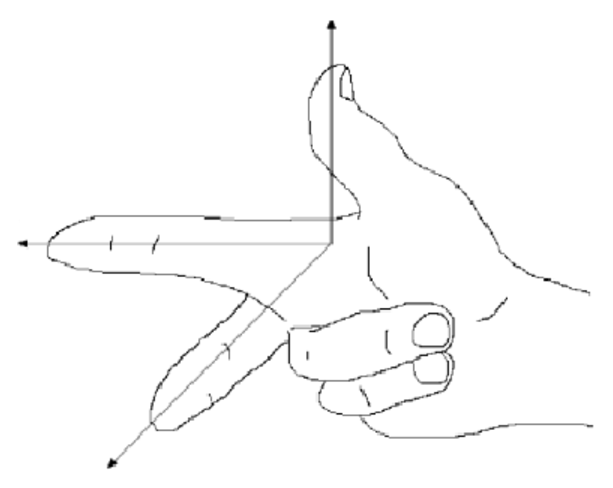
\includegraphics[width=\unitlength]{righthand.eps}}%
    \put(0.00631322,0.42986157){\color[rgb]{0,0,0}\makebox(0,0)[lb]{\smash{$x$}}}%
    \put(0.5863592,0.76090519){\color[rgb]{0,0,0}\makebox(0,0)[lb]{\smash{$z$}}}%
    \put(0.21069667,0.00814079){\color[rgb]{0,0,0}\makebox(0,0)[lb]{\smash{$y$}}}%
    \put(0.535983,0.33342713){\color[rgb]{0,0,0}\makebox(0,0)[lb]{\smash{0}}}%
  \end{picture}%
\endgroup

 \end{center}
 \caption[]{\quad Right-handed coordinate system.}
 \label{fig:rhs}
\end{figure}

An equivalent way of defining a right-handed system is if you can point your thumb upwards in the positive
$z$-axis direction while using the remaining four fingers to rotate the $x$-axis towards the $y$-axis.
Doing the same thing
with the left hand is what defines a \textbf{left-handed coordinate system}\index{coordinates!left-handed}.
Notice that switching the $x$- and $y$-axes
in a right-handed system results in a left-handed system, and that rotating either type of system does not change its ``handedness''.  
Throughout the book we will use a right-handed system.

For functions of three variables, the graphs exist in 4-dimensional space ($\Real{4}$),
which we can not see in our 3-dimensional space, let alone simulate in 2-dimensional space.  
So we can only think of 4-dimensional space abstractly.  For an entertaining discussion of this subject, see the book by \cite{abb}.%
\footnote{One thing you will learn is why a 4-dimensional creature would be able to reach inside an egg and remove the yolk without cracking the shell!}

So far, we have discussed the \emph{position} of an object in 2-dimensional or 3-dimensional space.
But what about something such as the velocity\index{velocity} of the object, or its acceleration\index{acceleration}?
Or the gravitational force acting on the object? These phenomena all seem to involve motion and \emph{direction} in some
way.  This is where the idea of a \emph{vector} comes in.

You have already dealt with velocity and acceleration in single-variable calculus.  For example, for motion along a
straight line, if $y = f(t)$ gives the displacement of an object after time $t$, then $dy/dt = f\,'(t)$ is the velocity
of the object at time $t$.  
The derivative\index{derivative}
$f\,'(t)$ is just a number, which is positive if the object is moving in an
agreed-upon ``positive'' direction, and negative if it moves in the opposite of that direction. So you can think of
that number, which was called the velocity of the object, as having two components: a \emph{magnitude}, indicated by
a nonnegative number, preceded by a \emph{direction}, indicated by a plus or minus symbol (representing motion in the
positive direction or the negative direction, respectively); that is, $f\,'(t) = \pm a$ for some number $a \ge 0$.  
Then
$a$ is the magnitude of the velocity (normally called the \emph{speed} of the object), and the $\pm$ represents the
direction of the velocity (though the $+$ is usually omitted for the positive direction).

For motion along a straight line 
(which is a 1-dimensional space) 
the velocities are also contained in that 1-dimensional space, since they are just numbers.  
For general motion along a curve in 2- or 3-dimensional space,
however, velocity will need to be represented by a multidimensional object which should have both a magnitude and a
direction.  
A geometric object which has those features is an arrow, which in elementary geometry is called a
``directed line segment''.  This is the motivation for how we will define a vector\index{vector}.

\statedefn{defn:vec}{
 {A (nonzero) \textbf{vector} is a directed line segment drawn from a point $P$ (called its \textbf{initial point}) to
 a point $Q$ (called its \textbf{terminal point}), with $P$ and $Q$ being distinct points.  
The vector is denoted by $\overrightarrow{PQ}$.  
Its \textbf{magnitude} is the length of the line segment, denoted by
 $\Norm{\overrightarrow{PQ}}$, and its \textbf{direction} is the same as that of the directed line
 segment.  The \textbf{zero vector}\index{vector!zero} is just a point, and it is denoted by $\mathbf{0}$.}
}

To indicate the direction\index{vector!direction} of a vector, we draw an arrow from its initial point to its terminal point. 
We will often denote a vector by a single bold-faced letter (for instance, $\mathbf{v}$) 
and use the terms
``magnitude''\index{vector!magnitude} and ``length'' interchangeably.
Note that our definition could apply to systems with any number of dimensions (see Figure \ref{fig:vecs}
(a)--(c)).

\begin{figure}[h]
 \centering
 \subfloat[][One dimension]{\includegraphics{fig1.1.4a.0}}
 \qquad
 \subfloat[][Two dimensions]{\includegraphics{fig1.1.4b.0}}
 \qquad
 \subfloat[][Three dimensions]{\includegraphics{fig1.1.4c.0}}
 \caption[]{\quad Vectors in different dimensions.}
 \label{fig:vecs}
\end{figure}

A few things need to be noted about the zero vector\index{vector!zero}.
Our motivation for what a vector is included the notions of
magnitude and direction. 
What is the magnitude of the zero vector? 
We define it to be zero; that is,
$\norm{\mathbf{0}} = 0$.
This agrees with the definition of the zero vector as just a point, which has zero length.  What about the
direction of the zero vector?  A single point really has no well-defined direction.  Notice that we were careful
to only define the direction of a \emph{nonzero} vector, which is well-defined since the initial and
terminal points are distinct.
Not everyone agrees on the direction of the zero vector.  Some contend that the zero vector has \emph{arbitrary}
direction, some say that it has \emph{indeterminate} direction (that is, the direction can
not be determined), 
while others say that it has \emph{no} direction. Our definition of the zero vector, however,
does not require it to have a direction, and we will leave it at that.\footnote{In the subject of linear algebra
there is a more abstract way of defining a vector where the concept of ``direction'' is not really used.
See \cite{ar}.}

Now that we know what a vector is, we need a way of determining when two vectors are equal.  This leads us to the
following definition.
\statedefn{defn:equal}{
 {Two nonzero vectors are \textbf{equal} if they have the same magnitude and the same direction.  Any vector with zero
 magnitude is equal to the zero vector.}
}

By this definition, vectors with the same magnitude and direction but with different initial points would be
equal. 
For example, in Figure \ref{fig:veceq} the vectors $\mathbf{u}$, $\mathbf{v}$ and $\mathbf{w}$ all have the same
magnitude $\sqrt 5$ (by the Pythagorean Theorem).  
And we see that $\mathbf{u}$ and $\mathbf{w}$ are parallel, since they
lie on lines having the same slope $\frac{1}{2}$, and they point in the same direction. So $\mathbf{u} = \mathbf{w}$,
even though they have different initial points.  
We also see that $\mathbf{v}$ is parallel to $\mathbf{u}$ but points in the
opposite direction. So $\mathbf{u} \ne \mathbf{v}$.

\begin{figure}[h]
 \begin{center}
  \includegraphics{fig1.1.5.0}
 \end{center}
 \caption[]{}
 \label{fig:veceq}
\end{figure}

So we can see that there are an infinite number of vectors for a given magnitude and direction, those vectors all
being equal and differing only by their initial and terminal points.  Is there a single vector which we can choose to
represent all those equal vectors?  The answer is yes, and is suggested by the vector $\mathbf{w}$ in Figure
\ref{fig:veceq}.

\statecomment{
 {Unless otherwise indicated, when speaking of ``the vector'' with a given magnitude and direction, we will mean the
  one whose initial point is at the origin of the coordinate system.}
}

\medskip
Thinking of vectors as starting from the origin provides a way of dealing with vectors in a standard way, since every
coordinate system has an origin.  But there
will be times when it is convenient to consider a different initial point for a vector (for example, when adding
vectors, which we will do in the next section).

Another advantage of using the origin as the initial point is that it provides an natural correspondence between a
vector and its terminal point.

\medskip
\hrule width \textwidth height 0.5pt
\begin{exmp}
 Let $\mathbf{v}$ be the vector in $\Real{3}$ whose initial point is at the origin and whose terminal point
 is $(3,4,5)$.  
 Though the \emph{point} $(3,4,5)$ and the vector $\mathbf{v}$ are different objects, it is
 convenient to write $\mathbf{v} = (3,4,5)$.  When doing this, it is understood that the initial point of $\mathbf{v}$
 is at the origin $(0,0,0)$ and the terminal point is $(3,4,5)$.
\end{exmp}

\begin{figure}[h]
 \centering
 \subfloat[][The point (3,4,5)]{\includegraphics{fig1.1.6a.0}}
 \qquad\qquad
 \subfloat[][The vector (3,4,5)]{\includegraphics{fig1.1.6b.0}}
 \caption[]{\quad Correspondence between points and vectors.}
 \label{fig:corresp}
\end{figure}
\hrule width \textwidth height 0.5pt
\medskip

Unless otherwise stated, when we refer to vectors as $\mathbf{v} = (a,b)$ in $\Real{2}$ or $\mathbf{v} = (a,b,c)$
in $\Real{3}$, we mean vectors in Cartesian coordinates starting at the origin.  Also, we will write
the zero vector $\mathbf{0}$ in $\Real{2}$ and $\Real{3}$ as $(0,0)$ and $(0,0,0)$, respectively.

The point-vector correspondence provides a way to check if two vectors are equal, without having to determine their magnitude and direction.  
Similar to seeing if two points are the same, you are now seeing if the terminal points of vectors starting at the origin are the same.  
For each vector, find the (unique!) vector it equals whose initial point is the origin.  
Then compare the coordinates of the terminal points of these ``new'' vectors: 
if those coordinates are the same, then the original vectors are equal.  
To get the ``new'' vectors starting at the origin, you \emph{translate}\index{vector!translation}
each vector to start at the origin by subtracting the coordinates of the original
initial point from the original terminal point.  The resulting point will be the terminal point of
the ``new'' vector whose initial point is the origin.  Do this for each original vector then compare.

\begin{exmp}
 Consider the vectors $\overrightarrow{PQ}$ and $\overrightarrow{RS}$ in $\Real{3}$, where $P = (2,1,5),
 Q = (3,5,7), R = (1,-3,-2)$ and $S = (2,1,0)$.  Does $\overrightarrow{PQ} =
 \overrightarrow{RS}$?
 \\
 \emph{Solution:}
 The vector $\overrightarrow{PQ}$ is equal to the vector $\mathbf{v}$ with
 initial point $(0,0,0)$ and terminal point $Q - P = (3,5,7) - (2,1,5) = (3 - 2,5 - 1,7 - 5) = (1,4,2)$.
 \par\noindent
 Similarly, $\overrightarrow{RS}$ is equal to the vector $\mathbf{w}$ with
 initial point $(0,0,0)$ and terminal point $S - R = (2,1,0) - (1,-3,-2) = (2 - 1, 1 - (-3),0 - (-2)) = (1,4,2)$.
 \par\noindent
 So $\overrightarrow{PQ} = \mathbf{v} = (1,4,2)$ and $\overrightarrow{RS} = \mathbf{w} = (1,4,2)$.
 \par\noindent
 $\therefore \overrightarrow{PQ} = \overrightarrow{RS}$
\end{exmp}
\begin{figure}[h]
 \begin{center}
  \includegraphics{fig1.1.7.0}
 \end{center}
 \caption[]{}
 \label{fig:ex1.2}
\end{figure}
\hrule width \textwidth height 0.5pt
\medskip

Recall the distance\index{distance} formula for points in the Euclidean plane\index{distance!between points}:

\medskip
\statecomment{
 {For points $P = (\ssub{x}{1},\ssub{y}{1})$, $Q =
 (\ssub{x}{2},\ssub{y}{2})$ in $\Real{2}$, the distance $d$ between $P$ and $Q$ is:
  \begin{equation}
   d = \sqrt{(\ssub{x}{2} - \ssub{x}{1})^2 + (\ssub{y}{2} - \ssub{y}{1})^2}.
  \end{equation}}}
\medskip

By this formula, we have the following result:

\medskip
\statecomment{
 {For a vector $\overrightarrow{PQ}$ in $\Real{2}$ with initial point
  $P = (\ssub{x}{1},\ssub{y}{1})$ and terminal point\\
  $Q = (\ssub{x}{2},\ssub{y}{2})$, the magnitude of $\overrightarrow{PQ}$ is:
  \begin{equation}
   \Norm{\overrightarrow{PQ}} = \sqrt{(\ssub{x}{2} - \ssub{x}{1})^2 + (\ssub{y}{2} - \ssub{y}{1})^2}. 
   \label{eq:mag2}
  \end{equation}}}

Finding the magnitude of a vector $\mathbf{v} = (a,b)$ in $\Real{2}$ is a
special case of formula (\ref{eq:mag2}) with $P = (0,0)$ and $Q = (a,b)$ :

\medskip
\statecomment{
 {For a vector $\mathbf{v} = (a,b)$ in $\Real{2}$, the magnitude\index{vector!magnitude} of $\mathbf{v}$ is:
  \begin{equation}
   \norm{\mathbf{v}} = \sqrt{a^2 + b^2}. 
   \label{eq:mag02}
  \end{equation}}}
\smallskip

To calculate the magnitude of vectors in $\Real{3}$, we need a distance formula for points in Euclidean
space\index{distance!between points} (we will postpone the proof until the next section):

\statethm{thm:dist3}{
 {The distance $d$ between points $P = (\ssub{x}{1},\ssub{y}{1},\ssub{z}{1})$ and
  $Q = (\ssub{x}{2},\ssub{y}{2},\ssub{z}{2})$ in $\Real{3}$ is:
  \begin{equation}
   d = \sqrt{(\ssub{x}{2} - \ssub{x}{1})^2 + (\ssub{y}{2} - \ssub{y}{1})^2 +
   (\ssub{z}{2} - \ssub{z}{1})^2}. 
   \label{eq:dist3}
  \end{equation}}
}
The proof will use the following result:
\statethm{thm:mag03}{
 {For a vector $\mathbf{v} = (a,b,c)$ in $\Real{3}$, the magnitude\index{vector!magnitude} of $\mathbf{v}$ is:
  \begin{equation}
   \norm{\mathbf{v}} = \sqrt{a^2 + b^2 + c^2}. 
   \label{eq:mag03}
  \end{equation}}
}
\begin{proofbar}\begin{proof}[Proof:]
 There are four cases to consider:
 \par\noindent\emph{Case 1: $a = b = c = 0$}.  
 Then $\mathbf{v} = \mathbf{0}$, so $\norm{\mathbf{v}}
 = 0 = \sqrt{0^2 + 0^2 + 0^2} = \sqrt{a^2 + b^2 + c^2}$.
 \medskip
 \par\noindent\emph{Case 2: exactly two of $a, b, c$ are $0$.}  Without loss of generality, we assume that $a = b = 0$
 and $c \ne 0$ (the other two possibilities are handled in a similar manner).
 Then $\mathbf{v} = (0,0,c)$, which is a vector of length $\abs{c}$ along the $z$-axis.
 So $\norm{\mathbf{v}} = | c | = \sqrt{c^2} = \sqrt{0^2 + 0^2 + c^2} = \sqrt{a^2 + b^2 + c^2}$.
 \medskip
 \par\noindent\emph{Case 3: exactly one of $a, b, c$ is $0$.}  Without loss of generality, we assume that $a = 0$,
 $b \ne 0$ and $c \ne 0$ (the other two possibilities are handled in a similar manner).
 Then $\mathbf{v} = (0,b,c)$, which is a vector in the $yz$-plane, so by the Pythagorean
 Theorem we have $\norm{\mathbf{v}} = \sqrt{b^2 + c^2} = \sqrt{0^2 + b^2 + c^2} =
 \sqrt{a^2 + b^2 + c^2}$.
 \smallskip
 \piccaption[]{}\parpic[r]{\includegraphics{fig1.1.8.0}}
 \par\noindent\emph{Case 4: none of $a, b, c$ are $0$.}  Without loss of generality, we can assume that
 $a, b, c$ are all positive (the other seven possibilities are handled in a similar manner).
 Consider the points $P = (0,0,0)$, $Q = (a,b,c)$, $R =(a,b,0),$ and $S = (a,0,0)$, as shown in Figure 1.1.8. Applying
 the Pythagorean Theorem to the right triangle $\triangle PSR$ gives $\left\vert PR \right\vert^2 = a^2 + b^2$. A second
 application of the Pythagorean Theorem, this time to the right triangle $\triangle PQR$, gives $\norm{\mathbf{v}}
 = \left\lvert PQ \right\rvert = \sqrt{\left\vert PR \right\vert^2 + \left\vert QR \right\vert^2} =
 \sqrt{a^2 + b^2 + c^2}$.\\
 This proves the theorem. \qquad \qedhere 
\end{proof}\end{proofbar}

\begin{exmp}
 Calculate the following:
 \begin{enumerate}[(a)]
  \item The magnitude of the vector $\overrightarrow{PQ}$ in $\Real{2}$ with $P = (-1,2)$ and
   $Q = (5,5)$.\\\emph{Solution:} By formula (\ref{eq:mag2}), $\Norm{\overrightarrow{PQ}} =
   \sqrt{(5 - (-1))^2 + (5 - 2)^2} = \sqrt{36 + 9} = \sqrt{45} = 3 \sqrt{5}$.
  \item The magnitude of the vector $\mathbf{v} = (8,3)$ in $\Real{2}$.\\\emph{Solution:} By formula
   (\ref{eq:mag02}), $\norm{\mathbf{v}} = \sqrt{8^2 + 3^2} = \sqrt{73}$.
  \item The distance between the points $P = (2, -1, 4)$ and $Q = (4, 2, -3)$ in $\Real{2}$.\\\emph{Solution:}
   By formula (\ref{eq:dist3}), the distance $d = \sqrt{(4 - 2)^2 + (2 - (-1))^2 + (-3 - 4)^2} =$\\$\sqrt{4 + 9 + 49} =
   \sqrt{62}$.
  \item The magnitude of the vector $\mathbf{v} = (5,8,-2)$ in $\Real{3}$.\\\emph{Solution:} By formula
   (\ref{eq:mag03}), $\norm{\mathbf{v}} = \sqrt{5^2 + 8^2 + (-2)^2} = \sqrt{25 + 64 + 4} = \sqrt{93}$.
 \end{enumerate}
\end{exmp}
\startexercises\label{sec1dot1}
\probs{A}
\begin{enumerate}[\bfseries 1.]
 \item Calculate the magnitudes of the following vectors:\\
  \begin{tabular}{@{} l l l l l @{}}
   (a) $\mathbf{v} = (2,-1)$; & (b) $\mathbf{v} = (2,-1,0)$; & (c) $\mathbf{v} = (3,2,-2)$; & (d) $\mathbf{v} = (0,0,1)$; &
   (e) $\mathbf{v} = (6,4,-4)$.
  \end{tabular}
 \item For the points $P =(1,-1,1)$, $Q=(2,-2,2)$, $R=(2,0,1)$, $S=(3,-1,2)$, does $\overrightarrow{PQ} =
  \overrightarrow{RS}$?
 \item For the points $P =(0,0,0)$, $Q=(1,3,2)$, $R=(1,0,1)$, $S=(2,3,4)$, does $\overrightarrow{PQ} =
  \overrightarrow{RS}$?
\suspend{enumerate}
\probs{B}
\resume{enumerate}[{[\bfseries 1.]}]
 \item Let $\mathbf{v} = (1,0,0)$ and $\mathbf{w} = (a,0,0)$ be vectors in $\Real{3}$. Show that
 $\norm{\mathbf{w}} = \abs{a} \,\norm{\mathbf{v}}$.
 \item Let $\mathbf{v} = (a,b,c)$ and $\mathbf{w} = (3a,3b,3c)$ be vectors in $\Real{3}$. Show that
 $\norm{\mathbf{w}}  = 3 \,\norm{\mathbf{v}}$.
\suspend{enumerate}
\probs{C}
\resume{enumerate}[{[\bfseries 1.]}]
 \piccaption[]{}\parpic[r]{\includegraphics{fig1.1.9.0}}
 \item Though we will see a simple proof of Theorem \ref{thm:dist3} in the next section, it is possible to prove it using
 methods similar to those in the proof of Theorem \ref{thm:mag03}.  Prove the special case of Theorem \ref{thm:dist3}
 where the points $P = (\ssub{x}{1},\ssub{y}{1},\ssub{z}{1})$ and $Q = (\ssub{x}{2},\ssub{y}{2},\ssub{z}{2})$
 satisfy the following conditions:\\
 $\ssub{x}{2} > \ssub{x}{1} > 0$, $\ssub{y}{2} > \ssub{y}{1} > 0$, and
 $\ssub{z}{2} > \ssub{z}{1} > 0$.\\
 (\emph{Hint: Think of Case 4 in the proof of Theorem \ref{thm:mag03}, and consider Figure 1.1.9.})\\
\end{enumerate}

\newpage
%Begin Section 1.2
\section{Vector Algebra}
Now that we know what vectors are, we can start to perform some of the usual algebraic operations on them including addition and subtraction. 
Before doing that, we will introduce the notion of a \emph{scalar}\index{scalar}.
\statedefn{defn:scal}{
 {A \textbf{scalar} is a quantity that can be represented by a single number.}
}
For our purposes, scalars will always be real numbers.\footnote{The term \emph{scalar} was invented by
19\textsuperscript{th} century
Irish mathematician, physicist and astronomer William Rowan Hamilton, to convey the sense of something
that could be represented by a point
on a scale or graduated ruler. 
The word vector comes from Latin, where it means ``carrier''.} 
Examples of scalar quantities are mass, electric charge, and speed (not velocity).\footnote{An alternate definition of scalars and vectors, used in physics, is that under certain types of coordinate transformations (for example rotations), a
quantity that is not affected is a scalar, while a quantity that is affected (in a certain way) is a vector.
See \cite{mar} for details.}
We can now define \emph{scalar multiplication} of a vector\index{vector!scalar multiplication}.

\statedefn{defn:scalmult}{
 {For a scalar $k$ and a nonzero vector $\mathbf{v}$, the \textbf{scalar multiple} of $\mathbf{v}$ by $k$, denoted by
 $k\mathbf{v}$, is the vector whose magnitude is $\abs{k} \,\norm{\mathbf{v}}$, points in the same direction as
 $\mathbf{v}$ if $k > 0$, points in the opposite direction as $\mathbf{v}$ if $k < 0$, and is the zero vector $\mathbf{0}$
 if $k = 0$. For the zero vector $\mathbf{0}$, we define $k \mathbf{0} = \mathbf{0}$ for any scalar $k$.}
}

Two vectors $\mathbf{v}$ and $\mathbf{w}$ are \textbf{parallel}\index{vector!parallel} (denoted by $\mathbf{v} \parallel
\mathbf{w}$) if one is a scalar multiple of the other.
You can think of scalar multiplication of a vector as stretching or shrinking
the vector, and as flipping the vector in the opposite direction if the scalar is a negative number
(see Figure \ref{fig:scalar}).

\begin{figure}[h]
 \begin{center}
  \includegraphics{fig1.2.1.0}
 \end{center}
 \caption[]{}
 \label{fig:scalar}
\end{figure}

Recall that \textbf{translating}\index{vector!translation} a nonzero vector means that the initial point of the vector
is changed but the magnitude and direction are preserved. We are now ready to define
the \emph{sum}\index{vector!addition} of two vectors.

\statedefn{defn:vecsum}{
 {The \textbf{sum} of vectors $\mathbf{v}$ and $\mathbf{w}$, denoted by $\mathbf{v} + \mathbf{w}$, is obtained by
 translating $\mathbf{w}$ so that its initial point is at the terminal point of $\mathbf{v}$; the initial point of
 $\mathbf{v} + \mathbf{w}$ is the initial point of $\mathbf{v}$, and its terminal point is the new terminal point of
 $\mathbf{w}$.}
}

Intuitively, adding $\mathbf{w}$ to $\mathbf{v}$ means tacking on $\mathbf{w}$ to the end of $\mathbf{v}$ (see Figure
\ref{fig:sum}).

\begin{figure}[h]
 \centering
 \subfloat[][Vectors $\mathbf{v}$ and $\mathbf{w}$]{\includegraphics{fig1.2.2a.0}}
 \qquad
 \subfloat[][Translate $\mathbf{w}$ to the end of $\mathbf{v}$]{\includegraphics{fig1.2.2b.0}}
 \qquad
 \subfloat[][The sum $\mathbf{v} + \mathbf{w}$]{\includegraphics{fig1.2.2c.0}}
 \caption[]{\quad Adding vectors $\mathbf{v}$ and $\mathbf{w}$.}
 \label{fig:sum}
\end{figure}

Notice that our definition is valid for the zero vector (which is just a point, and hence can be translated), and
so we see that $\mathbf{v} + \mathbf{0} = \mathbf{v} = \mathbf{0} + \mathbf{v}$ for any vector $\mathbf{v}$. 
In particular, $\mathbf{0} + \mathbf{0} = \mathbf{0}$. 
Also, it is easy to see that $\mathbf{v} + (-\mathbf{v}) =
\mathbf{0}$, as we would expect. In general, since the scalar multiple $-\mathbf{v} = -1 \,\mathbf{v}$ is a
well-defined vector, we can define \textbf{vector subtraction}\index{vector!subtraction} as follows:
$\mathbf{v} - \mathbf{w} = \mathbf{v} + (-\mathbf{w})$. See Figure \ref{fig:subtract}.

\begin{figure}[h]
 \centering
 \subfloat[][Vectors $\mathbf{v}$ and $\mathbf{w}$]{\includegraphics{fig1.2.3a.0}}
 \qquad
 \subfloat[][Translate $-\mathbf{w}$ to the end of $\mathbf{v}$]{\includegraphics{fig1.2.3b.0}}
 \qquad
 \subfloat[][The difference $\mathbf{v} - \mathbf{w}$]{\includegraphics{fig1.2.3c.0}}
 \caption[]{\quad Subtracting vectors $\mathbf{v}$ and $\mathbf{w}$.}
 \label{fig:subtract}
\end{figure}

Figure \ref{fig:pgram} shows the use of ``geometric proofs'' of various laws of vector algebra, that is, it
uses laws from elementary geometry to prove statements about vectors.
For example, (a) shows that $\mathbf{v} + \mathbf{w} = \mathbf{w} + \mathbf{v}$ for any vectors $\mathbf{v}$,
$\mathbf{w}$. 
And (c) shows how you can think of $\mathbf{v} - \mathbf{w}$ as the vector that is tacked on to the end of
$\mathbf{w}$ to add up to $\mathbf{v}$.

\begin{figure}[h]
 \centering
 \subfloat[][Add vectors]{\includegraphics{fig1.2.4a.0}}
 \qquad
 \subfloat[][Subtract vectors]{\includegraphics{fig1.2.4b.0}}
 \qquad
 \subfloat[][Combined add/subtract]{\includegraphics{fig1.2.4c.0}}
 \caption[]{\quad ``Geometric'' vector algebra.}
 \label{fig:pgram}
\end{figure}

Notice that we have temporarily abandoned the practice of starting vectors at the origin. In fact, we have not even
mentioned coordinates in this section so far. Since we will deal mostly with Cartesian coordinates in this book, the
following two theorems are useful for performing vector algebra on vectors in $\Real{2}$ and $\Real{3}$
starting at the origin.

\statethm{thm:cart2}{
 {Let $\mathbf{v} = \vectwo{v}$, $\mathbf{w} = \vectwo{w}$ be vectors in $\Real{2}$, and let $k$ be a scalar.
 Then\\(a)
 $k\mathbf{v} = \vectwo{kv}$;
 \smallskip\\(b)
 $\mathbf{v + w} = \vectwoadd{v}{w}$.}
}
\begin{proofbar}\begin{proof}[Proof:] (a)
 Without loss of generality, we assume that $\ssub{v}{1}, \ssub{v}{2} > 0$ (the other
 possibilities are handled in a similar manner). If $k = 0$ then $k\mathbf{v} = 0\mathbf{v} = \mathbf{0} = (0,0)
 = \vectwo{0v} = \vectwo{kv}$, which
 is what we needed to show. If $k \ne 0$, then $\vectwo{kv}$ lies on a line
 with slope $\frac{\ssub{kv}{2}}{\ssub{kv}{1}} =
 \frac{\ssub{v}{2}}{\ssub{v}{1}}$, which is the same as the slope of the line on which
 $\mathbf{v}$ (and hence $k\mathbf{v}$) lies, and $\vectwo{kv}$ points in the
 same direction on that line as $k\mathbf{v}$.  Also, by formula (\ref{eq:mag02}) the magnitude of
 $\vectwo{kv}$ is $\sqrt{(\ssub{kv}{1})^2 +
 (\ssub{kv}{2})^2} = \sqrt{k^2 \ssub{v}{1}^2 + k^2 \ssub{v}{2}^2} = \sqrt{k^2 (\ssub{v}{1}^2 + \ssub{v}{2}^2)} =
 \abs{k} \,\sqrt{\ssub{v}{1}^2 + \ssub{v}{2}^2} = \abs{k} \,\norm{\mathbf{v}}$.
 So $k\mathbf{v}$ and $\vectwo{kv}$ have the same magnitude and direction.
 This proves (a).
 \smallskip
 
 \piccaption[]{}\parpic[r]{\includegraphics{fig1.2.5.0}}
 \par\noindent(b)
 Without loss of generality, we assume that $\ssub{v}{1}, \ssub{v}{2},
 \ssub{w}{1},\ssub{w}{2} > 0$ (the other possibilities are handled in a similar manner).
 From Figure 1.2.5, we see that when translating $\mathbf{w}$ to start at the end of $\mathbf{v}$, the new
 terminal point of $\mathbf{w}$ is $\vectwoadd{v}{w}$, so by the definition of $\mathbf{v} + \mathbf{w}$ this must
 be the terminal point of $\mathbf{v} + \mathbf{w}$. 
 This proves (b).
\end{proof}\end{proofbar}
\statethm{thm:cart3}{
 {Let $\mathbf{v} = \vecthree{v}$, $\mathbf{w} = \vecthree{w}$ be vectors in $\Real{3}$, let $k$ be a scalar.
 Then\\
 (a) $k\mathbf{v} = \vecthree{kv}$;
 \smallskip\\(b)
 $\mathbf{v + w} = \vecthreeadd{v}{w}$.}
}
The following theorem summarizes the basic laws of vector algebra.
\statethm{thm:vecalg}{
 {For any vectors $\mathbf{u}$, $\mathbf{v}$, $\mathbf{w}$, and scalars $k, l$,
 we have\par\noindent\begin{tabular}{@{} l r @{}}
 (a) $\mathbf{v} + \mathbf{w} = \mathbf{w} + \mathbf{v}$ & \qquad\qquad Commutative Law;
 \smallskip\\
 (b) $\mathbf{u} + (\mathbf{v} + \mathbf{w}) = (\mathbf{u} + \mathbf{v}) + \mathbf{w}$
 & \qquad\qquad Associative Law;
 \smallskip\\
 (c) $\mathbf{v} + \mathbf{0} = \mathbf{v} = \mathbf{0} + \mathbf{v}$ & \qquad\qquad Additive Identity;
 \smallskip\\
 (d) $\mathbf{v} +  (-\mathbf{v}) = \mathbf{0}$ & \qquad\qquad Additive Inverse;
 \smallskip\\
 (e) $k(l\mathbf{v}) = (kl)\mathbf{v}$ & \qquad\qquad Associative Law;
 \smallskip\\
 (f) $k(\mathbf{v} + \mathbf{w}) = k\mathbf{v} + k\mathbf{w}$ & \qquad\qquad Distributive Law;
 \smallskip\\
 (g) $(k + l)\mathbf{v} = k\mathbf{v} + l\mathbf{v}$ & \qquad\qquad Distributive Law.
 \end{tabular}}
}
\begin{proofbar}\begin{proof}[Proof:]
 (a) We already presented a geometric proof of this in Figure \ref{fig:pgram}(a).
 \smallskip\\(b)
 To illustrate the difference between analytic proofs and geometric proofs in vector algebra, we will present both types
 here. For the analytic proof, we will use vectors in $\Real{3}$
 (the proof for $\Real{2}$ is similar).
 
 \par\noindent Let $\mathbf{u} = \vecthree{u}$, $\mathbf{v} = \vecthree{v}$, $\mathbf{w} = \vecthree{w}$ be vectors in
 $\Real{3}$. Then
 \begin{alignat*}{2}
  \mathbf{u} + (\mathbf{v} + \mathbf{w}) &= \vecthree{u} + (\vecthree{v} + \vecthree{w})\\
  &= \vecthree{u} + \vecthreeadd{v}{w} & &\text{~by Theorem \ref{thm:cart3}(b)}\\
  &= (\ssub{u}{1} + (\ssubsum{v}{w}{1}),\ssub{u}{2} + (\ssubsum{v}{w}{2}),\ssub{u}{3} + (\ssubsum{v}{w}{3})) &
      &\text{~by Theorem \ref{thm:cart3}(b)}\\
  &= ((\ssubsum{u}{v}{1}) + \ssub{w}{1},(\ssubsum{u}{v}{2}) + \ssub{w}{2},(\ssubsum{u}{v}{3}) + \ssub{w}{3}) &
      &\text{~by properties of real numbers}\\
  &= \vecthreeadd{u}{v} + \vecthree{w} & &\text{~by Theorem \ref{thm:cart3}(b)}\\
  &= (\mathbf{u} + \mathbf{v}) + \mathbf{w}
 \end{alignat*}
 This completes the analytic proof of (b). Figure 1.2.6 provides the geometric proof.

 \piccaption[]{\quad Associative Law for vector addition}\parpic(\textwidth,0in){\includegraphics{fig1.2.6.0}
 \piccaptioninside}
 \par\mbox{}\newline\smallskip\picskip{0}
 
 \par\noindent(c) We already discussed this on p.10.\smallskip\\(d) We already discussed this on p.10.\smallskip\\(e)
 We will prove this for a vector $\mathbf{v} = \vecthree{v}$ in $\Real{3}$ (the proof for
 $\Real{2}$ is similar):
 \begin{flalign*}
  \qquad k(l\mathbf{v}) & = k\vecthree{lv} && \text{by Theorem \ref{thm:cart3}(a)}\qquad\qquad\qquad\qquad\qquad\\
  & = \vecthree{klv} && \text{by Theorem \ref{thm:cart3}(a)}\qquad\qquad\qquad\qquad\qquad\\
  & = (kl)\vecthree{v} && \text{by Theorem \ref{thm:cart3}(a)}\qquad\qquad\qquad\qquad\qquad\\
  & = (kl)\mathbf{v}&
 \end{flalign*}
 
 \par\noindent(f) and (g): Left as exercises for the reader.
\end{proof}\end{proofbar}

A \textbf{unit vector}\index{vector!unit} is a vector with magnitude 1.
Notice that for any nonzero vector $\mathbf{v}$, the vector $\frac{\mathbf{v}}{\norm{\mathbf{v}}}$ is a unit vector which
points in the same direction as $\mathbf{v}$, since $\frac{1}{\norm{\mathbf{v}}} > 0$ and
$\Norm{\frac{\mathbf{v}}{\norm{\mathbf{v}}}} = \frac{\norm{\mathbf{v}}}{\norm{\mathbf{v}}} = 1$. Dividing a nonzero
vector $\mathbf{v}$ by $\norm{\mathbf{v}}$ is often called \emph{normalizing}\index{vector!normalized} $\mathbf{v}$.

There are specific unit vectors which we will often use, called the \textbf{basis vectors}\index{vector!basis}:\\
$\mathbf{i} = (1,0,0)$, $\mathbf{j} = (0,1,0)$, and $\mathbf{k} = (0,0,1)$ in $\Real{3}$;
$\mathbf{i} = (1,0)$ and $\mathbf{j} = (0,1)$ in $\Real{2}$. \\These are useful for several reasons: they are mutually
perpendicular, since they lie on distinct coordinate axes; they are all unit vectors: $\norm{\mathbf{i}} =
\norm{\mathbf{j}} = \norm{\mathbf{k}} = 1$; every vector can be written as a unique scalar combination of the basis
vectors:\index{$\mathbf{i}$, $\mathbf{j}$, $\mathbf{k}$}
$\mathbf{v} = (a,b) = a\,\mathbf{i} + b\,\mathbf{j}$ in $\Real{2}$, $\mathbf{v} = (a,b,c) = a\,\mathbf{i} +
b\,\mathbf{j} + c\,\mathbf{k}$ in $\Real{3}$.\index{scalar!combination} See Figure \ref{fig:basis}.

\begin{figure}[h]
 \centering
 \subfloat[][$\Real{2}$]{\includegraphics{fig1.2.7a.0}}
 \quad
 \subfloat[][$\mathbf{v} = a\,\mathbf{i} + b\,\mathbf{j}$]{\includegraphics{fig1.2.7b.0}}
 \quad
 \subfloat[][$\Real{3}$]{\includegraphics{fig1.2.7c.0}}
 \quad
 \subfloat[][$\mathbf{v} = a\,\mathbf{i} + b\,\mathbf{j} + c\,\mathbf{k}$]{\includegraphics{fig1.2.7d.0}}
 \caption[]{\quad Basis vectors in different dimensions.}
 \label{fig:basis}
\end{figure}

When a vector $\mathbf{v} = (a,b,c)$ is written as $\mathbf{v} = a\,\mathbf{i} + b\,\mathbf{j} + c\,\mathbf{k}$, we say
that $\mathbf{v}$ is in \emph{component form}\index{vector!components}, and that $a$, $b$, and $c$ are the
\emph{$\mathbf{i}$, $\mathbf{j}$, and $\mathbf{k}$ components}, respectively, of $\mathbf{v}$. 
We have:
\begin{align*}
 \mathbf{v} = \vecthreeijk{v}, k \text{~a scalar} &\Longrightarrow k\mathbf{v} = \vecthreeijk{kv};\\
 \mathbf{v} = \vecthreeijk{v}, \mathbf{w} = \vecthreeijk{w} &\Longrightarrow \mathbf{v} + \mathbf{w} =
 (\ssubsum{v}{w}{1})\mathbf{i} + (\ssubsum{v}{w}{2})\mathbf{j} + (\ssubsum{v}{w}{3})\mathbf{k};\\
 \mathbf{v} = \vecthreeijk{v} &\Longrightarrow \norm{\mathbf{v}} =
 \sqrt{\ssub{v}{1}^2 + \ssub{v}{2}^2 + \ssub{v}{3}^2}.
\end{align*}

\hrule width \textwidth height 0.5pt
\begin{exmp}
 Let $\mathbf{v} = (2,1,-1)$ and $\mathbf{w} = (3,-4,2)$ in $\Real{3}$.
 \begin{enumerate}[(a)]
  \item Find $\mathbf{v} - \mathbf{w}$.\\\emph{Solution:} $\mathbf{v} - \mathbf{w} =
   (2 - 3,1 - (-4), -1 - 2) = (-1,5,-3)$.
  \item Find $3\mathbf{v} + 2\mathbf{w}$.\\\emph{Solution:} $3\mathbf{v} + 2\mathbf{w} = (6,3,-3) + (6,-8,4) =
   (12,-5,1)$.
  \item Write $\mathbf{v}$ and $\mathbf{w}$ in component form.\\\emph{Solution:}
   $\mathbf{v} = 2\,\mathbf{i} + \mathbf{j} - \mathbf{k}$, $\mathbf{w} = 3\,\mathbf{i} - 4\,\mathbf{j} + 2\,\mathbf{k}$.
  \item Find the vector $\mathbf{u}$ such that $\mathbf{u} + \mathbf{v} = \mathbf{w}$.\\\emph{Solution:} By Theorem
   \ref{thm:vecalg}, $\mathbf{u} = \mathbf{w} - \mathbf{v} = -(\mathbf{v} - \mathbf{w}) = -(-1,5,-3) = (1,-5,3)$, by
   part(a).
  \item Find the vector $\mathbf{u}$ such that $\mathbf{u} + \mathbf{v} + \mathbf{w} = \mathbf{0}$.\\\emph{Solution:}
   By Theorem \ref{thm:vecalg}, $\mathbf{u} = -\mathbf{w} - \mathbf{v} = -(3,-4,2) - (2,1,-1) = (-5,3,-1)$.
  \item Find the vector $\mathbf{u}$ such that $2\mathbf{u} + \mathbf{i} - 2\,\mathbf{j} = \mathbf{k}$.\\\emph{Solution:}
   $2\mathbf{u} = -\mathbf{i} + 2\,\mathbf{j} + \mathbf{k} \Longrightarrow \mathbf{u} = -\frac{1}{2}\,\mathbf{i} +
  \mathbf{j} + \frac{1}{2}\,\mathbf{k}$.
  \item Find the unit vector $\frac{\mathbf{v}}{\norm{\mathbf{v}}}$.\\\emph{Solution:}
   $\frac{\mathbf{v}}{\norm{\mathbf{v}}} = \frac{1}{\sqrt{2^2 + 1^2 + (-1)^2}} \,(2,1,-1) =
   \left ( \frac{2}{\sqrt{6}},\frac{1}{\sqrt{6}},\frac{-1}{\sqrt{6}} \right )$.
 \end{enumerate} 
\end{exmp}
\hrule width \textwidth height 0.5pt

We can now easily prove Theorem \ref{thm:dist3} from the previous section. The distance $d$ between two
points $P = (\ssub{x}{1},\ssub{y}{1},\ssub{z}{1})$ and $Q = (\ssub{x}{2},\ssub{y}{2},\ssub{z}{2})$ in $\Real{3}$ is the
same as the length of the vector $\mathbf{w} - \mathbf{v}$, where the vectors $\mathbf{v}$ and $\mathbf{w}$ are
defined as $\mathbf{v} = (\ssub{x}{1},\ssub{y}{1},\ssub{z}{1})$
and $\mathbf{w} = (\ssub{x}{2},\ssub{y}{2},\ssub{z}{2})$ (see Figure \ref{fig:dist3p}). 
So since 
$\mathbf{w} - \mathbf{v} = (\ssub{x}{2} - \ssub{x}{1},\ssub{y}{2} - \ssub{y}{1},\ssub{z}{2} - \ssub{z}{1})$, then
$d = \norm{\mathbf{w} - \mathbf{v}} = \sqrt{(\ssub{x}{2} - \ssub{x}{1})^2 + (\ssub{y}{2} - \ssub{y}{1})^2 +
(\ssub{z}{2} - \ssub{z}{1})^2}$ by Theorem \ref{thm:mag03}.

\begin{figure}[h]
 \begin{center}
  \includegraphics{fig1.2.8.0}
 \end{center}
 \caption[]{\quad Proof of Theorem \ref{thm:mag03}: $d = \norm{\mathbf{w} - \mathbf{v}}$.}
 \label{fig:dist3p}
\end{figure}
\startexercises\label{sec1dot2}
\probs{A}
\begin{enumerate}[\bfseries 1.]
 \item Let $\mathbf{v} = (-1,5,-2)$ and $\mathbf{w} = (3,1,1)$.\smallskip\\
  \begin{tabular}{@{} l l l l @{}}
   (a) Find $\mathbf{v} - \mathbf{w}$. & (b) Find $\mathbf{v} + \mathbf{w}$. &
   (c) Find $\frac{\mathbf{v}}{\norm{\mathbf{v}}}$. &
   (d) Find $\Norm{\frac{1}{2}(\mathbf{v} - \mathbf{w})}$.\smallskip\\
   (e) Find $\Norm{\frac{1}{2}(\mathbf{v} + \mathbf{w})}$.\smallskip & (f) Find $-2\,\mathbf{v} +
   4\,\mathbf{w}$.\smallskip & (g) Find $\mathbf{v} - 2\,\mathbf{w}$.\\
   \multicolumn{3}{@{} l}{(h) Find the vector $\mathbf{u}$ such that $\mathbf{u} + \mathbf{v} + \mathbf{w} =
   \mathbf{i}$.}\smallskip\\
   \multicolumn{3}{@{} l}{(i) Find the vector $\mathbf{u}$ such that $\mathbf{u} + \mathbf{v} + \mathbf{w} =
   2\,\mathbf{j} + \mathbf{k}$.}\smallskip\\
   \multicolumn{3}{@{} l}{(j) Is there a scalar $m$ such that $m(\mathbf{v} + 2\,\mathbf{w}) = \mathbf{k}$? If so,
   find it.}
  \end{tabular}
 \item For the vectors $\mathbf{v}$ and $\mathbf{w}$ from Exercise 1, is $\norm{\mathbf{v} - \mathbf{w}} =
 \norm{\mathbf{v}} - \norm{\mathbf{w}}$? If not, which quantity is larger?
 \item For the vectors $\mathbf{v}$ and $\mathbf{w}$ from Exercise 1, is $\norm{\mathbf{v} + \mathbf{w}} =
 \norm{\mathbf{v}} + \norm{\mathbf{w}}$? If not, which quantity is larger?
\suspend{enumerate}
\probs{B}
\resume{enumerate}[{[\bfseries 1.]}]
 \begin{multicols}{2}
  \item Prove Theorem \ref{thm:vecalg}(f) for $\Real{3}$.
  \item Prove Theorem \ref{thm:vecalg}(g) for $\Real{3}$.
 \end{multicols}
\suspend{enumerate}
\probs{C}
\resume{enumerate}[{[\bfseries 1.]}]
 \item We know that every vector in $\Real{3}$ can be written as a scalar combination of the vectors $\mathbf{i}$,
 $\mathbf{j}$, and $\mathbf{k}$. 
Can every vector in $\Real{3}$ be written as a scalar combination of just $\mathbf{i}$ and $\mathbf{j}$; 
that is for any vector $\mathbf{v}$ in $\Real{3}$, are there scalars $m$, $n$ such that 
 $\mathbf{v} = m\,\mathbf{i} + n\,\mathbf{j}$? 
 Justify your answer.
\end{enumerate}


\newpage
%Begin Section 1.3
\section{Dot Product}
You may have noticed that while we did define multiplication of a vector by a scalar in the previous section on
vector algebra, we did not define multiplication of a vector by a vector. We will now see one type of
multiplication of vectors, called the \emph{dot product}\index{dot product}.

\statedefn{defn:dotprod}{
 {Let $\mathbf{v} = \vecthree{v}$ and $\mathbf{w} = \vecthree{w}$ be vectors in $\Real{3}$.\\The
 \textbf{dot product} of $\mathbf{v}$ and $\mathbf{w}$, denoted by $\Dotprod{\mathbf{v}}{\mathbf{w}}$, is given by:
 \begin{equation}
  \Dotprod{\mathbf{v}}{\mathbf{w}} = \ssub{v}{1}\ssub{w}{1} + \ssub{v}{2}\ssub{w}{2} + \ssub{v}{3}\ssub{w}{3}.
 \end{equation}
 Similarly, for vectors $\mathbf{v} =\vectwo{v}$ and $\mathbf{w} = \vectwo{w}$ in $\Real{2}$, the dot product is:
 \begin{equation}
  \Dotprod{\mathbf{v}}{\mathbf{w}} = \ssub{v}{1}\ssub{w}{1} + \ssub{v}{2}\ssub{w}{2}.
 \end{equation}}
}

Notice that the dot product of two vectors is a scalar, not a vector. 
So the associative law that holds for multiplication of numbers and for addition of vectors (see
Theorem \ref{thm:vecalg}(b),(e)), does \emph{not} hold for the dot product of vectors. Why? Because for vectors
$\mathbf{u}$, $\mathbf{v}$, $\mathbf{w}$, the dot product $\Dotprod{\mathbf{u}}{\mathbf{v}}$ is a scalar, and so
$\Dotprod{(\Dotprod{\mathbf{u}}{\mathbf{v}})}{\mathbf{w}}$ is not defined since the left side of that dot product
(the part in parentheses) is a scalar and not a vector.

For vectors $\mathbf{v} = \vecthreeijk{v}$ and $\mathbf{w} = \vecthreeijk{w}$ in component form, 
the dot product is still $\Dotprod{\mathbf{v}}{\mathbf{w}} = \ssub{v}{1}\ssub{w}{1} + \ssub{v}{2}\ssub{w}{2} +
\ssub{v}{3}\ssub{w}{3}$.

Also notice that we defined the dot product in an analytic way, that is, by referencing vector coordinates. 
There is
a geometric way of defining the dot product, which we will now develop as a consequence of the analytic
definition.

\statedefn{defn:vecangle}{
 {The \textbf{angle} between two nonzero vectors with the same initial point is the smallest angle between them.}
}

We do not define the angle between the zero vector and any other vector.
Any two nonzero vectors with the same initial point have two angles between them: $\theta$ and $360\Degrees - \theta$.
We will always choose the smallest nonnegative angle $\theta$ between them, so that $0\Degrees \leq \theta \leq
180\Degrees$\index{vector!angle between}.\index{angle} See Figure \ref{fig:angle}.

\begin{figure}[h]
 \centering
 \subfloat[][$0\Degrees < \theta < 180\Degrees$]{\includegraphics{fig1.3.1a.0}}
 \qquad
 \subfloat[][$\theta = 180\Degrees$]{\includegraphics{fig1.3.1b.0}}
 \qquad
 \subfloat[][$\theta = 0\Degrees$]{\includegraphics{fig1.3.1c.0}}
 \caption[]{\quad Angle between vectors.}
 \label{fig:angle}
\end{figure}

We can now take a more geometric view of
the dot product by establishing a relationship between the dot product of two vectors and the angle between them.

\statethm{thm:dotprod}{
 {Let $\mathbf{v}$, $\mathbf{w}$ be nonzero vectors, and let $\theta$ be the angle between them. Then
 \begin{equation}
  \cos \theta = \frac{\Dotprod{\mathbf{v}}{\mathbf{w}}}{\norm{\mathbf{v}} \, \norm{\mathbf{w}}} \label{eqn:dotprod}
 \end{equation}}
}

We will prove the theorem, assuming that the notion of angle as well as the Law of Cosines are known.
In a more rigorous approach, one could define the angles between the vectors using the statement of the theorem above.


\begin{proofbar}\begin{proof}[Proof:]
 We will prove the theorem for vectors in $\Real{3}$ (the proof for $\Real{2}$ is similar). Let
 $\mathbf{v} = \vecthree{v}$ and $\mathbf{w} = \vecthree{w}$. 
 By the Law of Cosines (see Figure 1.3.2), we
 have
 \begin{equation}\label{eqn:cosines}
  \norm{\mathbf{v} - \mathbf{w}}^2 = \norm{\mathbf{v}}^2 + \norm{\mathbf{w}}^2 -
  2\,\norm{\mathbf{v}}\,\norm{\mathbf{w}} \cos \theta.
 \end{equation}
 (note that equation (\ref{eqn:cosines}) holds even for the ``degenerate'' cases $\theta = 0\Degrees$ and $180\Degrees)$.
 \piccaption[]{}\parpic(\textwidth,0in){\includegraphics{fig1.3.2.0}\piccaptioninside}
 \par\mbox{}\newline\smallskip\picskip{0}

 Since $\mathbf{v} - \mathbf{w} = \vecthreesub{v}{w}$, expanding $\norm{\mathbf{v} - \mathbf{w}}^2$
 in equation (\ref{eqn:cosines}) gives
 \begin{align*}
  \norm{\mathbf{v}}^2 + \norm{\mathbf{w}}^2 - 2\,\norm{\mathbf{v}}\,\norm{\mathbf{w}} \cos \theta &=
  (\ssub{v}{1} - \ssub{w}{1})^2 + (\ssub{v}{2} - \ssub{w}{2})^2 + (\ssub{v}{3} - \ssub{w}{3})^2\\
  &=
  (\ssub{v}{1}^2 - 2\ssub{v}{1}\ssub{w}{1} + \ssub{w}{1}^2) + (\ssub{v}{2}^2 - 2\ssub{v}{2}\ssub{w}{2} + \ssub{w}{2}^2)
  + (\ssub{v}{3}^2 - 2\ssub{v}{3}\ssub{w}{3} + \ssub{w}{3}^2)\\
  &= (\ssub{v}{1}^2 + \ssub{v}{2}^2 + \ssub{v}{3}^2) + (\ssub{w}{1}^2 + \ssub{w}{2}^2 + \ssub{w}{3}^2) -
  2(\ssub{v}{1}\ssub{w}{1} + \ssub{v}{2}\ssub{w}{2} + \ssub{v}{3}\ssub{w}{3})\\
  &=
  \norm{\mathbf{v}}^2 + \norm{\mathbf{w}}^2 - 2(\Dotprod{\mathbf{v}}{\mathbf{w}}) \text{~,~so}\\
  -2\,\norm{\mathbf{v}}\,\norm{\mathbf{w}} \cos \theta &= -2(\Dotprod{\mathbf{v}}{\mathbf{w}}) \text{~,~so since
  $\mathbf{v} \ne \mathbf{0}$ and $\mathbf{w} \ne \mathbf{0}$,}\\
  \cos \theta &= \frac{\Dotprod{\mathbf{v}}{\mathbf{w}}}{\norm{\mathbf{v}} \, \norm{\mathbf{w}}}.\qquad\qedhere
 \end{align*}
\end{proof}\end{proofbar}

\hrule width \textwidth height 0.5pt
\begin{exmp}
 Find the angle $\theta$ between the vectors $\mathbf{v} = (2,1,-1)$ and $\mathbf{w} =
 (3,-4,1)$.\smallskip
 \\\emph{Solution:}
 Since $\Dotprod{\mathbf{v}}{\mathbf{w}} = (2)(3) + (1)(-4) + (-1)(1) = 1$,
 $\norm{\mathbf{v}} = \sqrt{6}$, and $\norm{\mathbf{w}} = \sqrt{26}$, then
 \begin{displaymath}
  \cos \theta = \frac{\Dotprod{\mathbf{v}}{\mathbf{w}}}{\norm{\mathbf{v}} \, \norm{\mathbf{w}}} =
  \frac{1}{\sqrt{6}\,\sqrt{26}} = \frac{1}{2 \sqrt{39}} \approx 0.08 ~ \Longrightarrow ~ \theta \approx 85.41\Degrees.
 \end{displaymath}
\end{exmp}
\hrule width \textwidth height 0.5pt
\smallskip

Two nonzero vectors are \textbf{perpendicular}\index{vector!perpendicular} if the angle between them is $90\Degrees$.
Since $\cos 90\Degrees = 0$, we have the following important corollary to Theorem \ref{thm:dotprod}:

\statecor{cor:dotperp}{
 {Two nonzero vectors $\mathbf{v}$ and $\mathbf{w}$ are perpendicular if and only if $\Dotprod{\mathbf{v}}{\mathbf{w}} =
 0$.}
}

We will write $\mathbf{v} \perp \mathbf{w}$ to indicate that $\mathbf{v}$ and $\mathbf{w}$ are perpendicular.

Since $\Dotprod{\mathbf{0}}{\mathbf{w}} =
 0$, it is convenient to assume that zero vector $\mathbf{0}$ is perpendicular to any other vector. 
So we can write  $\mathbf{0} \perp \mathbf{w}$ despite that the angle between $\mathbf{0}$ and $\mathbf{w}$ is undefined.

Since $\cos \theta > 0$ for $0\Degrees \le \theta < 90\Degrees$ and $\cos \theta < 0$ for\index{vector!perpendicular}
$90\Degrees < \theta \le 180\Degrees$, we also have:

\statecor{cor:dotsign}{
 {If $\theta$ is the angle between nonzero vectors $\mathbf{v}$ and $\mathbf{w}$, then
 \begin{displaymath}
  \Dotprod{\mathbf{v}}{\mathbf{w}} \text{~~is~~}
  \begin{cases}
   > 0 & \text{for~~} 0\Degrees \le \theta < 90\Degrees,\\
   0 & \text{for~~} \theta = 90\Degrees,\\
   < 0 & \text{for~~} 90\Degrees < \theta \le 180\Degrees.
  \end{cases}
 \end{displaymath}}
}

By Corollary \ref{cor:dotsign}, the dot product can be thought of as a way of telling if the angle between two vectors
is acute, obtuse, or a right angle, depending on whether the dot product is positive, negative, or zero,
respectively. See Figure \ref{fig:dotsign}.

\begin{figure}[h]
 \centering
 \subfloat[][$\Dotprod{\mathbf{v}}{\mathbf{w}} > 0$]{\includegraphics{fig1.3.3a.0}}
 \qquad\qquad
 \subfloat[][$\Dotprod{\mathbf{v}}{\mathbf{w}} < 0$]{\includegraphics{fig1.3.3b.0}}
 \qquad\qquad
 \subfloat[][$\Dotprod{\mathbf{v}}{\mathbf{w}} = 0$]{\includegraphics{fig1.3.3c.0}}
 \caption[]{\quad Sign of the dot product \& angle between vectors.}
 \label{fig:dotsign}
\end{figure}

\hrule width \textwidth height 0.5pt
\begin{exmp}
 Are the vectors $\mathbf{v} = (-1,5,-2)$ and $\mathbf{w} = (3,1,1)$ perpendicular?\smallskip\\\emph{Solution:}
 Yes, $\mathbf{v} \perp \mathbf{w}$ since $\Dotprod{\mathbf{v}}{\mathbf{w}} = (-1)(3) + (5)(1) + (-2)(1) = 0$.
\end{exmp}
\hrule width \textwidth height 0.5pt
\medskip

The following theorem summarizes the basic properties of the dot product.

\statethm{thm:dotprop}{
 {For any vectors $\mathbf{u}$, $\mathbf{v}$, $\mathbf{w}$, and scalar $k$,
 we have\par\noindent\begin{tabular}{@{} l r @{}}
 (a) $\Dotprod{\mathbf{v}}{\mathbf{w}} = \Dotprod{\mathbf{w}}{\mathbf{v}}$ & \qquad\qquad Commutative Law;\smallskip\\
 (b) $\Dotprod{(k\mathbf{v})}{\mathbf{w}} = \Dotprod{\mathbf{v}}{(k\mathbf{w})} = k(\Dotprod{\mathbf{v}}{\mathbf{w}})$
 & \qquad\qquad Associative Law;\smallskip\\
 (c) $\Dotprod{\mathbf{v}}{\mathbf{0}} = 0 = \Dotprod{\mathbf{0}}{\mathbf{v}}$;\smallskip\\
 (d) $\Dotprod{\mathbf{u}}{(\mathbf{v} + \mathbf{w})} = \Dotprod{\mathbf{u}}{\mathbf{v}} +
 \Dotprod{\mathbf{u}}{\mathbf{w}}$ & \qquad\qquad Distributive Law;\smallskip\\
 (e) $\Dotprod{(\mathbf{u} + \mathbf{v})}{\mathbf{w}} = \Dotprod{\mathbf{u}}{\mathbf{w}} +
 \Dotprod{\mathbf{v}}{\mathbf{w}}$ & \qquad\qquad Distributive Law;\smallskip\\
 (f) $\abs{\Dotprod{\mathbf{v}}{\mathbf{w}}} \le \norm{\mathbf{v}}\,\norm{\mathbf{w}}$ & \qquad\qquad
 Cauchy--Schwarz Inequality.\footnotemark\index{Cauchy--Schwarz Inequality}
 \end{tabular}}
}\footnotetext{Also known as the Cauchy--Schwarz--Buniakovski Inequality.}
\begin{proofbar}\begin{proof}[Proof:]
 The proofs of parts (a)--(e) are straightforward applications of the definition of the dot product, and are left
 to the reader as exercises. We will prove part (f).\\(f)
 If either $\mathbf{v} = \mathbf{0}$ or $\mathbf{w} = \mathbf{0}$, then $\Dotprod{\mathbf{v}}{\mathbf{w}} = 0$
 by part (c), and so the inequality holds trivially. 
 So assume that $\mathbf{v}$ and $\mathbf{w}$ are nonzero vectors.
 Then by Theorem \ref{thm:dotprod},
 \begin{align*}
  \Dotprod{\mathbf{v}}{\mathbf{w}} &= \cos \theta \, \norm{\mathbf{v}}\,\norm{\mathbf{w}} \text{~,~so}\\
  \abs{\Dotprod{\mathbf{v}}{\mathbf{w}}} &= \abs{\cos \theta} \, \norm{\mathbf{v}}\,\norm{\mathbf{w}} \text{~,~so}\\
  \abs{\Dotprod{\mathbf{v}}{\mathbf{w}}} &\le \norm{\mathbf{v}}\,\norm{\mathbf{w}}
   \text{~~since $\abs{\cos \theta} \le 1$. \qquad \qedhere}
 \end{align*}
\end{proof}\end{proofbar}

Using Theorem \ref{thm:dotprop}, we see that if $\Dotprod{\mathbf{u}}{\mathbf{v}} = 0$ and
$\Dotprod{\mathbf{u}}{\mathbf{w}} = 0$, then 
\[\Dotprod{\mathbf{u}}{(k\mathbf{v} + l\mathbf{w})} =
k(\Dotprod{\mathbf{u}}{\mathbf{v}}) + l(\Dotprod{\mathbf{u}}{\mathbf{w}}) = k(0) + l(0) =0\] for all scalars $k, l$.
Thus, we have the following fact:\smallskip
\statecomment{
 {\begin{center}If $\mathbf{u} \perp \mathbf{v}$ and $\mathbf{u} \perp \mathbf{w}$, then
  $\mathbf{u} \perp (k\mathbf{v} + l\mathbf{w})$ for all scalars $k, l$.\end{center}}
}

\smallskip
For vectors $\mathbf{v}$ and $\mathbf{w}$, the collection of all scalar combinations $k\mathbf{v} + l\mathbf{w}$
is called the \textbf{span} of $\mathbf{v}$ and $\mathbf{w}$\index{span}. 
If nonzero vectors $\mathbf{v}$ and $\mathbf{w}$ are
parallel, then their span is a line; if they are not parallel, then their span is a plane. So what we showed above is
that a vector which is perpendicular to two other vectors is also perpendicular to their span.

The dot product can be used to derive properties of the magnitudes of vectors, the most important of which is the
\emph{Triangle Inequality}, as given in the following theorem:

\statethm{thm:dotnorm}{
 {For any vectors $\mathbf{v}$, $\mathbf{w}$, we have\par\noindent\begin{tabular}{@{} l r @{}}
  (a) $\norm{\mathbf{v}}^2 = \Dotprod{\mathbf{v}}{\mathbf{v}}$;\\
  (b) $\norm{\mathbf{v} + \mathbf{w}} \le \norm{\mathbf{v}} + \norm{\mathbf{w}}$
   & \qquad\qquad Triangle Inequality\index{triangle inequality};\smallskip\\
  (c) $\norm{\mathbf{v} - \mathbf{w}} \ge \norm{\mathbf{v}} - \norm{\mathbf{w}}$.
 \end{tabular}}
}
\begin{proofbar}\begin{proof}[Proof:]
 (a) Left as an exercise for the reader.\smallskip\\(b) By part (a) and Theorem \ref{thm:dotprop}, we have
  \begin{align*}
   \norm{\mathbf{v} + \mathbf{w}}^2 &= \Dotprod{(\mathbf{v} + \mathbf{w})}{(\mathbf{v} + \mathbf{w})}
   = \Dotprod{\mathbf{v}}{\mathbf{v}} + \Dotprod{\mathbf{v}}{\mathbf{w}} + \Dotprod{\mathbf{w}}{\mathbf{v}} +
   \Dotprod{\mathbf{w}}{\mathbf{w}}\\
   &= \norm{\mathbf{v}}^2 + 2(\Dotprod{\mathbf{v}}{\mathbf{w}}) + \norm{\mathbf{w}}^2 \text{~, so since $a \le \abs{a}$
    for any real number $a$, we have}\\
   &\le \norm{\mathbf{v}}^2 + 2\,\abs{\Dotprod{\mathbf{v}}{\mathbf{w}}} + \norm{\mathbf{w}}^2 
    \text{~, so by Theorem \ref{thm:dotprop}(f) we have}\\
   &\le \norm{\mathbf{v}}^2 + 2\,\norm{\mathbf{v}}\,\norm{\mathbf{w}} + \norm{\mathbf{w}}^2 =
    (\norm{\mathbf{v}} + \norm{\mathbf{w}})^2 \text{~and so}\\
   \norm{\mathbf{v} + \mathbf{w}} &\le \norm{\mathbf{v}} + \norm{\mathbf{w}}
    \text{~after taking square roots of both sides, which proves (b).}
  \end{align*}
  \par\noindent(c) Since $\mathbf{v} = \mathbf{w} + (\mathbf{v} - \mathbf{w})$, then $\norm{\mathbf{v}} = 
  \norm{\mathbf{w} + (\mathbf{v} - \mathbf{w})} \le \norm{\mathbf{w}} + \norm{\mathbf{v} - \mathbf{w}}$
  by the Triangle Inequality, so subtracting $\norm{\mathbf{w}}$ from both sides gives
  $\norm{\mathbf{v}} - \norm{\mathbf{w}} \le \norm{\mathbf{v} - \mathbf{w}}$. \qquad \qedhere 
\end{proof}\end{proofbar}

\piccaption[]{}\parpic[r]{\includegraphics{fig1.3.4.0}}
\par The Triangle Inequality gets its name from the fact that in any triangle, no one side is longer than the sum of
the lengths of the other two sides (see Figure 1.3.4). Another way of saying this is with the familiar statement ``the
shortest distance between two points is a straight line.''


\startexercises\label{sec1dot3}
\probs{A}
\begin{enumerate}[\bfseries 1.]
 \item Let $\mathbf{v} = (5,1,-2)$ and $\mathbf{w} = (4,-4,3)$. Calculate $\Dotprod{\mathbf{v}}{\mathbf{w}}$.
 \item Let $\mathbf{v} = -3\,\mathbf{i} - 2\,\mathbf{j} - \mathbf{k}$ and
  $\mathbf{w} = 6\,\mathbf{i} + 4\,\mathbf{j} + 2\,\mathbf{k}$. Calculate $\Dotprod{\mathbf{v}}{\mathbf{w}}$.
\suspend{enumerate}
\par\noindent For Exercises \ref{ex:theta:first}--\ref{ex:theta:last}, find the angle $\theta$ between the vectors $\mathbf{v}$ and $\mathbf{w}$.
\resume{enumerate}[{[\bfseries 1.]}]
 \begin{multicols}{2}
  \item\label{ex:theta:first} $\mathbf{v} = (5,1,-2)$, $\mathbf{w} = (4,-4,3)$;
  \item $\mathbf{v} = (7,2,-10)$, $\mathbf{w} = (2,6,4)$;
 \end{multicols}
 \begin{multicols}{2}
  \item $\mathbf{v} = (2,1,4)$, $\mathbf{w} = (1,-2,0)$;
  \item $\mathbf{v} = (4,2,-1)$, $\mathbf{w} = (8,4,-2)$;
 \end{multicols}
 \begin{multicols}{2}
  \item $\mathbf{v} = -\,\mathbf{i} + 2\,\mathbf{j} + \mathbf{k}$,
   $\mathbf{w} = -3\,\mathbf{i} + 6\,\mathbf{j} + 3\,\mathbf{k}$;
  \item\label{ex:theta:last} $\mathbf{v} = \mathbf{i}$, $\mathbf{w} = 3\,\mathbf{i} + 2\,\mathbf{j} + 4\mathbf{k}$.
 \end{multicols}
 \item Let $\mathbf{v} = (8,4,3)$ and $\mathbf{w} = (-2,1,4)$. Is $\mathbf{v} \perp \mathbf{w}$? Justify your answer.
 \item Let $\mathbf{v} = (6,0,4)$ and $\mathbf{w} = (0,2,-1)$. Is $\mathbf{v} \perp \mathbf{w}$? Justify your answer.
 \item For $\mathbf{v}$, $\mathbf{w}$ from Exercise 5, verify the Cauchy--Schwarz Inequality
  $\abs{\Dotprod{\mathbf{v}}{\mathbf{w}}} \le \norm{\mathbf{v}}\,\norm{\mathbf{w}}$.
 \item For $\mathbf{v}$, $\mathbf{w}$ from Exercise 6, verify the Cauchy--Schwarz Inequality
  $\abs{\Dotprod{\mathbf{v}}{\mathbf{w}}} \le \norm{\mathbf{v}}\,\norm{\mathbf{w}}$.
 \item For $\mathbf{v}$, $\mathbf{w}$ from Exercise 5, verify the Triangle Inequality
  $\norm{\mathbf{v} + \mathbf{w}} \le \norm{\mathbf{v}} + \norm{\mathbf{w}}$.
 \item For $\mathbf{v}$, $\mathbf{w}$ from Exercise 6, verify the Triangle Inequality
  $\norm{\mathbf{v} + \mathbf{w}} \le \norm{\mathbf{v}} + \norm{\mathbf{w}}$.
\suspend{enumerate}
\probs{B}
\smallskip
\resume{enumerate}[{[\bfseries 1.]}]
 \begin{multicols}{2}
  \item Prove Theorem \ref{thm:dotprop}(a).
  \item Prove Theorem \ref{thm:dotprop}(b).
 \end{multicols}
 \begin{multicols}{2}
  \item Prove Theorem \ref{thm:dotprop}(c).
  \item Prove Theorem \ref{thm:dotprop}(d).
 \end{multicols}
 \begin{multicols}{2}
  \item Prove Theorem \ref{thm:dotprop}(e).
  \item Prove Theorem \ref{thm:dotnorm}(a).
 \end{multicols}
 \item Prove or give a counterexample: If $\Dotprod{\mathbf{u}}{\mathbf{v}} = \Dotprod{\mathbf{u}}{\mathbf{w}}$,
  then $\mathbf{v} =\mathbf{w}$.
\suspend{enumerate}
\probs{C}
\resume{enumerate}[{[\bfseries 1.]}]
 \item Prove or give a counterexample: If $\Dotprod{\mathbf{v}}{\mathbf{w}} = 0$ for all $\mathbf{v}$, then
  $\mathbf{w} =\mathbf{0}$.
 \item Prove or give a counterexample: If $\Dotprod{\mathbf{u}}{\mathbf{v}} = \Dotprod{\mathbf{u}}{\mathbf{w}}$
  for all $\mathbf{u}$, then $\mathbf{v} =\mathbf{w}$.
 \item Prove that $\Abs{\norm{\mathbf{v}} - \norm{\mathbf{w}}} \le \norm{\mathbf{v} - \mathbf{w}}$ for all
  $\mathbf{v}$, $\mathbf{w}$.

 \piccaption[]{}\parpic[r]{\includegraphics{fig1.3.5.0}}
 \item \label{ex:projection} 
 For nonzero vectors $\mathbf{v}$ and $\mathbf{w}$, the \emph{projection}\index{projection} of $\mathbf{v}$ onto $\mathbf{w}$ (sometimes written as $proj_{\mathbf{w}}\mathbf{v}$) is the vector $\mathbf{u}$ along the same line $L$ as
  $\mathbf{w}$ whose terminal point is obtained by dropping a perpendicular line from the terminal point of $\mathbf{v}$
  to $L$ (see Figure 1.3.5). Show that
  \begin{displaymath}
   \norm{\mathbf{u}} = \frac{\abs{\Dotprod{\mathbf{v}}{\mathbf{w}}}}{\norm{\mathbf{w}}}.
  \end{displaymath}
  \emph{(Hint: Consider the angle between $\mathbf{v}$ and $\mathbf{w}$.)}
  \item Assume $\norm{\mathbf{v}}=\norm{\mathbf{w}}$. 
  Show that 
  $(\mathbf{v}+\mathbf{w})\perp(\mathbf{v}-\mathbf{w})$.
  \item Let $\alpha$, $\beta$, and $\gamma$ be the angles between a nonzero vector $\mathbf{v}$ in $\Real{3}$ and the
  vectors $\mathbf{i}$, $\mathbf{j}$, and $\mathbf{k}$, respectively. 
  Show that $\cos^2 \alpha + \cos^2 \beta +
  \cos^2 \gamma = 1$.
  (The angles $\alpha$, $\beta$, $\gamma$ are often called the \emph{direction angles}\index{direction angles} of $\mathbf{v}$,
  and $\cos \alpha$, $\cos \beta$, $\cos \gamma$ are called the \emph{direction cosines}\index{direction cosines}.)
\end{enumerate}


\newpage
%Begin Section 1.4
\section{Cross Product}
In Section 1.3 we defined the dot product, which gave a way of multiplying two vectors. The resulting product,
however, was a scalar, not a vector. In this section we will define a product of two vectors that does result in
another vector. This product, called the \emph{cross product}\index{cross product}, is only defined for vectors
in $\Real{3}$. The definition may appear strange and lacking motivation, but we will see the geometric basis for
it shortly.

\statedefn{defn:crossprod}{
 {Let $\mathbf{v} = \vecthree{v}$ and $\mathbf{w} = \vecthree{w}$ be vectors in $\Real{3}$. 
 The \textbf{cross product}
 of $\mathbf{v}$ and $\mathbf{w}$, denoted by $\mathbf{v} \bm{\times} \mathbf{w}$, is the vector in $\Real{3}$ given by:
 \begin{equation}
  \Crossprod{\mathbf{v}}{\mathbf{w}} = (\ssub{v}{2}\ssub{w}{3} - \ssub{v}{3}\ssub{w}{2},
  \ssub{v}{3}\ssub{w}{1} - \ssub{v}{1}\ssub{w}{3}, \ssub{v}{1}\ssub{w}{2} - \ssub{v}{2}\ssub{w}{1}).
  \label{eqn:crossprod}
 \end{equation}}
}

\hrule width \textwidth height 0.5pt
\piccaption[]{}\parpic[r]{\includegraphics{fig1.4.1.0}}
\begin{exmp}\label{exmp:crossijk}
 Find $\Crossprod{\mathbf{i}}{\mathbf{j}}$.\smallskip\\\emph{Solution:}
 Since $\mathbf{i} = (1,0,0)$ and $\mathbf{j} = (0,1,0)$, then
 \begin{align*}
  \Crossprod{\mathbf{i}}{\mathbf{j}} &= ((0)(0) - (0)(1),(0)(0) - (1)(0),(1)(1) - (0)(0))\\
  &= (0,0,1)\\
  &= \mathbf{k}.
 \end{align*}
Similarly it can be shown that $\Crossprod{\mathbf{j}}{\mathbf{k}} = \mathbf{i}$ and
$\Crossprod{\mathbf{k}}{\mathbf{i}} = \mathbf{j}$.
\end{exmp}
\hrule width \textwidth height 0.5pt
\medskip

\picskip{0}In the above example, the cross product of the given vectors was perpendicular to both those vectors. It
turns out that this will always be the case.

\statethm{thm:crossperp}{
 {If the cross product $\Crossprod{\mathbf{v}}{\mathbf{w}}$ of two nonzero vectors $\mathbf{v}$ and $\mathbf{w}$ is also
 a nonzero vector, then it is perpendicular to both $\mathbf{v}$ and $\mathbf{w}$.}
}
\begin{proofbar}\begin{proof}[Proof:]
 We will show that $\Dotprod{(\Crossprod{\mathbf{v}}{\mathbf{w}})}{\mathbf{v}} = 0$:
 \begin{align*}
  \Dotprod{(\Crossprod{\mathbf{v}}{\mathbf{w}})}{\mathbf{v}} &= \Dotprod{(\ssub{v}{2}\ssub{w}{3} -
  \ssub{v}{3}\ssub{w}{2}, \ssub{v}{3}\ssub{w}{1} - \ssub{v}{1}\ssub{w}{3}, \ssub{v}{1}\ssub{w}{2} -
  \ssub{v}{2}\ssub{w}{1})}{\vecthree{v}}\\
  &= \ssub{v}{2}\ssub{w}{3}\ssub{v}{1} - \ssub{v}{3}\ssub{w}{2}\ssub{v}{1} +
  \ssub{v}{3}\ssub{w}{1}\ssub{v}{2} - \ssub{v}{1}\ssub{w}{3}\ssub{v}{2} + \ssub{v}{1}\ssub{w}{2}\ssub{v}{3} -
  \ssub{v}{2}\ssub{w}{1}\ssub{v}{3}\\
  &= \ssub{v}{1}\ssub{v}{2}\ssub{w}{3} - \ssub{v}{1}\ssub{v}{2}\ssub{w}{3} + \ssub{w}{1}\ssub{v}{2}\ssub{v}{3} -
  \ssub{w}{1}\ssub{v}{2}\ssub{v}{3} + \ssub{v}{1}\ssub{w}{2}\ssub{v}{3} - \ssub{v}{1}\ssub{w}{2}\ssub{v}{3}\\
  &= 0 \text{~, after rearranging the terms.}
 \end{align*}
 $\therefore \Crossprod{\mathbf{v}}{\mathbf{w}} \perp \mathbf{v}$ by Corollary \ref{cor:dotperp}.\\
 The proof that $\Crossprod{\mathbf{v}}{\mathbf{w}} \perp \mathbf{w}$ is similar.
\end{proof}\end{proofbar}

As a consequence of the above theorem and Theorem \ref{thm:dotprop}, we have the following:

\statecor{cor:crossperpspan}{
 {If the cross product $\Crossprod{\mathbf{v}}{\mathbf{w}}$ of two nonzero vectors $\mathbf{v}$ and $\mathbf{w}$ is also
 a nonzero vector, then it is perpendicular to the span of $\mathbf{v}$ and $\mathbf{w}$.}
}

The span of any two nonzero, nonparallel vectors $\mathbf{v}$, $\mathbf{w}$ in $\Real{3}$ is a plane $P$, so the above
corollary shows that $\Crossprod{\mathbf{v}}{\mathbf{w}}$ is perpendicular to that plane. 
As shown in
Figure \ref{fig:crossnormal}, there are two possible directions for $\Crossprod{\mathbf{v}}{\mathbf{w}}$, one the
opposite of the other.
The choice of direction of $\Crossprod{\mathbf{v}}{\mathbf{w}}$ can be visualized using the \emph{right-hand rule}\index{right-hand rule}, that is, the vectors $\mathbf{v}$, $\mathbf{w}$,
$\Crossprod{\mathbf{v}}{\mathbf{w}}$ form a right-handed system. 
Recall from Section 1.1 that this means that
you can point your thumb upwards in the direction of $\Crossprod{\mathbf{v}}{\mathbf{w}}$
while rotating $\mathbf{v}$ towards $\mathbf{w}$ with the remaining four fingers.

\begin{figure}[h]
 \begin{center}
  \includegraphics{fig1.4.2.0}
 \end{center}
 \caption[]{\quad Direction of $\Crossprod{\mathbf{v}}{\mathbf{w}}$.}
 \label{fig:crossnormal}
\end{figure}

We will now derive a formula for the magnitude of $\Crossprod{\mathbf{v}}{\mathbf{w}}$, for nonzero vectors $\mathbf{v}$,
$\mathbf{w}$:
\begin{align*}\begin{split}
 \norm{\Crossprod{\mathbf{v}}{\mathbf{w}}}^2 &= (\ssub{v}{2}\ssub{w}{3} - \ssub{v}{3}\ssub{w}{2})^2 +
  (\ssub{v}{3}\ssub{w}{1} - \ssub{v}{1}\ssub{w}{3})^2 + (\ssub{v}{1}\ssub{w}{2} - \ssub{v}{2}\ssub{w}{1})^2\\
  &= \ssub{v}{2}^{2}\ssub{w}{3}^{2} - 2\ssub{v}{2}\ssub{w}{2}\ssub{v}{3}\ssub{w}{3} + \ssub{v}{3}^{2}\ssub{w}{2}^{2} +
  \ssub{v}{3}^{2}\ssub{w}{1}^{2} - 2\ssub{v}{1}\ssub{w}{1}\ssub{v}{3}\ssub{w}{3} + \ssub{v}{1}^{2}\ssub{w}{3}^{2} +
  \ssub{v}{1}^{2}\ssub{w}{2}^{2} - 2\ssub{v}{1}\ssub{w}{1}\ssub{v}{2}\ssub{w}{2} + \ssub{v}{2}^{2}\ssub{w}{1}^{2}\\
  &= \ssub{v}{1}^{2}(\ssub{w}{2}^{2} + \ssub{w}{3}^{2}) + \ssub{v}{2}^{2}(\ssub{w}{1}^{2} + \ssub{w}{3}^{2}) +
  \ssub{v}{3}^{2}(\ssub{w}{1}^{2} + \ssub{w}{2}^{2})
   - 2(\ssub{v}{1}\ssub{w}{1}\ssub{v}{2}\ssub{w}{2} +
     \ssub{v}{1}\ssub{w}{1}\ssub{v}{3}\ssub{w}{3} + \ssub{v}{2}\ssub{w}{2}\ssub{v}{3}\ssub{w}{3})\\
  \intertext{and now adding and subtracting $\ssub{v}{1}^{2}\ssub{w}{1}^{2}$, $\ssub{v}{2}^{2}\ssub{w}{2}^{2}$, and
  $\ssub{v}{3}^{2}\ssub{w}{3}^{2}$ on the right side gives}
  &= \ssub{v}{1}^{2}(\ssub{w}{1}^{2} + \ssub{w}{2}^{2} + \ssub{w}{3}^{2}) +
  \ssub{v}{2}^{2}(\ssub{w}{1}^{2} + \ssub{w}{2}^{2} + \ssub{w}{3}^{2}) +
  \ssub{v}{3}^{2}(\ssub{w}{1}^{2} + \ssub{w}{2}^{2} + \ssub{w}{3}^{2})\\
  &\mathrel{\phantom{=}} {} - (\ssub{v}{1}^{2}\ssub{w}{1}^{2} + \ssub{v}{2}^{2}\ssub{w}{2}^{2} +
   \ssub{v}{3}^{2}\ssub{w}{3}^{2} + 2(\ssub{v}{1}\ssub{w}{1}\ssub{v}{2}\ssub{w}{2} +
   \ssub{v}{1}\ssub{w}{1}\ssub{v}{3}\ssub{w}{3} + \ssub{v}{2}\ssub{w}{2}\ssub{v}{3}\ssub{w}{3}))\\
  &= (\ssub{v}{1}^{2} + \ssub{v}{2}^{2} + \ssub{v}{3}^{2})(\ssub{w}{1}^{2} + \ssub{w}{2}^{2} + \ssub{w}{3}^{2})\\
  &\mathrel{\phantom{=}} {} - ((\ssub{v}{1}\ssub{w}{1})^2 + (\ssub{v}{2}\ssub{w}{2})^2 + (\ssub{v}{3}\ssub{w}{3})^2 +
   2(\ssub{v}{1}\ssub{w}{1})(\ssub{v}{2}\ssub{w}{2}) + 2(\ssub{v}{1}\ssub{w}{1})(\ssub{v}{3}\ssub{w}{3}) +
   2(\ssub{v}{2}\ssub{w}{2})(\ssub{v}{3}\ssub{w}{3}))\end{split}\\
  \intertext{so using $(a + b + c)^2 = a^2 + b^2 + c^2 + 2ab + 2ac + 2bc$ for the subtracted term gives}
  &= (\ssub{v}{1}^{2} + \ssub{v}{2}^{2} + \ssub{v}{3}^{2})(\ssub{w}{1}^{2} + \ssub{w}{2}^{2} + \ssub{w}{3}^{2}) -
   (\ssub{v}{1}\ssub{w}{1} + \ssub{v}{2}\ssub{w}{2} + \ssub{v}{3}\ssub{w}{3})^2\\
  &= \norm{\mathbf{v}}^2 \, \norm{\mathbf{w}}^2 - (\Dotprod{\mathbf{v}}{\mathbf{w}})^2\\
  &= \norm{\mathbf{v}}^2 \, \norm{\mathbf{w}}^2 \biggl( 1 -
   \frac{(\Dotprod{\mathbf{v}}{\mathbf{w}})^2}{\norm{\mathbf{v}}^2 \, \norm{\mathbf{w}}^2} \biggr)
   \text{~,~since $\norm{\mathbf{v}} > 0$ and $\norm{\mathbf{w}} > 0$, so by Theorem \ref{thm:dotprod}}\\
  &= \norm{\mathbf{v}}^2 \, \norm{\mathbf{w}}^2 (1 - \cos^2 \theta)
  \text{~,~where $\theta$ is the angle between $\mathbf{v}$ and $\mathbf{w}$, so}\\
  \norm{\Crossprod{\mathbf{v}}{\mathbf{w}}}^2 &= \norm{\mathbf{v}}^2 \, \norm{\mathbf{w}}^2 \, \sin^2 \theta
  \text{~,~and since $0\Degrees \le \theta \le 180\Degrees$, then $\sin \theta \ge 0$, so we have:}
\end{align*}
\statecomment{
 {If $\theta$ is the angle between nonzero vectors $\mathbf{v}$ and $\mathbf{w}$ in $\Real{3}$, then
 \begin{equation}
  \norm{\Crossprod{\mathbf{v}}{\mathbf{w}}} = \norm{\mathbf{v}}\,\norm{\mathbf{w}}\,\sin \theta. \label{eqn:crossmag}
 \end{equation}}}\smallskip

It may seem strange to bother with the above formula, when the magnitude of the cross product can be calculated
directly, like for any other vector. The formula is more useful for its applications in geometry, as in the
following example.

\medskip
\hrule width \textwidth height 0.5pt
\begin{exmp}\label{exmp:crossarea}
 Let $\triangle PQR$ and $PQRS$ be a triangle and parallelogram, respectively, as shown in Figure \ref{fig:crossarea}.

 \begin{figure}[h]
 \begin{center}
  \includegraphics{fig1.4.3.0}
 \end{center}
 \caption[]{}
 \label{fig:crossarea}
\end{figure}

 Think of the triangle as existing in $\Real{3}$, and identify the sides $QR$ and $QP$ with vectors $\mathbf{v}$ and
 $\mathbf{w}$, respectively, in $\Real{3}$. 
 Let $\theta$ be the angle between $\mathbf{v}$ and $\mathbf{w}$. 
 The area
 $A_{PQR}$ of $\triangle PQR$ is $\frac{1}{2} b h$, where $b$ is the base of the triangle and $h$ is the height. So
 we see that
 \begin{displaymath}
  b = \norm{\mathbf{v}} \quad \text{and} \quad h = \norm{\mathbf{w}}\,\sin \theta,
 \end{displaymath}
 \begin{align*}
  A_{PQR} &= \frac{1}{2}\,\norm{\mathbf{v}}\,\norm{\mathbf{w}}\,\sin \theta
  \\
  &= \frac{1}{2}\,\norm{\Crossprod{\mathbf{v}}{\mathbf{w}}}.
 \end{align*}
 So since the area $A_{PQRS}$ of the parallelogram $PQRS$ is twice the area of the triangle $\triangle PQR$, then
 \begin{displaymath}
  A_{PQRS} = \norm{\mathbf{v}}\,\norm{\mathbf{w}}\,\sin \theta.
 \end{displaymath}
\end{exmp}
\hrule width \textwidth height 0.5pt
\medskip

By the discussion in Example \ref{exmp:crossarea}, we have proved the following theorem:
\statethm{thm:crossarea}{
 {Area of triangles and parallelograms
 \begin{enumerate}[(a)]
   \item The area $A$ of a triangle with adjacent sides $\mathbf{v}$, $\mathbf{w}$ (as vectors in $\Real{3}$) is:
    \begin{displaymath}
     A = \frac{1}{2}\,\norm{\Crossprod{\mathbf{v}}{\mathbf{w}}};
    \end{displaymath}
   \item The area $A$ of a parallelogram with adjacent sides $\mathbf{v}$, $\mathbf{w}$ (as vectors in $\Real{3}$)
   is:
    \begin{displaymath}
     A = \norm{\Crossprod{\mathbf{v}}{\mathbf{w}}}.
    \end{displaymath}
  \end{enumerate}}
}

It may seem at first glance that since the formulas derived in Example \ref{exmp:crossarea} were for the adjacent
sides $QP$ and $QR$ only, then the more general statements in Theorem \ref{thm:crossarea} that the formulas hold for
\emph{any} adjacent sides are not justified. We would get a different \emph{formula} for the area if we had
picked $PQ$ and $PR$ as the adjacent sides, but it can be shown (see Exercise 26) that the different formulas would
yield the same value, so the choice of adjacent sides indeed does not matter, and
Theorem \ref{thm:crossarea} is valid.

Theorem \ref{thm:crossarea} makes it simpler to calculate the area of a triangle in 3-dimensional space than by using
traditional geometric methods.

\medskip
\hrule width \textwidth height 0.5pt
\begin{exmp}
 Calculate the area of the triangle $\triangle PQR$, where $P = (2,4,-7)$, $Q = (3,7,18)$, and
 $R =(-5,12,8)$.\smallskip
 \piccaption[]{}\parpic[r]{\begin{tikzpicture}
  \usetikzlibrary{arrows}
  \draw [black!60,line width=0.3pt,-latex] (0,0) -- (2.3,0,0);
  \draw [black!60,line width=0.3pt,-latex] (0,0) -- (0,2.3,0);
  \draw [black!60,line width=0.3pt,-latex] (0,0) -- (0,0,2.3);
  \pgfputat{\pgfpointxyz{2.2}{0.2}{0}}{\pgfbox[center,center]{\small $y$}}
  \pgfputat{\pgfpointxyz{0.2}{2.2}{0}}{\pgfbox[center,center]{\small $z$}}
  \pgfputat{\pgfpointxyz{0.2}{0}{2.1}}{\pgfbox[center,center]{\small $x$}}
  \pgfputat{\pgfpointxyz{0.05}{-0.2}{0}}{\pgfbox[center,center]{\small $0$}}
  \pgfputat{\pgfpointxyz{0.4}{0.55}{0.25}}{\pgfbox[center,center]{\small$\mathbf{v}$}}
  \pgfputat{\pgfpointxyz{1.1}{0.1}{-0.15}}{\pgfbox[center,center]{\small$\mathbf{w}$}}
  \draw [semithick,-latex] (.4,-.7,.2) -- (.7,1.8,.3);
  \draw [semithick] (.7,1.8,.3) -- (1.2,.8,-.5) node [right] {\small $R(-5,12,8)$};
  \draw [semithick,latex-] (1.2,.8,-.5) -- (.4,-.7,.2);
  \pgfputat{\pgfpointxyz{1.35}{2}{.3}}{\pgfbox[center,center]{\small $Q(3,7,18)$}}
  \pgfputat{\pgfpointxyz{1.05}{-.9}{.2}}{\pgfbox[center,center]{\small $P(2,4,-7)$}}
  \draw [white] (0,-0.2,3) -- (2,-0.2,3);
 \end{tikzpicture}
 }
 \par\noindent\emph{Solution:} Let $\mathbf{v} = \overrightarrow{PQ}$ and $\mathbf{w} = \overrightarrow{PR}$, as in
 Figure 1.4.4. 
 Then 
 \[\mathbf{v} = (3,7,18) - (2,4,-7) = (1,3,25)\] 
 and 
 \[\mathbf{w} = (-5,12,8) - (2,4,-7) = (-7,8,15),\]
 so the area $A$ of the triangle $\triangle PQR$ is
 \begin{align*}
 A &= \frac{1}{2}\,\norm{\Crossprod{\mathbf{v}}{\mathbf{w}}} = \frac{1}{2}\,\norm{\Crossprod{(1,3,25)}{(-7,8,15)}}\\
 &= \frac{1}{2}\,\Norm{((3)(15) - (25)(8), (25)(-7) - (1)(15), (1)(8) - (3)(-7))}\\
 &= \frac{1}{2}\,\Norm{(-155, -190, 29)}\\
 &= \frac{1}{2}\,\sqrt{(-155)^2 + (-190)^2 + 29^2} = \frac{1}{2}\,\sqrt{60966}.\\
 A &\approx 123.46.
 \end{align*}
 \end{exmp}
\hrule width \textwidth height 0.5pt
\begin{exmp}
 Calculate the area of the parallelogram $PQRS$, where $P = (1,1)$, $Q = (2,3)$, $R = (5,4)$, and
 $S = (4,2)$.\smallskip
 \piccaption[]{}\parpic[r]{\includegraphics{fig1.4.5.0}}
 \par\noindent\emph{Solution:} Let $\mathbf{v} = \overrightarrow{SP}$ and $\mathbf{w} = \overrightarrow{SR}$, as in
 Figure 1.4.5. 
 Then 
 \[\mathbf{v} = (1,1) - (4,2) = (-3,-1)\quad\text{and}\quad\mathbf{w} = (5,4) - (4,2) = (1,2).\] 
 But these are
 vectors in $\Real{2}$, and the cross product is only defined for vectors in $\Real{3}$. However, $\Real{2}$ can
 be thought of as the subset of $\Real{3}$ such that the $z$-coordinate is always $0$. So we can write
 $\mathbf{v} = (-3,-1,0)$ and $\mathbf{w} = (1,2,0)$. 
 Then the area $A$ of the parallelogram $PQRS$ is
 \begin{align*}
 A &= \norm{\Crossprod{\mathbf{v}}{\mathbf{w}}} = \Norm{\Crossprod{(-3,-1,0)}{(1,2,0)}}\\
 &= \Norm{((-1)(0) - (0)(2), (0)(1) - (-3)(0), (-3)(2) - (-1)(1))}\\
 &= \Norm{(0,0, -5)}.\\
 A &= 5.
 \end{align*}
\end{exmp}

\hrule width \textwidth height 0.5pt
\medskip

The following theorem summarizes the basic properties of the cross product.

\statethm{thm:crossprop}{
 {For any vectors $\mathbf{u}$, $\mathbf{v}$, $\mathbf{w}$ in $\Real{3}$, and scalar $k$,
 we have\par\noindent\begin{tabular}{@{} l r @{}}
 (a) $\Crossprod{\mathbf{v}}{\mathbf{w}} = -\Crossprod{\mathbf{w}}{\mathbf{v}}$ &
  \qquad\qquad Anticommutative Law\smallskip\\
 (b) $\Crossprod{\mathbf{u}}{(\mathbf{v} + \mathbf{w})} = \Crossprod{\mathbf{u}}{\mathbf{v}} +
  \Crossprod{\mathbf{u}}{\mathbf{w}}$ & \qquad\qquad Distributive Law\smallskip\\
 (c) $\Crossprod{(\mathbf{u} + \mathbf{v})}{\mathbf{w}} = \Crossprod{\mathbf{u}}{\mathbf{w}} +
  \Crossprod{\mathbf{v}}{\mathbf{w}}$ & \qquad\qquad Distributive Law\smallskip\\
 (d) $\Crossprod{(k\mathbf{v})}{\mathbf{w}} = \Crossprod{\mathbf{v}}{(k\mathbf{w})} =
 k(\Crossprod{\mathbf{v}}{\mathbf{w}})$ & \qquad\qquad Associative Law\smallskip\\
 (e) $\Crossprod{\mathbf{v}}{\mathbf{0}} = \mathbf{0} = \Crossprod{\mathbf{0}}{\mathbf{v}}$\smallskip\\
 (f) $\Crossprod{\mathbf{v}}{\mathbf{v}} = \mathbf{0}$\smallskip\\
 (g) $\Crossprod{\mathbf{v}}{\mathbf{w}} = \mathbf{0}$ if and only if $\mathbf{v} \parallel \mathbf{w}$
 \end{tabular}}
}
\begin{proofbar}\begin{proof}[Proof:]
 The proofs of properties (b)--(f) are straightforward. We will prove parts (a) and (g) and leave the rest to the
 reader as exercises.
 \piccaption[]{}\parpic[r]{\includegraphics{fig1.4.6.0}}
 \par\noindent(a)
 By the definition of the cross product and scalar multiplication, we have:
 \begin{align*}
  \Crossprod{\mathbf{v}}{\mathbf{w}} &= (\ssub{v}{2}\ssub{w}{3} - \ssub{v}{3}\ssub{w}{2},
   \ssub{v}{3}\ssub{w}{1} - \ssub{v}{1}\ssub{w}{3}, \ssub{v}{1}\ssub{w}{2} - \ssub{v}{2}\ssub{w}{1})\\
  &= -(\ssub{v}{3}\ssub{w}{2} - \ssub{v}{2}\ssub{w}{3},
   \ssub{v}{1}\ssub{w}{3} - \ssub{v}{3}\ssub{w}{1}, \ssub{v}{2}\ssub{w}{1} - \ssub{v}{1}\ssub{w}{2})\\
  &= -(\ssub{w}{2}\ssub{v}{3} - \ssub{w}{3}\ssub{v}{2},
   \ssub{w}{3}\ssub{v}{1} - \ssub{w}{1}\ssub{v}{3}, \ssub{w}{1}\ssub{v}{2} - \ssub{w}{2}\ssub{v}{1})\\
  &= -\Crossprod{\mathbf{w}}{\mathbf{v}}
 \end{align*}
 Note that this says that $\Crossprod{\mathbf{v}}{\mathbf{w}}$ and $\Crossprod{\mathbf{w}}{\mathbf{v}}$ have the same
 magnitude but opposite direction (see Figure 1.4.6).\picskip{0}
 \par\noindent(g)
 If either $\mathbf{v}$ or $\mathbf{w}$ is $\mathbf{0}$ then $\Crossprod{\mathbf{v}}{\mathbf{w}} = \mathbf{0}$ by part (e),
 and either $\mathbf{v} = \mathbf{0} = 0\mathbf{w}$ or $\mathbf{w} = \mathbf{0} = 0\mathbf{v}$, so $\mathbf{v}$ and
$\mathbf{w}$ are scalar multiples, 
in which case they are parallel.
 
 If both $\mathbf{v}$ and $\mathbf{w}$ are nonzero, and $\theta$ is the angle between them, then by formula
 (\ref{eqn:crossmag}), $\Crossprod{\mathbf{v}}{\mathbf{w}} = \mathbf{0}$ if and only if
 $\norm{\mathbf{v}}\,\norm{\mathbf{w}}\,\sin \theta = 0$, which is true if and only if $\sin \theta = 0$ (since
 $\norm{\mathbf{v}} > 0$ and $\norm{\mathbf{w}} > 0)$. So since $0\Degrees \le \theta \le 180\Degrees$, then
 $\sin \theta = 0$ if and only if $\theta = 0\Degrees$ or $180\Degrees$. 
 But the angle between $\mathbf{v}$ and $\mathbf{w}$
 is $0\Degrees$ or $180\Degrees$ if and only if $\mathbf{v} \parallel \mathbf{w}$.
\end{proof}\end{proofbar}

\smallskip
\hrule width \textwidth height 0.5pt
\begin{exmp}\label{exmp:crossijkfull}
 Adding to Example \ref{exmp:crossijk}, we have
 \begin{gather*}
  \Crossprod{\mathbf{i}}{\mathbf{j}} = \mathbf{k} \qquad \Crossprod{\mathbf{j}}{\mathbf{k}} = \mathbf{i}, 
  \qquad
   \Crossprod{\mathbf{k}}{\mathbf{i}} = \mathbf{j}\\
  \Crossprod{\mathbf{j}}{\mathbf{i}} = -\mathbf{k}, 
  \qquad \Crossprod{\mathbf{k}}{\mathbf{j}} = -\mathbf{i}, 
  \qquad
   \Crossprod{\mathbf{i}}{\mathbf{k}} = -\mathbf{j},
   \\
  \Crossprod{\mathbf{i}}{\mathbf{i}} = \Crossprod{\mathbf{j}}{\mathbf{j}} = \Crossprod{\mathbf{k}}{\mathbf{k}} =
  \mathbf{0}.
 \end{gather*}
\end{exmp}
\hrule width \textwidth height 0.5pt
\medskip

Recall that a \emph{parallelepiped}\index{parallelepiped} is a 3-dimensional solid with 6 faces, all of
which are parallelograms.\footnote{An equivalent definition of a  parallelepiped is: the collection of
all scalar combinations $k_{1}\mathbf{v}_{1} + k_{2}\mathbf{v}_{2} + k_{3}\mathbf{v}_{3}$ of some vectors
$\mathbf{v}_{1}$, $\mathbf{v}_{2}$, $\mathbf{v}_{3}$ in $\Real{3}$, where $0 \le k_{1}, k_{2}, k_{3} \le 1$.}

\begin{exmp}\label{exmp:piped}
 \emph{Volume of a parallelepiped:} Let the vectors $\mathbf{u}$, $\mathbf{v}$, $\mathbf{w}$ in $\Real{3}$ represent adjacent
 sides of a parallelepiped $P$, with $\mathbf{u}$, $\mathbf{v}$, $\mathbf{w}$ forming a right-handed system,
 as in Figure 1.4.7. Show that the volume of $P$ is the
 \emph{scalar triple product}\index{scalar triple product}\index{parallelepiped!volume}
 $\Dotprod{\mathbf{u}}{(\Crossprod{\mathbf{v}}{\mathbf{w}})}$.
 \piccaption[]{\quad Parallelepiped $P$}\parpic[r]{\includegraphics{fig1.4.7.0}}
 \par\noindent \emph{Solution:} Recall that the volume $\text{vol}(P)$ of a parallelepiped $P$ is the area $A$ of the base parallelogram
 times the height $h$. By Theorem \ref{thm:crossarea}(b), the area $A$ of the base parallelogram is
 $\norm{\Crossprod{\mathbf{v}}{\mathbf{w}}}$. And we can see that since $\Crossprod{\mathbf{v}}{\mathbf{w}}$ is
 perpendicular to the base parallelogram determined by $\mathbf{v}$ and $\mathbf{w}$, then the height $h$ is
 $\norm{\mathbf{u}}\,\cos \theta$, where $\theta$ is the angle between $\mathbf{u}$ and
 $\Crossprod{\mathbf{v}}{\mathbf{w}}$. 
 By Theorem \ref{thm:dotprod} we know that
 \begin{align*}
  \cos \theta &= \frac{\Dotprod{\mathbf{u}}{(\Crossprod{\mathbf{v}}{\mathbf{w}})}}{\norm{\mathbf{u}} \,
  \norm{\Crossprod{\mathbf{v}}{\mathbf{w}}}}. 
  \intertext{Hence,}
  \text{vol}(P) &= A \, h\\
  &= \norm{\Crossprod{\mathbf{v}}{\mathbf{w}}} \,
  \frac{\norm{\mathbf{u}} \, \Dotprod{\mathbf{u}}{(\Crossprod{\mathbf{v}}{\mathbf{w}})}}{\norm{\mathbf{u}} \,
  \norm{\Crossprod{\mathbf{v}}{\mathbf{w}}}}\\
  &= \Dotprod{\mathbf{u}}{(\Crossprod{\mathbf{v}}{\mathbf{w}})}.
 \end{align*}
\end{exmp}
\hrule width \textwidth height 0.5pt
\medskip

In Example \ref{exmp:piped} the height $h$ of the parallelepiped is $\norm{\mathbf{u}}\,\cos \theta$, and not
$-\norm{\mathbf{u}}\,\cos \theta$, because the vector $\mathbf{u}$ is on the same side of the base parallelogram's plane
as the vector $\Crossprod{\mathbf{v}}{\mathbf{w}}$ (so that $\cos \theta > 0$). Since the volume
is the same no matter which base and height we use, then repeating the same steps using
the base determined by $\mathbf{u}$ and $\mathbf{v}$ (since $\mathbf{w}$ is on the same side of that base's
plane as $\Crossprod{\mathbf{u}}{\mathbf{v}}$), the volume is
$\Dotprod{\mathbf{w}}{(\Crossprod{\mathbf{u}}{\mathbf{v}})}$. Repeating this with the base determined by $\mathbf{w}$ and
$\mathbf{u}$, we have the following result:\smallskip

\statecomment{
 {For any vectors $\mathbf{u}$, $\mathbf{v}$, $\mathbf{w}$ in $\Real{3}$,
  \begin{equation}\label{eqn:scatripleprod}
   \Dotprod{\mathbf{u}}{(\Crossprod{\mathbf{v}}{\mathbf{w}})} =
   \Dotprod{\mathbf{w}}{(\Crossprod{\mathbf{u}}{\mathbf{v}})} =
   \Dotprod{\mathbf{v}}{(\Crossprod{\mathbf{w}}{\mathbf{u}})}.
  \end{equation}}}

\par\noindent(Note that the equalities hold trivially if any of the vectors are $\mathbf{0}$.)\smallskip

Since $\Crossprod{\mathbf{v}}{\mathbf{w}} = -\Crossprod{\mathbf{w}}{\mathbf{v}}$ for any vectors $\mathbf{v}$, $\mathbf{w}$
in $\Real{3}$, then picking the wrong order for the three adjacent sides in the scalar triple product in formula
(\ref{eqn:scatripleprod}) will give you the negative of the volume of the parallelepiped. So
taking the absolute value of the scalar triple product for \emph{any} order of the three adjacent sides will
\emph{always} give the volume:

\statethm{thm:piped}{
 {If vectors $\mathbf{u}$, $\mathbf{v}$, $\mathbf{w}$ in $\Real{3}$ represent any three adjacent sides of a parallelepiped,
 then the volume of the parallelepiped is $\abs{\Dotprod{\mathbf{u}}{(\Crossprod{\mathbf{v}}{\mathbf{w}})}}$.}
}

Another type of triple product is the \emph{vector triple product}\index{vector triple product}
$\Crossprod{\mathbf{u}}{(\Crossprod{\mathbf{v}}{\mathbf{w}})}$. The proof of the following theorem is left as an
exercise for the reader:
\statethm{thm:vectripleprod}{
 {For any vectors $\mathbf{u}$, $\mathbf{v}$, $\mathbf{w}$ in $\Real{3}$,
  \begin{equation}\label{eqn:vectripleprod}
   \Crossprod{\mathbf{u}}{(\Crossprod{\mathbf{v}}{\mathbf{w}})} = (\Dotprod{\mathbf{u}}{\mathbf{w}})\mathbf{v} -
   (\Dotprod{\mathbf{u}}{\mathbf{v}})\mathbf{w}.
  \end{equation}}}

An examination of the formula in Theorem \ref{thm:vectripleprod} gives some idea of the geometry of the vector triple
product. By the right side of formula (\ref{eqn:vectripleprod}), we see that
$\Crossprod{\mathbf{u}}{(\Crossprod{\mathbf{v}}{\mathbf{w}})}$ is a scalar combination of $\mathbf{v}$ and $\mathbf{w}$, and
hence lies in the plane containing $\mathbf{v}$ and $\mathbf{w}$ 
(that is, the vectors $\Crossprod{\mathbf{u}}{(\Crossprod{\mathbf{v}}{\mathbf{w}})}$, $\mathbf{v}$ and $\mathbf{w}$ are
\textbf{coplanar}\index{coplanar}).
This makes sense since, by Theorem \ref{thm:crossperp},
$\Crossprod{\mathbf{u}}{(\Crossprod{\mathbf{v}}{\mathbf{w}})}$ is perpendicular to both $\mathbf{u}$ and
$\Crossprod{\mathbf{v}}{\mathbf{w}}$. In particular, being perpendicular to $\Crossprod{\mathbf{v}}{\mathbf{w}}$ means
that $\Crossprod{\mathbf{u}}{(\Crossprod{\mathbf{v}}{\mathbf{w}})}$ lies in the plane containing $\mathbf{v}$ and
$\mathbf{w}$, since that plane is itself perpendicular to $\Crossprod{\mathbf{v}}{\mathbf{w}}$. But then how is
$\Crossprod{\mathbf{u}}{(\Crossprod{\mathbf{v}}{\mathbf{w}})}$ also perpendicular to $\mathbf{u}$, which could be any
vector? The following example may help to see how this works.

\medskip
\hrule width \textwidth height 0.5pt
\begin{exmp}
 Find $\Crossprod{\mathbf{u}}{(\Crossprod{\mathbf{v}}{\mathbf{w}})}$ for $\mathbf{u} = (1, 2, 4)$,
 $\mathbf{v} = (2, 2, 0)$, $\mathbf{w} = (1, 3, 0)$.\smallskip
 \par\noindent\emph{Solution:} 
 Since $\Dotprod{\mathbf{u}}{\mathbf{v}} = 6$ and
 $\Dotprod{\mathbf{u}}{\mathbf{w}} = 7$, then
 \begin{align*}
  \Crossprod{\mathbf{u}}{(\Crossprod{\mathbf{v}}{\mathbf{w}})} &= (\Dotprod{\mathbf{u}}{\mathbf{w}})\mathbf{v} -
   (\Dotprod{\mathbf{u}}{\mathbf{v}})\mathbf{w}\\
   &= 7\,(2, 2, 0) - 6\,(1, 3, 0) = (14, 14, 0) - (6, 18, 0)\\
   &= (8, -4, 0).
 \end{align*}
 Note that $\mathbf{v}$ and $\mathbf{w}$ lie in the $xy$-plane, and that
 $\Crossprod{\mathbf{u}}{(\Crossprod{\mathbf{v}}{\mathbf{w}})}$ also lies in that plane. Also,
 $\Crossprod{\mathbf{u}}{(\Crossprod{\mathbf{v}}{\mathbf{w}})}$ is perpendicular to both $\mathbf{u}$ and
 $\Crossprod{\mathbf{v}}{\mathbf{w}} = (0, 0, 4)$ (see Figure \ref{fig:vectripleprod}).
 \begin{figure}[h]
  \begin{center}
   \begin{tikzpicture}
    \usetikzlibrary{arrows}
    \fill[color=red!30] (-2,0,4) -- (-2,0,-1) -- (2,0,-1) -- (2,0,4);
    \draw [black!60,line width=0.3pt,-latex] (0,0) -- (2.3,0,0);
    \draw [black!60,line width=0.3pt,-latex] (0,0) -- (0,2.3,0);
    \draw [black!60,line width=0.3pt,-latex] (0,0) -- (0,0,4.7);
    \pgfputat{\pgfpointxyz{2.2}{0.2}{0}}{\pgfbox[center,center]{\small $y$}}
    \pgfputat{\pgfpointxyz{0.2}{2.2}{0}}{\pgfbox[center,center]{\small $z$}}
    \pgfputat{\pgfpointxyz{0.2}{0}{4.5}}{\pgfbox[center,center]{\small $x$}}
    \pgfputat{\pgfpointxyz{0.05}{-0.2}{0}}{\pgfbox[center,center]{\small $0$}}
    \pgfputat{\pgfpointxyz{1.2}{2}{0.5}}{\pgfbox[center,center]{\small$\mathbf{u}$}}
    \pgfputat{\pgfpointxyz{1.2}{0}{1.15}}{\pgfbox[center,center]{\small$\mathbf{v}$}}
    \pgfputat{\pgfpointxyz{1.75}{0}{0.65}}{\pgfbox[center,center]{\small$\mathbf{w}$}}
    \pgfputat{\pgfpointxyz{-0.6}{1.9}{0}}{\pgfbox[center,center]{\small $\mathbf{v}$ $\bm{\times}$ $\mathbf{w}$}}
    \pgfputat{\pgfpointxyz{-2.5}{0.4}{4}}{\pgfbox[center,center]{\small $\mathbf{u}$ $\bm{\times}$
     ($\mathbf{v}$ $\bm{\times}$ $\mathbf{w}$)}}
    \draw [semithick,-latex] (0,0,0) -- (1,2,.5);
    \draw [semithick,-latex] (0,0,0) -- (1,0,1);
    \draw [semithick,-latex] (0,0,0) -- (1.5,0,.5);
    \draw [semithick,-latex] (0,0,0) -- (0,2,0);
    \draw [semithick,-latex] (0,0,0) -- (-2,0,4);
    \draw [line width=0.1pt] (.15,.3,.075) -- (-.1,.24,.2) -- (-.18,0,.36);
    \draw [dashed] (1,2,.5) -- (1,0,.5);
   \end{tikzpicture}
  \end{center}
  \caption[]{}
  \label{fig:vectripleprod}
 \end{figure}
\end{exmp}
\hrule width \textwidth height 0.5pt
\medskip

For vectors $\mathbf{v} = \vecthreeijk{v}$ and $\mathbf{w} = \vecthreeijk{w}$ in component form, the cross
product is written as: $\Crossprod{\mathbf{v}}{\mathbf{w}} = (\ssub{v}{2}\ssub{w}{3} -
\ssub{v}{3}\ssub{w}{2})\mathbf{i} + (\ssub{v}{3}\ssub{w}{1} - \ssub{v}{1}\ssub{w}{3})\mathbf{j} +
(\ssub{v}{1}\ssub{w}{2} - \ssub{v}{2}\ssub{w}{1})\mathbf{k}$.
It is often easier to use the component form for the cross product, because it can be represented as a
\emph{determinant}\index{determinant}. We will not go too deeply into the theory of determinants\footnote{See \cite{ar}
for a fuller development.}; we will just cover what is essential for our purposes.

A \textbf{$\bm{2 \times 2}$ matrix}\index{matrix} is an array of two rows and two columns of scalars, written as
\begin{displaymath}
 \begin{bmatrix}
  a & b\\
  c & d
 \end{bmatrix}
 \quad\text{or}\quad
 \begin{pmatrix}
  a & b\\
  c & d
 \end{pmatrix}
\end{displaymath}
where $a, b, c, d$ are scalars. 
The \textbf{determinant} of such a matrix, written as
\begin{displaymath}
 \begin{vmatrix}
  a & b\\
  c & d
 \end{vmatrix}
 \quad\text{or}\quad
 \det \begin{bmatrix}
  a & b\\
  c & d
 \end{bmatrix},
\end{displaymath}
is the scalar defined by the following formula:
\begin{displaymath}
 \begin{vmatrix}
  a & b\\
  c & d
 \end{vmatrix}
 = ad - bc.
\end{displaymath}
It may help to remember this formula as being the product of the scalars on the downward diagonal minus the product of
the scalars on the upward diagonal.

\medskip
\hrule width \textwidth height 0.5pt
\begin{exmp}
 \begin{displaymath}
  \begin{vmatrix}
   1 & 2\\
   3 & 4
  \end{vmatrix}
  = (1)(4) - (2)(3) = 4 - 6 = -2.
 \end{displaymath}
\end{exmp}
\hrule width \textwidth height 0.5pt
\medskip

A \textbf{$\bm{3 \times 3}$ matrix} is an array of three rows and three columns of scalars, written as
\begin{displaymath}
 \begin{bmatrix}
  \ssub{a}{1} & \ssub{a}{2} &\ssub{a}{3}\\
  \ssub{b}{1} & \ssub{b}{2} &\ssub{b}{3}\\
  \ssub{c}{1} & \ssub{c}{2} &\ssub{c}{3}
 \end{bmatrix}
 \quad\text{or}\quad
 \begin{pmatrix}
  \ssub{a}{1} & \ssub{a}{2} &\ssub{a}{3}\\
  \ssub{b}{1} & \ssub{b}{2} &\ssub{b}{3}\\
  \ssub{c}{1} & \ssub{c}{2} &\ssub{c}{3}
 \end{pmatrix},
\end{displaymath}
and its determinant is given by the formula:
\begin{equation}
 \begin{vmatrix}
  \ssub{a}{1} & \ssub{a}{2} &\ssub{a}{3}\\
  \ssub{b}{1} & \ssub{b}{2} &\ssub{b}{3}\\
  \ssub{c}{1} & \ssub{c}{2} &\ssub{c}{3}
 \end{vmatrix}
 = \ssub{a}{1} \begin{vmatrix} \ssub{b}{2} & \ssub{b}{3} \\ \ssub{c}{2} & \ssub{c}{3} \end{vmatrix} \;-\;
 \ssub{a}{2} \begin{vmatrix} \ssub{b}{1} & \ssub{b}{3} \\ \ssub{c}{1} & \ssub{c}{3} \end{vmatrix} \;+\;
 \ssub{a}{3} \begin{vmatrix} \ssub{b}{1} & \ssub{b}{2} \\ \ssub{c}{1} & \ssub{c}{2} \end{vmatrix}.
 \label{eqn:det3}
\end{equation}
One way to remember the above formula is the following: multiply each scalar in the first row by the determinant
of the $2 \times 2$ matrix that remains after removing the row and column that contain that scalar, then sum those
products up, putting alternating plus and minus signs in front of each (starting with a plus).

\medskip
\hrule width \textwidth height 0.5pt
\begin{exmp}
 \begin{displaymath}
  \left|
  \begin{array}{rrr}
   1 & 0 & 2\\
   4 & -1 & 3\\
   1 & 0 & 2
  \end{array}\right|
  = 1 \left|\begin{array}{rr} -1 & 3 \\ 0 & 2 \end{array}\right| \;-\;
  0 \left|\begin{array}{rr} 4 & 3 \\ 1 & 2 \end{array}\right| \;+\;
  2 \left|\begin{array}{rr} 4 & -1 \\ 1 & 0 \end{array}\right|
  = 1(-2 - 0) - 0(8 - 3) + 2(0 + 1) = 0.
 \end{displaymath}
\end{exmp}
\hrule width \textwidth height 0.5pt
\smallskip

We defined the determinant as a scalar, derived from algebraic operations on scalar entries in a matrix. However,
if we put three \emph{vectors} in the first row of a $3 \times 3$ matrix, then the definition still
makes sense, since we would be performing scalar multiplication on those three vectors (they would be multiplied by
the $2 \times 2$ scalar determinants as before). This gives us a determinant that is now a vector, and lets us write the
cross product of $\mathbf{v} = \vecthreeijk{v}$ and $\mathbf{w} = \vecthreeijk{w}\;$ as a determinant:
\begin{align*}
 \Crossprod{\mathbf{v}}{\mathbf{w}} =
 \begin{vmatrix}
  \mathbf{i} & \mathbf{j} & \mathbf{k} \\ \ssub{v}{1} & \ssub{v}{2} & \ssub{v}{3} \\
  \ssub{w}{1} & \ssub{w}{2} & \ssub{w}{3}
 \end{vmatrix} &= \begin{vmatrix} \ssub{v}{2} & \ssub{v}{3} \\ \ssub{w}{2} & \ssub{w}{3} \end{vmatrix} \mathbf{i} \;-\;
 \begin{vmatrix} \ssub{v}{1} & \ssub{v}{3} \\ \ssub{w}{1} & \ssub{w}{3} \end{vmatrix} \mathbf{j} \;+\;
 \begin{vmatrix} \ssub{v}{1} & \ssub{v}{2} \\ \ssub{w}{1} & \ssub{w}{2} \end{vmatrix} \mathbf{k}\\
 &= (\ssub{v}{2}\ssub{w}{3} -
\ssub{v}{3}\ssub{w}{2})\mathbf{i} + (\ssub{v}{3}\ssub{w}{1} - \ssub{v}{1}\ssub{w}{3})\mathbf{j} +
(\ssub{v}{1}\ssub{w}{2} - \ssub{v}{2}\ssub{w}{1})\mathbf{k} ~.
\end{align*}

\smallskip
\hrule width \textwidth height 0.5pt
\begin{exmp}
 Let $\mathbf{v} = 4\,\mathbf{i} - \mathbf{j} + 3\,\mathbf{k}$ and $\mathbf{w} = \mathbf{i} + 2\,\mathbf{k}$. Then
 \begin{displaymath}
  \Crossprod{\mathbf{v}}{\mathbf{w}} =
  \left|
  \begin{array}{rrr}
   \mathbf{i} & \mathbf{j} & \mathbf{k}\\
   4 & -1 & 3\\
   1 & 0 & 2
  \end{array}\right|
  = \left|\begin{array}{rr} -1 & 3 \\ 0 & 2 \end{array}\right| \mathbf{i} \;-\;
  \left|\begin{array}{rr} 4 & 3 \\ 1 & 2 \end{array}\right| \mathbf{j} \;+\;
  \left|\begin{array}{rr} 4 & -1 \\ 1 & 0 \end{array}\right| \mathbf{k}
  = -2\,\mathbf{i} - 5\,\mathbf{j} + \mathbf{k} ~.
 \end{displaymath}
\end{exmp}
\hrule width \textwidth height 0.5pt
\smallskip

The scalar triple product can also be written as a determinant. In fact, by Example \ref{exmp:piped}, the following
theorem provides an alternate definition of the determinant of a $3 \times 3$ matrix as the volume
of a parallelepiped whose adjacent sides are the rows of the matrix and form a right-handed system (a
left-handed system would give the negative volume).

\statethm{thm:scalartripledet}{
 {For any vectors $\mathbf{u} = \vecthree{u}$, $\mathbf{v} = \vecthree{v}$, $\mathbf{w} = \vecthree{w}$ in $\Real{3}$:
 \begin{equation}
  \Dotprod{\mathbf{u}}{(\Crossprod{\mathbf{v}}{\mathbf{w}})} =
  \begin{vmatrix}
   \ssub{u}{1} & \ssub{u}{2} &\ssub{u}{3}\\
   \ssub{v}{1} & \ssub{v}{2} &\ssub{v}{3}\\
   \ssub{w}{1} & \ssub{w}{2} &\ssub{w}{3}
  \end{vmatrix}~.
 \end{equation}}}

\smallskip
\hrule width \textwidth height 0.5pt
\begin{exmp}
 Find the volume of the parallelepiped with adjacent sides $\mathbf{u} = (2, 1, 3)$, $\mathbf{v} = (-1, 3, 2)$,
 $\mathbf{w} = (1, 1, -2)$ (see Figure 1.4.9).\smallskip 
 \piccaption[]{\quad $P$}\parpic[r]{\begin{tikzpicture}
  \usetikzlibrary{arrows}
  \draw [black!60,line width=0.3pt,-latex] (0,0) -- (2.8,0,0);
  \draw [black!60,line width=0.3pt,-latex] (0,0) -- (0,2.3,0);
  \draw [black!60,line width=0.3pt,-latex] (0,0) -- (0,0,2.3);
  \pgfputat{\pgfpointxyz{2.7}{0.2}{0}}{\pgfbox[center,center]{\small $y$}}
  \pgfputat{\pgfpointxyz{0.2}{2.2}{0}}{\pgfbox[center,center]{\small $z$}}
  \pgfputat{\pgfpointxyz{0.2}{0}{2.1}}{\pgfbox[center,center]{\small $x$}}
  \pgfputat{\pgfpointxyz{0.05}{-0.2}{0}}{\pgfbox[center,center]{\small $0$}}
  \pgfputat{\pgfpointxyz{0.3}{1.1}{1}}{\pgfbox[center,center]{\small$\mathbf{u}$}}
  \pgfputat{\pgfpointxyz{1}{0.8}{-0.5}}{\pgfbox[center,center]{\small$\mathbf{v}$}}
  \pgfputat{\pgfpointxyz{0.2}{-0.7}{0.5}}{\pgfbox[center,center]{\small$\mathbf{w}$}}
  \draw [semithick,-latex] (0,0,0) -- (0.5,1.5,1);
  \draw [dashed,semithick,-latex] (0,0,0) -- (1.5,1,-0.5);
  \draw [semithick,-latex] (0,0,0) -- (0.5,-1,0.5);
  \draw [line width=0.2pt] (0.5,1.5,1) -- (1,0.5,1.5) -- (0.5,-1,0.5);
  \draw [line width=0.2pt] (0.5,1.5,1) -- (2,2.5,0.5) -- (2.5,1.5,1) -- (1,0.5,1.5);
  \draw [line width=0.2pt] (0.5,-1,0.5) -- (2,0,0) -- (2.5,1.5,1);
  \draw [dashed,line width=0.2pt] (2,2.5,0.5) -- (1.5,1,-0.5) -- (2,0,0);
 \end{tikzpicture}
 }
 \par\noindent\emph{Solution:} By Theorem \ref{thm:piped}, the volume $\text{vol}(P)$ of the parallelepiped $P$ is the absolute value of
 the scalar triple product of the three adjacent sides (in any order). By Theorem \ref{thm:scalartripledet},
 \begin{align*}
  \Dotprod{\mathbf{u}}{(\Crossprod{\mathbf{v}}{\mathbf{w}})} &=
  \left|\begin{array}{rrr}
   2 & 1 & 3\\
   -1 & 3 & 2\\
   1 & 1 &-2
  \end{array}\right|\\
  &= 2 \left|\begin{array}{rr} 3 & 2 \\ 1 & -2 \end{array}\right| \;-\;
  1 \left|\begin{array}{rr} -1 & 2 \\ 1 & -2 \end{array}\right| \;+\;
  3 \left|\begin{array}{rr} -1 & 3 \\ 1 & 1 \end{array}\right|\\
  &= 2(-8) - 1(0) + 3(-4) = -28,\text{~~~~so}
\\
  \text{vol}(P) &= \abs{-28} = 28.
 \end{align*}
\end{exmp}
\hrule width \textwidth height 0.5pt
\smallskip

Interchanging the dot and cross products can be useful in proving vector identities:

\medskip
\hrule width \textwidth height 0.5pt
\begin{exmp}\label{exmp:quadcrossdot}
 Prove: $\Dotprod{(\Crossprod{\mathbf{u}}{\mathbf{v}})}{(\Crossprod{\mathbf{w}}{\mathbf{z}})} =
 \begin{vmatrix}
   \Dotprod{\mathbf{u}}{\mathbf{w}} & \Dotprod{\mathbf{u}}{\mathbf{z}}\\
   \Dotprod{\mathbf{v}}{\mathbf{w}} & \Dotprod{\mathbf{v}}{\mathbf{z}}\end{vmatrix}$ for all vectors $\mathbf{u}$,
   $\mathbf{v}$, $\mathbf{w}$, $\mathbf{z}$ in $\Real{3}$.
   \smallskip
 \par\noindent\emph{Solution:} Let $\mathbf{x} = \Crossprod{\mathbf{u}}{\mathbf{v}}$. Then
 \begin{align*}
  \Dotprod{(\Crossprod{\mathbf{u}}{\mathbf{v}})}{(\Crossprod{\mathbf{w}}{\mathbf{z}})} &=
   \Dotprod{\mathbf{x}}{(\Crossprod{\mathbf{w}}{\mathbf{z}})}\\
  &= \Dotprod{\mathbf{w}}{(\Crossprod{\mathbf{z}}{\mathbf{x}})} \text{~~~(by formula (\ref{eqn:scatripleprod}))}\\
  &= \Dotprod{\mathbf{w}}{(\Crossprod{\mathbf{z}}{(\Crossprod{\mathbf{u}}{\mathbf{v}})})}\\
  &= \Dotprod{\mathbf{w}}{((\Dotprod{\mathbf{z}}{\mathbf{v}})\mathbf{u} -
   (\Dotprod{\mathbf{z}}{\mathbf{u}})\mathbf{v})} \text{~~(by Theorem \ref{thm:vectripleprod})}\\
  &= (\Dotprod{\mathbf{z}}{\mathbf{v}})(\Dotprod{\mathbf{w}}{\mathbf{u}}) -
  (\Dotprod{\mathbf{z}}{\mathbf{u}})(\Dotprod{\mathbf{w}}{\mathbf{v}})\\
  &= (\Dotprod{\mathbf{u}}{\mathbf{w}})(\Dotprod{\mathbf{v}}{\mathbf{z}}) -
  (\Dotprod{\mathbf{u}}{\mathbf{z}})(\Dotprod{\mathbf{v}}{\mathbf{w}}) \text{~~(by commutativity of the dot product).}\\
  &= \begin{vmatrix}
   \Dotprod{\mathbf{u}}{\mathbf{w}} & \Dotprod{\mathbf{u}}{\mathbf{z}}\\
   \Dotprod{\mathbf{v}}{\mathbf{w}} & \Dotprod{\mathbf{v}}{\mathbf{z}}\end{vmatrix}~.
 \end{align*}
\end{exmp}
\startexercises\label{sec1dot4}
\probs{A}
\par\noindent For Exercises \ref{ex:Crossprod:first}--\ref{ex:Crossprod:last}, calculate $\Crossprod{\mathbf{v}}{\mathbf{w}}$.
\begin{enumerate}[\bfseries 1.]
 \begin{multicols}{2}
  \item\label{ex:Crossprod:first} $\mathbf{v} = (5,1,-2)$, $\mathbf{w} = (4,-4,3)$;
  \item $\mathbf{v} = (7,2,-10)$, $\mathbf{w} = (2,6,4)$;
 \end{multicols}
 \begin{multicols}{2}
  \item $\mathbf{v} = (2,1,4)$, $\mathbf{w} = (1,-2,0)$;
  \item $\mathbf{v} = (1,3,2)$, $\mathbf{w} = (7,2,-10)$;
 \end{multicols}
 \begin{multicols}{2}
  \item $\mathbf{v} = -\,\mathbf{i} + 2\,\mathbf{j} + \mathbf{k}$,
   $\mathbf{w} = -3\,\mathbf{i} + 6\,\mathbf{j} + 3\,\mathbf{k}$;
  \item\label{ex:Crossprod:last} $\mathbf{v} = \mathbf{i}$, $\mathbf{w} = 3\,\mathbf{i} + 2\,\mathbf{j} + 4\mathbf{k}$.
 \end{multicols}
\suspend{enumerate}

\par\noindent For Exercises \ref{ex:trig-area:first}--\ref{ex:trig-area:last}, calculate the area of the triangle $\triangle PQR$.
\resume{enumerate}[{[\bfseries 1.]}]
 \begin{multicols}{2}
  \item\label{ex:trig-area:first} $P = (5,1,-2)$, $Q = (4,-4,3)$, $R =(2,4,0)$;
  \item\label{ex:trig-area:last} $P = (4,0,2)$, $Q = (2,1,5)$, $R =(-1,0,-1)$.
 \end{multicols}
\suspend{enumerate}

\par\noindent For Exercises \ref{ex:par-area:first}--\ref{ex:par-area:last}, calculate the area of the parallelogram $PQRS$.
\resume{enumerate}[{[\bfseries 1.]}]
 \item\label{ex:par-area:first} $P = (2,1,3)$, $Q = (1,4,5)$, $R = (2,5,3)$, $S = (3,2,1)$;
 \item\label{ex:par-area:last} $P = (-2,-2)$, $Q = (1,4)$, $R = (6,6)$, $S = (3,0)$.
\suspend{enumerate}

\par\noindent For Exercises \ref{ex:volume:first}--\ref{ex:volume:last}, find the volume of the parallelepiped with adjacent sides $\mathbf{u}$,
$\mathbf{v}$, $\mathbf{w}$.
\resume{enumerate}[{[\bfseries 1.]}]
 \begin{multicols}{2}
 \item\label{ex:volume:first} $\mathbf{u} = (1,1,3)$, $\mathbf{v} = (2,1,4)$, $\mathbf{w} = (5,1,-2)$;
 \item\label{ex:volume:last} $\mathbf{u} = (1,3,2)$, $\mathbf{v} = (7,2,-10)$, $\mathbf{w} = (1,0,1)$.
 \end{multicols}
\suspend{enumerate}
\par\noindent For Exercises \ref{ex:dotcross:first}--\ref{ex:dotcross:last}, calculate $\Dotprod{\mathbf{u}}{(\Crossprod{\mathbf{v}}{\mathbf{w}})}$ and
$\Crossprod{\mathbf{u}}{(\Crossprod{\mathbf{v}}{\mathbf{w}})}$.
\resume{enumerate}[{[\bfseries 1.]}]
 \begin{multicols}{2}
  \item\label{ex:dotcross:first} $\mathbf{u} = (1,1,1)$, $\mathbf{v} = (3,0,2)$, $\mathbf{w} = (2,2,2)$;
  \item\label{ex:dotcross:last} $\mathbf{u} = (1,0,2)$, $\mathbf{v} = (-1,0,3)$, $\mathbf{w} = (2,0,-2)$.
 \end{multicols}
 \item Calculate $\Dotprod{(\Crossprod{\mathbf{u}}{\mathbf{v}})}{(\Crossprod{\mathbf{w}}{\mathbf{z}})}$ for
 $\mathbf{u} = (1,1,1)$, $\mathbf{v} = (3,0,2)$, $\mathbf{w} = (2,2,2)$, $\mathbf{z} = (2,1,4)$.
\suspend{enumerate}
\probs{B}
\resume{enumerate}[{[\bfseries 1.]}]
 \item If $\mathbf{v}$ and $\mathbf{w}$ are unit vectors in $\Real{3}$, under what condition(s) would
  $\Crossprod{\mathbf{v}}{\mathbf{w}}$ also be a unit vector in $\Real{3}\;$? Justify your answer.
 \item Show that if $\Crossprod{\mathbf{v}}{\mathbf{w}} = \mathbf{0}$ for all $\mathbf{w}$ in $\Real{3}$, then
  $\mathbf{v} = \mathbf{0}$.
 \begin{multicols}{2}
  \item Prove Theorem \ref{thm:crossprop}(b).
  \item Prove Theorem \ref{thm:crossprop}(c).
 \end{multicols}
 \begin{multicols}{2}
  \item Prove Theorem \ref{thm:crossprop}(d).
  \item Prove Theorem \ref{thm:crossprop}(e).
 \end{multicols}
 \begin{multicols}{2}
  \item Prove Theorem \ref{thm:crossprop}(f).
  \item Prove Theorem \ref{thm:vectripleprod}.
 \end{multicols}
 \item Prove Theorem \ref{thm:scalartripledet}. (\emph{Hint: Expand both sides of the equation.})
 \item Prove the following for all vectors $\mathbf{v}$, $\mathbf{w}$ in $\Real{3}$:
  \begin{enumerate}[(a)]
   \item $\norm{\Crossprod{\mathbf{v}}{\mathbf{w}}}^2 + \abs{\Dotprod{\mathbf{v}}{\mathbf{w}}}^2 =
    \norm{\mathbf{v}}^2 \, \norm{\mathbf{w}}^2$
   \item If $\Dotprod{\mathbf{v}}{\mathbf{w}} = 0$ and $\Crossprod{\mathbf{v}}{\mathbf{w}} = \mathbf{0}$, then
    $\mathbf{v} = \mathbf{0}$ or $\mathbf{w} = \mathbf{0}$.
  \end{enumerate}
\suspend{enumerate}

\probs{C}
\resume{enumerate}[{[\bfseries 1.]}]
\item
Prove that in Example \ref{exmp:crossarea} the formula for the area of the triangle $\triangle PQR$ 
yields the same value no matter which two adjacent sides are chosen. 
To do this, show that
\[\frac{1}{2}\,\norm{\Crossprod{\mathbf{u}}{(-\mathbf{w}})} = \frac{1}{2}\,\norm{\Crossprod{\mathbf{v}}{\mathbf{w}}},\]
where 
$\mathbf{u} = \overrightarrow{PR}$, 
$-\mathbf{w} = \overrightarrow{PQ}$, 
and $\mathbf{v} = \overrightarrow{QR}$, 
$\mathbf{w} = \overrightarrow{QP}$ as before. 
Similarly, show that
\[\frac{1}{2}\,\norm{\Crossprod{(-\mathbf{u})}{(-\mathbf{v}})} =
  \frac{1}{2}\,\norm{\Crossprod{\mathbf{v}}{\mathbf{w}}},\] 
where 
$-\mathbf{u} = \overrightarrow{RP}$ 
and $-\mathbf{v} = \overrightarrow{RQ}$.
\item 
Assume that the vector equation $\thickspace\Crossprod{\mathbf{a}}{\mathbf{x}} = \mathbf{b}\thickspace$ in $\Real{3}$, 
with unknown $\mathbf{x}$ and $\mathbf{a} \ne \mathbf{0}$ has a solution.
Show that:
  \begin{enumerate}[(a)]
   \item $\Dotprod{\mathbf{a}}{\mathbf{b}} = 0$.
   \item $\mathbf{x} = \dfrac{\Crossprod{\mathbf{b}}{\mathbf{a}}}{\norm{\mathbf{a}}^2} + k \mathbf{a}\thickspace$
   is a solution to the equation, for any scalar $k$.
  \end{enumerate}
 \item Prove the \emph{Jacobi identity}\index{Jacobi identity}:
  \[\Crossprod{\mathbf{u}}{(\Crossprod{\mathbf{v}}{\mathbf{w}})} +
  \Crossprod{\mathbf{v}}{(\Crossprod{\mathbf{w}}{\mathbf{u}})} +
  \Crossprod{\mathbf{w}}{(\Crossprod{\mathbf{u}}{\mathbf{v}})} = \mathbf{0}.\]
 \item Show that $\mathbf{u}$, $\mathbf{v}$, $\mathbf{w}$ lie in the same plane in $\Real{3}$ if and only if
  $\Dotprod{\mathbf{u}}{(\Crossprod{\mathbf{v}}{\mathbf{w}})} = 0$.
 \item For all vectors $\mathbf{u}$, $\mathbf{v}$, $\mathbf{w}$, $\mathbf{z}$ in $\Real{3}$, show that
  \begin{align*}
   \Crossprod{(\Crossprod{\mathbf{u}}{\mathbf{v}})}{(\Crossprod{\mathbf{w}}{\mathbf{z}})} &=
    (\Dotprod{\mathbf{z}}{(\Crossprod{\mathbf{u}}{\mathbf{v}})})\mathbf{w} -
    (\Dotprod{\mathbf{w}}{(\Crossprod{\mathbf{u}}{\mathbf{v}})})\mathbf{z}\\
   \intertext{and that}
   \Crossprod{(\Crossprod{\mathbf{u}}{\mathbf{v}})}{(\Crossprod{\mathbf{w}}{\mathbf{z}})} &=
    (\Dotprod{\mathbf{u}}{(\Crossprod{\mathbf{w}}{\mathbf{z}})})\mathbf{v} -
    (\Dotprod{\mathbf{v}}{(\Crossprod{\mathbf{w}}{\mathbf{z}})})\mathbf{u}
  \end{align*}
  Why do both equations make sense geometrically?

\item Describe geometrically the set of points with position vector $\mathbf{x}$ satisfying the equation 
\[\Crossprod{(\Crossprod{\mathbf{v}}{\mathbf{x}})}{\mathbf{x}}=\mathbf{v}\]
for given vector $\mathbf{v}\ne \mathbf{0}$
\end{enumerate}


\newpage
%Begin Section 1.5
\section{Lines and Planes}
Now that we know how to perform some operations on vectors, we can start to deal with some familiar geometric objects,
like lines and planes, in the language of vectors. 
As you will see, using vectors makes it easier
to study objects in 3-dimensional Euclidean space. 

We will first consider lines\index{line}.\medskip

\par\noindent\textbf{\large{Line through a point, parallel to a vector}}\normalsize\smallskip

Let $P = (\ssub{x}{0},\ssub{y}{0},\ssub{z}{0})$ be a point in $\Real{3}$, let $\mathbf{v} = (a,b,c)$ be a nonzero
vector, and let $L$ be the line through $P$ which is parallel to $\mathbf{v}$ (see Figure \ref{fig:linepvec}).

\begin{figure}[h]
 \begin{center}
  \includegraphics{fig1.5.1.0}
 \end{center}
 \caption[]{}
 \label{fig:linepvec}
\end{figure}

Let $\mathbf{r} = (\ssub{x}{0},\ssub{y}{0},\ssub{z}{0})$ be the \emph{vector} pointing from the origin to $P$. Since
multiplying the vector $\mathbf{v}$ by a scalar $t$ lengthens or shrinks $\mathbf{v}$ while preserving its direction
if $t > 0$, and reversing its direction if $t < 0$, then we see from Figure \ref{fig:linepvec} that every point on the
line $L$ can be obtained by adding the vector $t \mathbf{v}$ to the vector $\mathbf{r}$ for some scalar $t$. That is, as
$t$ varies over all real numbers, the vector $\mathbf{r} + t \mathbf{v}$ will point to every point on $L$. We can
summarize the \emph{vector representation of $L$}\index{line!vector representation} as follows:\smallskip
\statecomment{
 For a point $P = (\ssub{x}{0},\ssub{y}{0},\ssub{z}{0})$ and nonzero vector $\mathbf{v}$ in $\Real{3}$, the line $L$
 through $P$ parallel to $\mathbf{v}$ is given by
 \begin{equation}\label{eqn:linepvecv}
  \mathbf{r} + t \mathbf{v}, \text{~~for~} -\infty < t < \infty,
 \end{equation}
 where $\mathbf{r} = (\ssub{x}{0},\ssub{y}{0},\ssub{z}{0})$ is the vector pointing to $P$.
}

\smallskip
Note that we used the correspondence between a vector and its terminal point. Since $\mathbf{v} = (a,b,c)$, then the
terminal point of the vector $\mathbf{r} + t \mathbf{v}$ is $(\ssub{x}{0} + at,\ssub{y}{0} + bt,\ssub{z}{0} + ct)$. We
then get the \emph{parametric representation of $L$}\index{line!parametric representation} with the
\emph{parameter}\index{parameter} $t$:\smallskip
\statecomment{
 For a point $P = (\ssub{x}{0},\ssub{y}{0},\ssub{z}{0})$ and nonzero vector $\mathbf{v} = (a,b,c)$ in $\Real{3}$, the
 line $L$ through $P$ parallel to $\mathbf{v}$ consists of all points $(x,y,z)$ given by
 \begin{equation}\label{eqn:linepvecp}
  x = \ssub{x}{0} + at, \quad y = \ssub{y}{0} + bt, \quad z = \ssub{z}{0} + ct, \text{~~for~} -\infty < t < \infty.
 \end{equation}}

Note that in both representations we get the point $P$ on $L$ by letting $t = 0$.

In formula (\ref{eqn:linepvecp}), if $a \ne 0$, then we can solve for the parameter $t$: $t = (x - \ssub{x}{0})/a$.
We can also solve for $t$ in terms of $y$ and in terms of $z$ if neither $b$ nor $c$, respectively, is zero:
$t = (y - \ssub{y}{0})/b$ and $t = (z - \ssub{z}{0})/c$. These three values all equal the same value $t$,
so we can write the following system of equalities, called the \emph{symmetric representation of $L$}:\smallskip
\statecomment{
 For a point $P = (\ssub{x}{0},\ssub{y}{0},\ssub{z}{0})$ and vector $\mathbf{v} = (a,b,c)$ in $\Real{3}$ with $a$, $b$
 and $c$ all nonzero, the line $L$ through $P$ parallel to $\mathbf{v}$ consists of all points $(x,y,z)$ given by the
 equations
 \begin{equation}\label{eqn:linepvecs}
  \frac{x - \ssub{x}{0}}{a} = \frac{y - \ssub{y}{0}}{b} = \frac{z - \ssub{z}{0}}{c}.
 \end{equation}}

\smallskip
\piccaption[]{}\parpic[r]{\includegraphics{fig1.5.2.0}}
What if, say, $a = 0$ in the above scenario? We can not divide by zero, but we do know that $x = \ssub{x}{0} + at$, and
so $x = \ssub{x}{0} + 0t = \ssub{x}{0}$. Then the symmetric representation\index{line!symmetric representation} of $L$
would be:
\begin{equation}\label{eqn:linepvecsa}
 x = \ssub{x}{0}, \quad \frac{y - \ssub{y}{0}}{b} = \frac{z - \ssub{z}{0}}{c}.
\end{equation}
Note that this says that the line $L$ lies in the \emph{plane} $x = \ssub{x}{0}$, which is parallel to the $yz$-plane
(see Figure 1.5.2). Similar equations can be derived for the cases when $b = 0$ or $c = 0$.

You may have noticed that the vector representation of $L$ in formula (\ref{eqn:linepvecv}) is more compact than the
parametric and symmetric formulas. That is an advantage of using vector notation. Technically,
though, the vector representation gives us the \emph{vectors} whose terminal points make up the line $L$, not just $L$
itself. So you have to remember to identify the vectors $\mathbf{r} + t \mathbf{v}$ with their terminal points.
On the other hand, the parametric representation \emph{always} gives just the points on $L$ and nothing else.

\medskip
\hrule width \textwidth height 0.5pt
\begin{exmp}
 Write the line $L$ through the point $P = (2,3,5)$ and parallel to the vector $\mathbf{v} = (4,-1,6)$, in the
 following forms: (a) vector, (b) parametric, (c) symmetric. Lastly: (d) find two points on $L$ distinct from
 $P$.\smallskip
 \par\noindent\emph{Solution:} (a) Let $\mathbf{r} = (2,3,5)$. Then by formula (\ref{eqn:linepvecv}), $L$ is given by:
 \begin{displaymath}
  \mathbf{r} + t \mathbf{v} = (2,3,5) + t(4,-1,6), \text{~~for~} -\infty < t < \infty.
 \end{displaymath}
 \par\noindent (b) $L$ consists of the points $(x,y,z)$ such that
 \begin{displaymath}
  x = 2 + 4t, \quad y = 3 - t, \quad z = 5 + 6t, \text{~~for~} -\infty < t < \infty.
 \end{displaymath}
 \par\noindent (c) $L$ consists of the points $(x,y,z)$ such that
 \begin{displaymath}
  \frac{x - 2}{4} = \frac{y - 3}{-1} = \frac{z - 5}{6}.
 \end{displaymath}
 \par\noindent (d) Letting $t=1$ and $t=2$ in part(b) yields the points $(6,2,11)$ and $(10,1,17)$ on $L$.
\end{exmp}
\hrule width \textwidth height 0.5pt
\vskip3mm
\pagebreak[3]
\par\noindent\textbf{\large{Line through two points}}\normalsize
\smallskip

\piccaption[]{}\parpic[r]{\includegraphics{fig1.5.3.0}}
Let $\ssub{P}{1} = (\ssub{x}{1},\ssub{y}{1},\ssub{z}{1})$ and $\ssub{P}{2} = (\ssub{x}{2},\ssub{y}{2},\ssub{z}{2})$
be distinct points in $\Real{3}$, and let $L$ be the line through $\ssub{P}{1}$ and $\ssub{P}{2}$. Let
$\ssub{\mathbf{r}}{1} = (\ssub{x}{1},\ssub{y}{1},\ssub{z}{1})$ and $\ssub{\mathbf{r}}{2} =
(\ssub{x}{2},\ssub{y}{2},\ssub{z}{2})$ be the vectors pointing to $\ssub{P}{1}$ and $\ssub{P}{2}$, respectively. Then
as we can see from Figure 1.5.3, $\ssub{\mathbf{r}}{2} - \ssub{\mathbf{r}}{1}$ is the vector from $\ssub{P}{1}$ to
$\ssub{P}{2}$.
So if we multiply the vector $\ssub{\mathbf{r}}{2} - \ssub{\mathbf{r}}{1}$ by a scalar $t$ and add it
to the vector $\ssub{\mathbf{r}}{1}$, we will get the entire line $L$ as $t$ varies over all real numbers.
The following is a summary of the vector, parametric, and symmetric forms for the line $L$:\smallskip
\statecomment{
 Let $\ssub{P}{1} = (\ssub{x}{1},\ssub{y}{1},\ssub{z}{1})$, $\ssub{P}{2} = (\ssub{x}{2},\ssub{y}{2},\ssub{z}{2})$
 be distinct points in $\Real{3}$, and let $\ssub{\mathbf{r}}{1} = (\ssub{x}{1},\ssub{y}{1},\ssub{z}{1})$,
 $\ssub{\mathbf{r}}{2} = (\ssub{x}{2},\ssub{y}{2},\ssub{z}{2})$.
  Then the line $L$ through $\ssub{P}{1}$ and $\ssub{P}{2}$ has the following representations:\smallskip
 \par\noindent\emph{Vector:}
 \begin{equation}\label{eqn:lineptptv}
  \ssub{\mathbf{r}}{1} + t(\ssub{\mathbf{r}}{2} - \ssub{\mathbf{r}}{1}) \text{~,~~for~} -\infty < t < \infty.
 \end{equation}
 \par\noindent\emph{Parametric:}
 \begin{equation}\label{eqn:lineptptp}
  x = \ssub{x}{1} + (\ssub{x}{2} - \ssub{x}{1})t, \quad y = \ssub{y}{1} + (\ssub{y}{2} - \ssub{y}{1})t,
  \quad z = \ssub{z}{1} + (\ssub{z}{2} - \ssub{z}{1})t, \text{~~for~} -\infty < t < \infty.
 \end{equation}
 \par\noindent\emph{Symmetric:}
 \begin{equation}\label{eqn:lineptpts}
  \frac{x - \ssub{x}{1}}{\ssub{x}{2} - \ssub{x}{1}} = \frac{y - \ssub{y}{1}}{\ssub{y}{2} - \ssub{y}{1}} =
  \frac{z - \ssub{z}{1}}{\ssub{z}{2} - \ssub{z}{1}} \quad
  \text{(if $\ssub{x}{1} \ne \ssub{x}{2}$, $\ssub{y}{1} \ne \ssub{y}{2}$, and $\ssub{z}{1} \ne \ssub{z}{2}$)}.
 \end{equation}}\index{line!through two points}

\medskip
\hrule width \textwidth height 0.5pt
\begin{exmp}\label{exmp:linethrupts}
 Write the line $L$ through the points $\ssub{P}{1} = (-3,1,-4)$ and $\ssub{P}{2} = (4,4,-6)$ in parametric
 form.\smallskip
 \par\noindent\emph{Solution:} By formula (\ref{eqn:lineptptp}), $L$ consists of the points $(x,y,z)$ such that
 \begin{displaymath}
  x = -3 + 7t, \quad y = 1 +3t, \quad z = -4 -2t, \text{~~for~} -\infty < t < \infty.
 \end{displaymath}
\end{exmp}
\hrule width \textwidth height 0.5pt
\medskip

\par\noindent\textbf{\large{Distance from a point to a line}}
\normalsize
\smallskip


\piccaption[]{}\parpic[r]{\includegraphics{fig1.5.4.0}}
Let $L$ be a line in $\Real{3}$ in vector form as $\mathbf{r} + t \mathbf{v}$ (for $-\infty < t < \infty$), and
let $P$ be a point not on $L$. 
The distance\index{distance!from point to line} $d$ from $P$ to $L$ is the length
of the line segment from $P$ to $L$ which is perpendicular to $L$ (see Figure 1.5.4).
Pick a point $Q$ on $L$, and let $\mathbf{w}$ be the vector from $Q$ to $P$. 
If $\theta$ is the angle between $\mathbf{w}$
and $\mathbf{v}$, then $d = \norm{\mathbf{w}}\,\sin \theta$. So since
$\norm{\Crossprod{\mathbf{v}}{\mathbf{w}}} = \norm{\mathbf{v}}\,\norm{\mathbf{w}}\,\sin \theta$ and
$\mathbf{v} \ne \mathbf{0}$, then:
\picskip{0}
\begin{equation}\label{eqn:distptline}
 d = \frac{\norm{\Crossprod{\mathbf{v}}{\mathbf{w}}}}{\norm{\mathbf{v}}}.
\end{equation}

In other words, $d$ is the hight of the parallelogram with adjacent sides $\mathbf{v}$ and $\mathbf{w}$.
Since its area is $\norm{\Crossprod{\mathbf{v}}{\mathbf{w}}}$ 
and its base $\norm{\mathbf{v}}$, we get the expression (\ref{eqn:distptline}).

\begin{exmp}
 Find the distance $d$ from the point $P = (1,1,1)$ to the line $L$ in Example \ref{exmp:linethrupts}.\smallskip
 \par\noindent\emph{Solution:} 
 From Example \ref{exmp:linethrupts}, we see that we can represent $L$ in vector form as:
 $\mathbf{r} + t \mathbf{v}$, for $\mathbf{r} = (-3,1,-4)$ and $\mathbf{v} = (7,3,-2)$. 
 Since the point $Q = (-3,1,-4)$
 is on $L$, then for $\mathbf{w} = \overrightarrow{QP} = (1,1,1) - (-3,1,-4) = (4,0,5)$, we have:
 \begin{gather*}
  \Crossprod{\mathbf{v}}{\mathbf{w}} = \left|\begin{array}{rrr}\mathbf{i} & \mathbf{j} & \mathbf{k}\\7 & 3 & -2\\
   4 & 0 & 5\end{array}\right|
   = \left|\begin{array}{rr}3 & -2\\0 & 5\end{array}\right| \mathbf{i} \;-\;
     \left|\begin{array}{rr}7 & -2\\4 & 5\end{array}\right| \mathbf{j} \;+\;
     \left|\begin{array}{rr}7 & 3\\4 & 0\end{array}\right| \mathbf{k}
   = 15\,\mathbf{i} - 43\,\mathbf{j} - 12\,\mathbf{k} \text{~,~so}\\
  d = \frac{\norm{\Crossprod{\mathbf{v}}{\mathbf{w}}}}{\norm{\mathbf{v}}} =
   \frac{\Norm{15\,\mathbf{i} - 43\,\mathbf{j} - 12\,\mathbf{k}}}{\Norm{(7,3,-2)}}
  = \frac{\sqrt{15^2 + (-43)^2 + (-12)^2}}{\sqrt{7^2 + 3^2 + (-2)^2}}
  = \frac{\sqrt{2218}}{\sqrt{62}} \approx 5.98.
 \end{gather*}
\end{exmp}
\hrule width \textwidth height 0.5pt
\medskip
\par\noindent\textbf{\large{Two lines}}\normalsize
\smallskip

It is clear that two lines $\ssub{L}{1}$ and $\ssub{L}{2}$, represented in vector form as
$\ssub{\mathbf{r}}{1} + s \ssub{\mathbf{v}}{1}$ and $\ssub{\mathbf{r}}{2} + t \ssub{\mathbf{v}}{2}$, respectively, are
parallel (denoted as $\ssub{L}{1} \parallel \ssub{L}{2}$) if $\ssub{\mathbf{v}}{1}$ and $\ssub{\mathbf{v}}{2}$ are
parallel. 
Also, $\ssub{L}{1}$ and $\ssub{L}{2}$ are perpendicular (denoted as $\ssub{L}{1} \perp \ssub{L}{2}$) if
$\ssub{\mathbf{v}}{1}$ and $\ssub{\mathbf{v}}{2}$ are perpendicular.\index{line!parallel}\index{line!perpendicular}

\piccaption[]{}\parpic[r]{\includegraphics{fig1.5.5.0}}
In 2-dimensional space, two lines are either identical, parallel, or they intersect. In 3-dimensional space, there is an
additional possibility: two lines can be \textbf{skew}\index{line!skew}, that is, they do not intersect but they are not
parallel. 
However, even though they are not parallel, skew lines are on parallel planes (see Figure 1.5.5).

To determine
whether two lines in $\Real{3}$ intersect, it is often easier to use the parametric representation of the lines. 
In this case, you should use different parameter variables (usually $s$ and $t$) for the lines, since the values of the
parameters may not be the same at the point of intersection. 
Setting the two $(x,y,z)$ triples equal will result in a
system of 3 equations in 2 unknowns ($s$ and $t$).

\smallskip
\hrule width \textwidth height 0.5pt
\begin{exmp}
 Find the point of intersection (if any) of the following lines:
 \begin{displaymath}
  \frac{x + 1}{3} = \frac{y - 2}{2} = \frac{z - 1}{-1} \quad \text{and} \quad
  x + 3 = \frac{y - 8}{-3} = \frac{z + 3}{2}.
 \end{displaymath}
 \par\noindent\emph{Solution:} First we write the lines in parametric form, with parameters $s$ and $t$:
 \begin{displaymath}
  x = -1 + 3s,\quad y = 2 + 2s,\quad z = 1 - s \quad \text{and} \quad x = -3 + t,\quad y = 8 - 3t,\quad z = -3 + 2t.
 \end{displaymath}
 The lines intersect when $(-1 + 3s,2 + 2s,1 - s) = (-3 + t,8 - 3t,-3 + 2t)$ for some $s$, $t$:
 \begin{align*}
  -1 + 3s = -3 + t &: \enskip\Rightarrow t = 2 + 3s,\\
  2 + 2s = 8 - 3t &: \enskip\Rightarrow 2 + 2s = 8 - 3(2 + 3s) = 2 - 9s \Rightarrow 2s = -9s \Rightarrow s = 0
  \Rightarrow t = 2 + 3(0) = 2,\\
  1 - s = -3 + 2t &: \enskip1 - 0 = -3 + 2(2) \Rightarrow 1 = 1. \enskip\checkmark \text{~(Note that we had to check
  this.)}
 \end{align*}
 Letting $s = 0$ in the equations for the first line, or letting $t = 2$ in the equations for the second line,
 gives the point of intersection $(-1,2,1)$.
\end{exmp}
%\hrule width \textwidth height 0.5pt
%\vskip3mm ???

\par\noindent\textbf{\large{Plane through a point, perpendicular to a vector}}\normalsize\smallskip

Let $P$ be a plane in $\Real{3}$, and suppose it contains a point
$\ssub{P}{0} = (\ssub{x}{0},\ssub{y}{0},\ssub{z}{0})$. Let $\mathbf{n} = (a,b,c)$ be a nonzero vector which is
perpendicular to the plane $P$. Such a vector is called a \textbf{normal vector} (or just a \emph{normal}) to the plane.
\index{vector!normal}\index{plane!normal vector} Now let $(x,y,z)$ be any point in the plane $P$. 
Then the vector
$\mathbf{r} = (x - \ssub{x}{0},y - \ssub{y}{0},z - \ssub{z}{0})$ lies in the plane $P$ (see Figure \ref{fig:planenorm}).
So if $\mathbf{r} \ne \mathbf{0}$, then $\mathbf{r} \perp \mathbf{n}$ and hence $\Dotprod{\mathbf{n}}{\mathbf{r}} = 0$.
And if $\mathbf{r} = \mathbf{0}$ then we still have $\Dotprod{\mathbf{n}}{\mathbf{r}} = 0$.

\begin{figure}[h]
 \begin{center}
  \includegraphics{fig1.5.6.0}
 \end{center}
 \caption[]{\quad The plane $P$.}
 \label{fig:planenorm}
\end{figure}

Conversely, if $(x,y,z)$ is any point in $\Real{3}$ such that $\mathbf{r} = (x - \ssub{x}{0},y - \ssub{y}{0},z -
\ssub{z}{0}) \ne \mathbf{0}$ and $\Dotprod{\mathbf{n}}{\mathbf{r}} = 0$, then $\mathbf{r} \perp \mathbf{n}$ and
so $(x,y,z)$ lies in $P$. This proves the following theorem:
\statethm{thm:pointnormal}{
 {Let $P$ be a plane in $\Real{3}$, let $(\ssub{x}{0},\ssub{y}{0},\ssub{z}{0})$ be a point in $P$, and let
 $\mathbf{n} = (a,b,c)$ be a nonzero vector which is perpendicular to $P$. Then $P$ consists of the points $(x,y,z)$
 satisfying the vector equation:
 \begin{equation}
  \Dotprod{\mathbf{n}}{\mathbf{r}} = 0,
 \end{equation}
 where $\mathbf{r} = (x - \ssub{x}{0},y - \ssub{y}{0},z - \ssub{z}{0})$, or equivalently:
 \begin{equation}\label{eqn:pointnormal}
  a(x - \ssub{x}{0}) + b(y - \ssub{y}{0}) + c(z - \ssub{z}{0}) = 0.
 \end{equation}
 }
 The above equation is called the \textbf{point-normal form}\index{plane!point-normal form} of the plane $P$.}

\hrule width \textwidth height 0.5pt
\begin{exmp}\label{exmp:pointnormal}
 Find the equation of the plane $P$ containing the point $(-3,1,3)$ and perpendicular to the vector $\mathbf{n} =
 (2,4,8)$.\smallskip
 \par\noindent\emph{Solution:} By formula (\ref{eqn:pointnormal}), the plane $P$ consists of all points $(x,y,z)$ such
 that:
 \begin{displaymath}
  2(x + 3) + 4(y - 1) + 8(z - 3) = 0.
 \end{displaymath}
\end{exmp}
\hrule width \textwidth height 0.5pt
\smallskip

If we multiply out the terms in formula (\ref{eqn:pointnormal}) and combine the constant terms, we get an
equation of the plane in \textbf{normal form}\index{plane!normal form}:
\begin{equation}
 ax + by + cz + d = 0.
\end{equation}
For example, the normal form of the plane in Example \ref{exmp:pointnormal} is $2x + 4y + 8z - 22 = 0$.
\pagebreak[3]
\par\noindent\textbf{\large{Plane containing three noncollinear points}}\normalsize\smallskip

In 2-dimensional and 3-dimensional space, two points determine a line. Two points do not determine a plane in
$\Real{3}$. 
In fact, three \emph{collinear}\index{collinear} points (that is, all three on the same line)
do not determine a plane; 
an infinite number of planes would contain the line on which those three points lie.
However, three \emph{noncollinear} points do determine a plane. For if $Q$, $R$ and $S$ are noncollinear points in
$\Real{3}$, then $\overrightarrow{QR}$ and $\overrightarrow{QS}$ are  nonzero vectors which are not parallel (by
noncollinearity), and so their cross product $\Crossprod{\overrightarrow{QR}}{\overrightarrow{QS}}$ is perpendicular to
both $\overrightarrow{QR}$ and $\overrightarrow{QS}$. So $\overrightarrow{QR}$ and\index{plane!through three points}
$\overrightarrow{QS}$ (and hence $Q$, $R$ and $S$) lie in the plane through the point $Q$ with normal vector
$\mathbf{n} = \Crossprod{\overrightarrow{QR}}{\overrightarrow{QS}}$ (see Figure \ref{fig:plane3pts}).

\begin{figure}[h]
 \begin{center}
  \includegraphics{fig1.5.7.0}
 \end{center}
 \caption[]{\quad Noncollinear points $Q$, $R$, $S$.}
 \label{fig:plane3pts}
\end{figure}

\hrule width \textwidth height 0.5pt
\begin{exmp}\label{exmp:plane3pts}
 Find the equation of the plane $P$ containing the points $(2,1,3)$, $(1,-1,2)$ and $(3,2,1)$.\smallskip
 \par\noindent\emph{Solution:} Let $Q = (2,1,3)$, $R = (1,-1,2)$ and $S = (3,2,1)$. Then for the vectors
 $\overrightarrow{QR} = (-1,-2,-1)$ and $\overrightarrow{QS} = (1,1,-2)$, the plane $P$ has a normal vector
 \begin{displaymath}
  \mathbf{n} = \Crossprod{\overrightarrow{QR}}{\overrightarrow{QS}} = \Crossprod{(-1,-2,-1)}{(1,1,-2)} = (5,-3,1).
 \end{displaymath}
 So using formula (\ref{eqn:pointnormal}) with the point $Q$ (we could also use $R$ or $S$), the plane $P$ consists of
 all points $(x,y,z)$ such that:
 \begin{gather*}
  5(x - 2) - 3(y - 1) + (z - 3) = 0,\\
  \intertext{or in normal form,}
  5x - 3y + z - 10 = 0.
 \end{gather*}
\end{exmp}
\hrule width \textwidth height 0.5pt
\smallskip

We mentioned earlier that skew lines in $\Real{3}$ lie on separate, parallel planes. 
So two skew lines do not determine
a plane. 
But two (nonidentical) lines which either intersect or are parallel do determine a plane. 
In both cases, to
find the equation of the plane that contains those two lines, simply pick from the two lines a total of three
noncollinear points (one point from one line and two points from the other), then use the technique above, as in
Example \ref{exmp:plane3pts}, to write the equation. We will leave examples of this as exercises for the reader.
\pagebreak[3]
\par\noindent\textbf{\large{Distance between a point and a plane}}\normalsize\smallskip

The distance between a point in $\Real{3}$ and a plane is the length of the line segment from that point to the plane
which is perpendicular to the plane. 
The following theorem gives a formula for that distance.
\statethm{thm:distptplane}{
 {Let $Q = (\ssub{x}{0},\ssub{y}{0},\ssub{z}{0})$ be a point in $\Real{3}$, and let $P$ be a plane with normal
 form $ax + by + cz + d = 0$ that does not contain $Q$. 
 Then the distance $D$ from $Q$ to $P$ is:
 \begin{equation}\label{eqn:distptplane}
  D = \frac{\abs{a\ssub{x}{0} + b\ssub{y}{0} + c\ssub{z}{0} + d}}{\sqrt{a^2 + b^2 + c^2}}.
 \end{equation}}}
\begin{proofbar}\begin{proof}[Proof:]
 \par\noindent Let $R = (x,y,z)$ be any point in the plane $P$ (so that $ax + by + cz + d = 0$)
 and let $\mathbf{r} = \overrightarrow{RQ} =
 (\ssub{x}{0} - x,\ssub{y}{0} - y,\ssub{z}{0} - z)$. 
 Then $\mathbf{r} \ne \mathbf{0}$ since $Q$ does not lie in $P$.
 From the normal form equation for $P$, we know that $\mathbf{n} = (a,b,c)$ is a normal vector for $P$. 
 Now, any plane
 divides $\Real{3}$ into two disjoint parts. Assume that $\mathbf{n}$ points toward the side of $P$ where the point
 $Q$ is located. 
 Place $\mathbf{n}$ so that its initial point is at $R$, and let $\theta$ be the angle between
 $\mathbf{r}$ and $\mathbf{n}$. 
 Then $0\Degrees < \theta < 90\Degrees$, so $\cos \theta > 0$. 
 Thus, the distance $D$ is
 $\cos \theta \,\norm{\mathbf{r}} = \abs{\cos \theta}\,\norm{\mathbf{r}}$ (see Figure 1.5.8).

 \piccaption[]{}\parpic(\textwidth,0in){\includegraphics{fig1.5.8.0}
 \piccaptioninside}
 \par\mbox{}\newline\smallskip\picskip{0}

 By Theorem \ref{thm:dotprod} in Section 1.3, we know that 
 $\,\cos \theta = \dfrac{\Dotprod{\mathbf{n}}{\mathbf{r}}}{\norm{\mathbf{n}}\,\norm{\mathbf{r}}}$, so
 \begin{align*}
  D &= \abs{\cos \theta}\,\norm{\mathbf{r}}
     = \frac{\Abs{\Dotprod{\mathbf{n}}{\mathbf{r}}}}{\norm{\mathbf{n}} \,
     \norm{\mathbf{r}}}\,\norm{\mathbf{r}}
     = \frac{\Abs{\Dotprod{\mathbf{n}}{\mathbf{r}}}}{\norm{\mathbf{n}}}
     = \frac{\abs{a(\ssub{x}{0} - x) + b(\ssub{y}{0} - y) + c(\ssub{z}{0} - z)}}{\sqrt{a^2 + b^2 + c^2}}\\
    &= \frac{\abs{a\ssub{x}{0} + b\ssub{y}{0} + c\ssub{z}{0} - (ax + by + cz)}}{\sqrt{a^2 + b^2 + c^2}}
    = \frac{\abs{a\ssub{x}{0} + b\ssub{y}{0} + c\ssub{z}{0} - (-d)}}{\sqrt{a^2 + b^2 + c^2}}
     = \frac{\abs{a\ssub{x}{0} + b\ssub{y}{0} + c\ssub{z}{0} + d}}{\sqrt{a^2 + b^2 + c^2}}.
 \end{align*}
 If $\mathbf{n}$ points away from the side of $P$ where the point $Q$ is located, then $90\Degrees < \theta <
 180\Degrees$ and so $\cos \theta < 0$. The distance $D$ is then $\abs{\cos \theta} \, \norm{\mathbf{r}}$, and thus
 repeating the same argument as above still gives the same result. \hfill \qedhere
\end{proof}\end{proofbar}

\hrule width \textwidth height 0.5pt
\begin{exmp}\label{exmp:distptplane}
 Find the distance $D$ from $(2,4,-5)$ to the plane from Example \ref{exmp:plane3pts}.\smallskip
 \par\noindent\emph{Solution:} Recall that the plane is given by $5x - 3y + z - 10 = 0$. So
 \begin{displaymath}
  D = \frac{\abs{5(2) - 3(4) + 1(-5) - 10}}{\sqrt{5^2 + (-3)^2 + 1^2}} = \frac{\abs{-17}}{\sqrt{35}} =
   \frac{17}{\sqrt{35}} \approx 2.87.
 \end{displaymath}
\end{exmp}
\hrule width \textwidth height 0.5pt\index{distance!point to plane}
\pagebreak[3]
\par\noindent\textbf{\large{Line of intersection of two planes}}\normalsize\smallskip

\piccaption[]{}\parpic[r]{\includegraphics{fig1.5.9.0}}
Note that two planes are parallel if they have normal vectors that are parallel, and the planes are perpendicular if
their normal vectors are perpendicular. 

Suppose
that two planes $\ssub{P}{1}$ and $\ssub{P}{2}$ with normal vectors $\ssub{\mathbf{n}}{1}$ and $\ssub{\mathbf{n}}{2}$,
respectively, intersect in a line $L$ (see Figure 1.5.9). 
Since $\Crossprod{\ssub{\mathbf{n}}{1}}{\ssub{\mathbf{n}}{2}} \perp
\ssub{\mathbf{n}}{1}$, then $\Crossprod{\ssub{\mathbf{n}}{1}}{\ssub{\mathbf{n}}{2}}$ is parallel to the plane
$\ssub{P}{1}$. 
Likewise, $\Crossprod{\ssub{\mathbf{n}}{1}}{\ssub{\mathbf{n}}{2}} \perp \ssub{\mathbf{n}}{2}$ means
that $\Crossprod{\ssub{\mathbf{n}}{1}}{\ssub{\mathbf{n}}{2}}$ is also parallel to $\ssub{P}{2}$. 
Thus,
$\Crossprod{\ssub{\mathbf{n}}{1}}{\ssub{\mathbf{n}}{2}}$ is parallel to the intersection of $\ssub{P}{1}$ and
$\ssub{P}{2}$, which is $L$. 
Thus, we can
write $L$ in the following vector form:\index{line!intersection of planes}\index{plane!line of intersection}
\begin{equation}
 L: \mathbf{r} + t(\Crossprod{\ssub{\mathbf{n}}{1}}{\ssub{\mathbf{n}}{2}}) \text{~,~~for~} -\infty < t < \infty
\end{equation}
where $\mathbf{r}$ is any vector pointing to a point belonging to both planes. To find a point in both planes,
find a common solution $(x,y,z)$ to the two normal form equations of the planes. 
This can often be made easier
by setting one of the coordinate variables to zero, which leaves you to solve two equations in just two unknowns.

\medskip
\hrule width \textwidth height 0.5pt
\begin{exmp}\label{exmp:planeinter}
 Find the line of intersection $L$ of the planes $5x - 3y + z - 10 = 0$ and $2x + 4y - z + 3 = 0$.
 \smallskip
 \par\noindent\emph{Solution:} The plane $5x - 3y + z - 10 = 0$ has normal vector $\ssub{\mathbf{n}}{1} = (5,-3,1)$ and
 the plane $2x + 4y - z + 3 = 0$ has normal vector $\ssub{\mathbf{n}}{2} = (2,4,-1)$. Since $\ssub{\mathbf{n}}{1}$ and
 $\ssub{\mathbf{n}}{2}$ are not scalar multiples, then the two planes are not parallel and hence will intersect. A
 point $(x,y,z)$ on both planes will satisfy the following system of two equations in three unknowns:
 \begin{alignat*}{10}
  5x &- 3y &&+ z &&- 10 &&= 0,\\
  2x &+ 4y &&- z &&+ \phantom{1}3 &&= 0.
 \end{alignat*}
 Set $x = 0$ (why is that a good choice?). Then the above equations are reduced to:
 \begin{alignat*}{10}
  -3y &+ z &&- 10 &&= 0,\\
  \phantom{-}4y &- z &&+ \phantom{1}3 &&= 0.
 \end{alignat*}
 The second equation gives $z = 4y + 3$, substituting that into the first equation gives $y = 7$. Then $z = 31$,
 and so the point $(0,7,31)$ is on $L$. Since $\Crossprod{\ssub{\mathbf{n}}{1}}{\ssub{\mathbf{n}}{2}} = (-1,7,26)$,
 then $L$ is given by:
 \begin{displaymath}
  \mathbf{r} + t(\Crossprod{\ssub{\mathbf{n}}{1}}{\ssub{\mathbf{n}}{2}}) = (0,7,31) + t(-1,7,26), \text{~~for~}
  -\infty < t < \infty
 \end{displaymath}
 or in parametric form:
 \begin{displaymath}
  x = -t, \quad y = 7 + 7t, \quad z = 31 +26t, \text{~~for~} -\infty < t < \infty
 \end{displaymath} 
\end{exmp}
\hrule width \textwidth height 0.5pt


\medskip
\par\noindent\textbf{\large{Projections}}\normalsize
\smallskip

Assume we need to find the orthogonal projection $S$ of the given point $Q$ with the position vector $\mathbf{q}$ to the line $L$ given by parametric equation $\mathbf{r}+t\mathbf{v}$.

Note that $S$ is the point of intersection of line $L$ and the plane $P$ thru $Q$ perpendicular to $\mathbf{v}$.
This plane $P$ is given by the equation $\Dotprod{(\mathbf{x}-\mathbf{q})}{\mathbf{v}}=0$ with unknown $\mathbf{x}$.

Since $S$ belongs to $L$,
its position vector is  $\mathbf{r}+t\mathbf{v}$ some $t$.
Since it lies on the plane, we get
\[\Dotprod{(\mathbf{r}+t\mathbf{v}-\mathbf{q})}{\mathbf{v}}=0.\]
Solving for $t$, we get
\[t=\frac{\Dotprod{(\mathbf{q}-\mathbf{r})}{\mathbf{v}}}{\Dotprod{\mathbf{v}}{\mathbf{v}}}.\]
Therefore, 
\[\mathbf{r}+\frac{\Dotprod{(\mathbf{q}-\mathbf{r})}{\mathbf{v}}}{\Dotprod{\mathbf{v}}{\mathbf{v}}}\mathbf{v}\]
is the position vector of the projection of $P$ on $L$.

Note that $S$ is also the projecction of point $R$ with the position vector $\mathbf{r}$ to the plane $P$.
Therefore, the same formula can be used to find the projection of to the plane.

\hrule width \textwidth height 0.5pt
\smallskip
\begin{exmp}
\label{exmp:projection}
 Find the projections of the point $Q = (1,1,1)$ to the line $x=1+4t, y=2+5t, z=3+6t$.
 \smallskip
 \par\noindent\emph{Solution:} The vector form of the parametric equation is $(1,2,3)+t(4,5,6)$.
 Applying the formula above, we get
\begin{align*}
(1,2,3)+\frac{(1-1)4+(1-2)5+(1-3)6}{4^2+5^2+6^2}(4,5,6)
&=(1,2,3)+\frac{17}{77}(4,5,6)
\\
&=(\tfrac{145}{77},\tfrac{239}{77},\tfrac{333}{77})
\\
&\approx(1.88,3.1,4.32)
\end{align*}
is the position vector of the projection.
\end{exmp}
\hrule width \textwidth height 0.5pt

%\startexercises
\centerline{\fbox{\textsf{\textbf{\large Exercises}}}}\label{sec1dot5}
\probs{A}
\par\noindent For Exercises 1--4, write the line $L$ through the point $P$ and parallel to the vector $\mathbf{v}$ in the
 following forms: (a) vector, (b) parametric, and (c) symmetric.
\begin{enumerate}[\bfseries 1.]
 \begin{multicols}{2}
  \item $P = (2,3,-2)$, $\mathbf{v} = (5,4,-3)$;
  \item $P = (3,-1,2)$, $\mathbf{v} = (2,8,1)$;
 \end{multicols}
 \begin{multicols}{2}
  \item $P = (2,1,3)$, $\mathbf{v} = (1,0,1)$;
  \item $P = (0,0,0)$, $\mathbf{v} = (7,2,-10)$.
 \end{multicols}
\suspend{enumerate}
\par\noindent For Exercises 5--6, write the line $L$ through the points $\ssub{P}{1}$ and $\ssub{P}{2}$ in parametric
form.
\resume{enumerate}[{[\bfseries 1.]}]
 \begin{multicols}{2}
  \item $\ssub{P}{1} = (1,-2,-3)$, $\ssub{P}{2} = (3,5,5)$;
  \item $\ssub{P}{1} = (4,1,5)$, $\ssub{P}{2} = (-2,1,3)$.
 \end{multicols}
\suspend{enumerate}
\par\noindent For Exercises 7--8, (a) find the distance $d$ from the point $P$ to the line $L$ (b) find the orthogonal projection of $P$ to $L$
\resume{enumerate}[{[\bfseries 1.]}]
 \item $P = (1,-1,-1)$, $~L: x = -2 - 2t, \; y = 4t, \; z = 7 + t$;
 \item $P = (0,0,0)$, $~L: x = 3 + 2t, \; y = 4 + 3t, \; z = 5 + 4t$.
\suspend{enumerate}
\par\noindent For Exercises 9--10, find the point of intersection (if any) of the given lines.
\resume{enumerate}[{[\bfseries 1.]}]
 \item $x = 7 + 3s, \; y = -4 - 3s, \; z = -7 - 5s \quad \text{and} \quad x = 1 + 6t, \; y = 2 + t, \; z = 3 - 2t$;
 \item $\dfrac{x - 6}{4} = y + 3 = z \quad \text{and} \quad \dfrac{x - 11}{3} = \dfrac{y - 14}{-6} =
  \dfrac{z + 9}{2}$.
\suspend{enumerate}
\par\noindent For Exercises 11--12, write the normal form of the plane $P$ containing the point $Q$ and
perpendicular to the vector $\mathbf{n}$.
\resume{enumerate}[{[\bfseries 1.]}]
 \begin{multicols}{2}
  \item $Q = (5,1,-2)$, $\mathbf{n} = (4,-4,3)$;
  \item $Q = (6,-2,0)$, $\mathbf{n} = (2,6,4)$.
 \end{multicols}
\suspend{enumerate}
\par\noindent For Exercises 13--14, write the normal form of the plane containing the given points.
\resume{enumerate}[{[\bfseries 1.]}]
 \begin{multicols}{2}
  \item $(1,0,3)$, $(1,2,-1)$, $(6,1,6)$;
  \item $(-3,1,-3)$, $(4,-4,3)$, $(0,0,1)$.
 \end{multicols}
 \item Write the normal form of the plane containing the lines from Exercise 9.
 \item Write the normal form of the plane containing the lines from Exercise 10.
\suspend{enumerate}
\par\noindent For Exercises 17--18, (a) find the distance $D$ from the point $Q$ to the plane $P$ and (b) find the projection of $Q$ to the plane $P$
\resume{enumerate}[{[\bfseries 1.]}]
 \begin{multicols}{2}
  \item $Q = (4,1,2)$, $P:  3x - y - 5z + 8 = 0$;
  \item $Q = (0,2,0)$, $P:  -5x + 2y - 7z + 1 = 0$.
 \end{multicols}
\suspend{enumerate}
\par\noindent For Exercises 19--20, find the line of intersection (if any) of the given planes.
\resume{enumerate}[{[\bfseries 1.]}]
 \begin{multicols}{2}
  \item $x + 3y + 2z - 6 = 0$, $2x - y + z + 2 = 0$;
  \item $3x + y - 5z = 0$, $x + 2y + z + 4 = 0$.
 \end{multicols}
\suspend{enumerate}
\probs{B}
\resume{enumerate}[{[\bfseries 1.]}]
 \item Find the point(s) of intersection (if any) of the line $\dfrac{x - 6}{4} = y + 3 = z$ with the plane
 $x + 3y + 2z - 6 = 0$. (\emph{Hint: Put the equations of the line into the equation of the plane.})
\item Explain why the following formula 
\[\frac{|\Dotprod{\overrightarrow{PA}}{(\Crossprod{\overrightarrow{PQ}}{\overrightarrow{AB}})}|}{|{\Crossprod{\overrightarrow{PQ}}{\overrightarrow{AB}}}|}\]
gives the distance between the skew lines $AB$ and $PQ$.
\end{enumerate}



\newpage
%Begin Section 1.6
\section{Elementary surfaces}
In the previous section we discussed planes in Euclidean space. A plane is an example of a \emph{surface}, which we
will define informally\footnote{See \cite{one} for a deeper and more rigorous discussion of surfaces.} as the
solution set of the equation $F(x,y,z) = 0$ in $\Real{3}$, for some real-valued function $F$. For example, a plane
given by $ax + by + cz + d = 0$ is the solution set of $F(x,y,z) = 0$ for the function $F(x,y,z) = ax + by + cz + d$.
Surfaces\index{surface} are 2-dimensional. The plane is the simplest surface, since it is ``flat''. In this
section we will look at some surfaces that are more complex, the most important of which are the sphere and the
cylinder.

\statedefn{defn:sphere}{
 {A \textbf{sphere}\index{sphere} $S$ is the set of all points $(x,y,z)$ in $\Real{3}$ which are a fixed distance
 $r$ (called the \textbf{radius}) from a fixed point $\ssub{P}{0} = (\ssub{x}{0},\ssub{y}{0},\ssub{z}{0})$ 
 (called the \textbf{center} of the sphere):
 \begin{equation}\label{eqn:sphere}
  S = \lbrace \, (x,y,z): \, (x - \ssub{x}{0})^2 + (y - \ssub{y}{0})^2 + (z - \ssub{z}{0})^2 = r^2 \, \rbrace.
 \end{equation}
 Using vector notation, this can be written in the equivalent form:
 \begin{equation}\label{eqn:spherev}
  S = \lbrace \, \mathbf{x}: \, \norm{\mathbf{x} - \ssub{\mathbf{x}}{0}} = r \, \rbrace,
 \end{equation}
 where $\mathbf{x} = (x,y,z)$ and $\ssub{\mathbf{x}}{0} = (\ssub{x}{0},\ssub{y}{0},\ssub{z}{0})$ are vectors.}
 }

Figure \ref{fig:spheres} illustrates the vectorial approach to spheres.\index{sphere}

\begin{figure}[h]
 \centering
 \subfloat[][radius $r$, center $(0,0,0)$]{
 \begin{tikzpicture}
  \usetikzlibrary{arrows}
  \definecolor{spherecolor}{HTML}{80DCFF}
  \shade [ball color=spherecolor] (0,0) circle (1in);
  \draw [black!60,line width=0.3pt,-latex] (0,0) -- (3,0,0);
  \draw [black!60,line width=0.3pt,-latex] (0,0) -- (0,3,0);
  \draw [black!60,line width=0.3pt,-latex] (0,0) -- (0,0,6);
  \pgfputat{\pgfpointxyz{2.9}{0.2}{0}}{\pgfbox[center,center]{\small $y$}};
  \pgfputat{\pgfpointxyz{0.2}{2.9}{0}}{\pgfbox[center,center]{\small $z$}};
  \pgfputat{\pgfpointxyz{0.2}{0}{5.8}}{\pgfbox[center,center]{\small $x$}};
  \pgfputat{\pgfpointxyz{0.05}{-0.2}{0}}{\pgfbox[center,center]{\small $0$}};
  \draw [line width=0.2pt](-1in,0in) arc (180:360:1in and 0.3in);
  \draw [dashed,line width=0.2pt] (1in,0in) arc (0:180:1in and 0.3in);
  \draw [black,line width=1.2pt,-latex] (0,0) -- (1.5,1.5);
  \node at (2.4,2.1) {$\norm{\mathbf{x}} = r$};
  \node [left] at (1.3,1.47) {$\mathbf{x}$};
  \fill (0,0) circle (2pt);
  \fill (1.525,1.525) circle (2pt);
 \end{tikzpicture}}
 \qquad\qquad
 \subfloat[][radius $r$, center $(\ssub{x}{0},\ssub{y}{0},\ssub{z}{0})$]{
 \begin{tikzpicture}
  \usetikzlibrary{arrows}
  \definecolor{spherecolor}{HTML}{80DCFF}
  \shade [ball color=spherecolor] (2,2) circle (1.8);
  \draw [black!60,line width=0.3pt,-latex] (0,0) -- (4,0,0);
  \draw [black!60,line width=0.3pt,-latex] (0,0) -- (0,4.3,0);
  \draw [black!60,line width=0.3pt,-latex] (0,0) -- (0,0,2);
  \pgfputat{\pgfpointxyz{3.9}{0.2}{0}}{\pgfbox[center,center]{\small $y$}};
  \pgfputat{\pgfpointxyz{0.2}{4.2}{0}}{\pgfbox[center,center]{\small $z$}};
  \pgfputat{\pgfpointxyz{0.2}{0}{1.8}}{\pgfbox[center,center]{\small $x$}};
  \pgfputat{\pgfpointxyz{0.05}{-0.2}{0}}{\pgfbox[center,center]{\small $0$}};
  \draw [line width=0.2pt] (0.2,2) arc (180:360:1.8 and 0.54);
  \draw [dashed,line width=0.2pt] (3.8,2) arc (0:180:1.8 and 0.54);
  \draw [black,line width=1.2pt,-latex] (0,0) -- (1.95,1.95);
  \draw [black,line width=1.2pt,-latex] (0,0) -- (2.35,3.45);
  \draw [black,line width=1.2pt,-latex] (2,2) -- (2.38,3.45);
  \node at (3,4.1) {$\norm{\mathbf{x} - \ssub{\mathbf{x}}{0}} = r$};
  \node [left] at (2,3.2) {$\mathbf{x}$};
  \node [right] at (1.4,1.2) {$\ssub{\mathbf{x}}{0}$};
  \node at (2.9,2.9) {$\mathbf{x} - \ssub{\mathbf{x}}{0}$};
  \node at (2.9,2) {$(\ssub{x}{0},\ssub{y}{0},\ssub{z}{0})$};
  \fill (2,2) circle (2pt);
  \fill (2.4,3.5) circle (2pt);
 \end{tikzpicture}}
 \caption[]{\quad Spheres in $\Real{3}$.}
 \label{fig:spheres}
\end{figure}

Note in Figure \ref{fig:spheres}(a) that the intersection of the sphere with the $xy$-plane is a circle of radius $r$
(that is, a \emph{great circle}, given by $x^2 + y^2 = r^2$ as a subset of $\Real{2}$). Similarly for the intersections with
the $xz$-plane and the $yz$-plane. In general, a plane intersects a sphere either at a single point or in a circle.

\begin{exmp}\label{exmp:sphereplane}
 Find the intersection of the sphere $x^2 + y^2 + z^2 = 169$ with the plane $z = 12$.\smallskip
 \piccaption[]{}\parpic[r]{\begin{tikzpicture}
  \usetikzlibrary{arrows}
  \definecolor{spherecolor}{HTML}{80DCFF}
  \definecolor{planecolor}{HTML}{FFB270}
  \fill [planecolor] (-2,.9) -- (-1.3,1.6) -- (2,1.6) -- (1.3,.9) -- (-2,.9);
  \shade [ball color=spherecolor] (0,0) circle (1.5);
  \fill [planecolor] (-1.24,.9) -- (1.24,.9) arc (37:53:1.54) -- (.94,1.2) arc (360:180:.92 and .1) --
   (-.94,1.2) arc (143:127:1.54) -- (-1.24,.9);
  \draw [line width=0.2pt] (.9,1.2) arc (360:180:.9 and .1);
  \draw [dashed,line width=0.2pt] (.9,1.2) arc (0:180:.9 and .1);
  \draw [black!60,line width=0.3pt,-latex] (0,0) -- (2,0,0);
  \draw [black!60,line width=0.3pt,-latex] (0,0) -- (0,2,0);
  \draw [black!60,line width=0.3pt,-latex] (0,0) -- (0,0,4);
  \pgfputat{\pgfpointxyz{1.9}{0.2}{0}}{\pgfbox[center,center]{\small $y$}};
  \pgfputat{\pgfpointxyz{0.2}{1.9}{0}}{\pgfbox[center,center]{\small $z$}};
  \pgfputat{\pgfpointxyz{0.2}{0}{3.8}}{\pgfbox[center,center]{\small $x$}};
  \pgfputat{\pgfpointxyz{0.05}{-0.2}{0}}{\pgfbox[center,center]{\small $0$}};
  \draw [line width=0.2pt] (-1.5,0) arc (180:360:1.5 and 0.4);
  \draw [dashed,line width=0.2pt] (1.5,0) arc (0:180:1.5 and 0.4);
  \node at (2.2,1.2) {\small $z = 12$};
 \end{tikzpicture}
 }
 \par\noindent\emph{Solution:} The sphere is centered at the origin and has radius $13 = \sqrt{169}$, so it does
 intersect the plane $z = 12$. Putting $z = 12$ into the equation of the sphere gives
 \begin{align*}
  x^2 + y^2 + 12^2 &= 169,\\
  x^2 + y^2 &= 169 - 144 = 25 = 5^2
 \end{align*}
 which is a circle of radius $5$ centered at $(0,0,12)$, parallel to the $xy$-plane (see Figure 1.6.2).
\end{exmp}
\smallskip
\hrule width \textwidth height 0.5pt\index{distance!point to plane}
\smallskip

If the equation in formula (\ref{eqn:sphere}) is multiplied out, we get an equation of the form:
\begin{equation}\label{eqn:spheregeneral}
 x^2 + y^2 + z^2 + ax + by + cz + d = 0
\end{equation}
for some constants $a$, $b$, $c$ and $d$. Conversely, an equation of this form
\emph{may} describe a sphere, which can be determined by completing the
square for the $x$, $y$ and $z$ variables.

Note that the equation (\ref{eqn:spheregeneral}) could be written as 
\[\norm{\mathbf{x}}^2+\Dotprod{\mathbf{v}}{\mathbf{x}}+d=0,
\]
where $\mathbf{x}=(x,y,z)$ and $\mathbf{v}=(a,b,c)$.

\smallskip
\hrule width \textwidth height 0.5pt\index{distance!point to plane}
\begin{exmp}\label{exmp:sphereeqn}
 Is $2x^2 + 2y^2 + 2z^2 - 8x + 4y - 16z + 10 = 0$ the equation of a sphere?\smallskip
 \par\noindent\emph{Solution:} Dividing both sides of the equation by $2$ gives
 \begin{gather*}
  x^2 + y^2 + z^2 - 4x + 2y - 8z + 5 = 0,\\
  (x^2 - 4x + 4) + (y^2 + 2y + 1) + (z^2 - 8z + 16) + 5 - 4 - 1 - 16 = 0,\\
  (x - 2)^2 + (y + 1)^2 + (z - 4)^2 = 16
 \end{gather*}
 which is a sphere of radius $4$ centered at $(2,-1,4)$.
\end{exmp}
\hrule width \textwidth height 0.5pt\index{distance!point to plane}
\begin{exmp}\label{exmp:sphereline}
 Find the points(s) of intersection (if any) of the sphere from Example \ref{exmp:sphereeqn} and the line
 $x = 3 + t$, $y = 1 + 2t$, $z = 3 - t$.
 \smallskip
 \par\noindent\emph{Solution:} Put the equations of the line into the equation of the sphere, which was
 $(x - 2)^2 + (y + 1)^2 + (z - 4)^2 = 16$, and solve for $t$:
 \begin{align*}
  (3 + t - 2)^2 + (1 + 2t + 1)^2 + (3 - t - 4)^2 &= 16,\\
  (t + 1)^2 + (2t + 2)^2 + (-t - 1)^2 &= 16,\\
  6t^2 + 12t -10 &= 0.
 \end{align*}
 \par\noindent The quadratic formula gives the solutions $~t = -1 \pm \dfrac{4}{\sqrt{6}}$. Putting those
 two values into the equations of the line gives the following two points of intersection:
 \begin{displaymath}
  \left( 2 + \frac{4}{\sqrt{6}}, -1 + \frac{8}{\sqrt{6}}, 4 - \frac{4}{\sqrt{6}} \right) \quad \text{and} \quad
  \left( 2 - \frac{4}{\sqrt{6}}, -1 - \frac{8}{\sqrt{6}}, 4 + \frac{4}{\sqrt{6}} \right).
 \end{displaymath}
\end{exmp}
\hrule width \textwidth height 0.5pt\index{distance!point to plane}
\pagebreak[3]
If two spheres intersect, they do so either at a single point or in a circle.

\smallskip
\hrule width \textwidth height 0.5pt\index{distance!point to plane}
\begin{exmp}\label{exmp:spheresphere}
 Find the intersection (if any) of the spheres $x^2 + y^2 + z^2 = 25$ and $x^2 + y^2 + (z - 2)^2 = 16$.
 \smallskip
 \par\noindent\emph{Solution:} For any point $(x,y,z)$ on both spheres, we see that
 \begin{align*}
  x^2 + y^2 + z^2 = 25 \quad &\Rightarrow \quad x^2 + y^2 = 25 -  z^2, \text{~and}\\
  x^2 + y^2 + (z - 2)^2 = 16 \quad &\Rightarrow \quad x^2 + y^2 = 16 - (z - 2)^2, \text{~so}\\
  16 - (z - 2)^2 = 25 -  z^2 \quad &\Rightarrow \quad  4z - 4 = 9 \quad
  \Rightarrow \quad z = 13/4\\
  &\Rightarrow \quad  x^2 + y^2 = 25 -  (13/4)^2 = 231/16.
 \end{align*}
 $\therefore$ 
 The intersection is the circle $x^2 + y^2 = \frac{231}{16}$ in the plane $z=13/4$. It has radius $\frac{\sqrt{231}}{4} \approx 3.8$ and
 centered at $(0,0,\frac{13}{4})$.
\end{exmp}
\hrule width \textwidth height 0.5pt\index{distance!point to plane}
\smallskip

The cylinders that we will consider are \emph{right circular cylinders}. These are
cylinders\index{cylinder} obtained by moving a line $L$ along a circle $C$ in
$\Real{3}$ in a way so that $L$ is always perpendicular to the plane containing $C$. We will only
consider the cases where the plane containing $C$ is parallel to one of the three coordinate
planes (see Figure \ref{fig:cyls}).

\begin{figure}[h]
 \centering
 \subfloat[][$x^2 + y^2 = r^2$, any $z$]{
 \begin{tikzpicture}
  \usetikzlibrary{arrows}
  \definecolor{insideo}{HTML}{798084}
  \definecolor{insidei}{HTML}{F0F0F0}
  \definecolor{outer}{HTML}{006146}
  \definecolor{inner}{HTML}{9EF0A6}
  \shade [left color=insideo,right color=insideo,middle color=insidei] (1,2) arc (0:180:1 and .5) --
   (-1,2) arc (180:360:1 and .5);
  \shadedraw [left color=outer,right color=outer,middle color=inner] (-1,0) arc (180:360:1 and .5) -- (1,2) --
   (1,2) arc (360:180:1 and .5) -- (-1,0);
  \draw (1,2) arc (0:180:1 and .5);
  \draw [dashed,line width=0.2pt] (1,0) arc (0:180:1 and .5);
  \draw [black!60,line width=0.3pt,-latex] (0,0) -- (2,0,0);
  \draw [black!60,line width=0.3pt,-latex] (0,0) -- (0,3,0);
  \draw [black!60,line width=0.3pt,-latex] (0,0) -- (0,0,2);
  \pgfputat{\pgfpointxyz{1.9}{0.2}{0}}{\pgfbox[center,center]{\small $y$}};
  \pgfputat{\pgfpointxyz{0.2}{2.9}{0}}{\pgfbox[center,center]{\small $z$}};
  \pgfputat{\pgfpointxyz{0.2}{0}{1.8}}{\pgfbox[center,center]{\small $x$}};
  \pgfputat{\pgfpointxyz{0.05}{-0.2}{0}}{\pgfbox[center,center]{\small $0$}};
  \draw [dashed,line width=0.2pt] (0,2) -- (1,2);
  \node [above] at (0.5,2) {\small $r$};
 \end{tikzpicture}}
 \qquad\qquad
 \subfloat[][$x^2 + z^2 = r^2$, any $y$]{
 \begin{tikzpicture}
  \usetikzlibrary{arrows}
  \definecolor{insideo}{HTML}{798084}
  \definecolor{insidei}{HTML}{F0F0F0}
  \definecolor{outer}{HTML}{006146}
  \definecolor{inner}{HTML}{9EF0A6}
  \shade [top color=insideo,bottom color=insideo,middle color=insidei] (2,1) arc (90:270:.5 and 1) --
   (2,-1) arc (-90:90:.5 and 1);
  \shadedraw [top color=outer,bottom color=outer,middle color=inner] (0,1) arc (90:270:.5 and 1) -- (2,-1) --
   (2,-1) arc (270:90:.5 and 1) -- (0,1);
  \draw (2,-1) arc (-90:90:.5 and 1);
  \draw [dashed,line width=0.2pt] (0,-1) arc (-90:90:.5 and 1);
  \draw [black!60,line width=0.3pt,-latex] (0,0) -- (3,0,0);
  \draw [black!60,line width=0.3pt,-latex] (0,0) -- (0,1.5,0);
  \draw [black!60,line width=0.3pt,-latex] (0,0) -- (0,0,2.5);
  \pgfputat{\pgfpointxyz{2.9}{0.2}{0}}{\pgfbox[center,center]{\small $y$}};
  \pgfputat{\pgfpointxyz{0.2}{1.4}{0}}{\pgfbox[center,center]{\small $z$}};
  \pgfputat{\pgfpointxyz{0.2}{0}{2.3}}{\pgfbox[center,center]{\small $x$}};
  \pgfputat{\pgfpointxyz{0.05}{-0.2}{0}}{\pgfbox[center,center]{\small $0$}};
  \draw [dashed,line width=0.2pt] (2,0) -- (2,1);
  \node [right] at (2,0.5) {\small $r$};
 \end{tikzpicture}}
 \qquad\qquad
 \subfloat[][$y^2 + z^2 = r^2$, any $x$]{
 \begin{tikzpicture}
  \usetikzlibrary{arrows}
  \definecolor{insideo}{HTML}{798084}
  \definecolor{insidei}{HTML}{F0F0F0}
  \definecolor{outer}{HTML}{006146}
  \definecolor{inner}{HTML}{9EF0A6}
  \shadedraw [shading=axis,top color=insideo,bottom color=insideo,middle color=insidei,shading angle=45]
   (0,0) circle (1);
  \shadedraw [rotate=45,shading=axis,top color=outer,bottom color=outer,middle color=inner,shading angle=45]
   (0,1) arc (90:-90:1 and 1) -- (2.5,-1) -- (2.5,-1) arc (-90:90:1 and 1) -- (0,1);
  \draw [dashed,line width=0.2pt] (2.474,1.0606) arc (315:135:1 and 1);
  \draw [black!60,line width=0.3pt,-latex] (0,0) -- (3,0,0);
  \draw [black!60,line width=0.3pt,-latex] (0,0) -- (0,2.7,0);
  \draw [black!60,line width=0.3pt,-latex] (0,0) -- (0,0,3);
  \pgfputat{\pgfpointxyz{2.9}{0.2}{0}}{\pgfbox[center,center]{\small $y$}};
  \pgfputat{\pgfpointxyz{0.2}{2.6}{0}}{\pgfbox[center,center]{\small $z$}};
  \pgfputat{\pgfpointxyz{0.2}{0}{2.8}}{\pgfbox[center,center]{\small $x$}};
  \pgfputat{\pgfpointxyz{0.05}{-0.2}{0}}{\pgfbox[center,center]{\small $0$}};
  \draw [dashed,line width=0.2pt] (0,0) -- (-0.7071,0.7071);
  \node [below] at (-0.35,0.35) {\small $r$};
 \end{tikzpicture}}
 \caption[]{\quad Cylinders in $\Real{3}$.}
 \label{fig:cyls}
\end{figure}

For example, the equation of a cylinder whose base circle $C$ lies in the $xy$-plane and is centered at $(a,b,0)$ and
has radius $r$ is
\begin{equation}\label{eqn:cylxy}
 (x - a)^2 + (y - b)^2 = r^2,
\end{equation}
where the value of the $z$ coordinate is unrestricted. Similar equations can be written when the base circle
lies in one of the other coordinate planes.
A plane intersects a right circular cylinder in a circle, ellipse, or one or two lines,
depending on whether that plane is parallel, oblique\footnote{That is, at an angle strictly between $0\Degrees$ and
$90\Degrees$.}, or perpendicular, respectively, to the plane containing $C$.
The intersection of a surface with a plane is called the \textbf{trace}\index{trace} of the surface.

The equations of spheres and cylinders are examples of \emph{second-degree equations}\index{second-degree equation} in $\Real{3}$; 
that is, equations of the form
\begin{equation}\label{eqn:quadric}
 Ax^2 + By^2 + Cz^2 + Dxy + Exz + Fyz + Gx + Hy + Iz + J = 0
\end{equation}
for some constants $A$, $B$, $\dots$, $J$. If the above equation is
not that of a sphere, cylinder, plane, line or point, then the resulting surface is called a
\textbf{quadric surface}.\index{quadric surface}

\piccaption[]{\quad Ellipsoid}\parpic[r]{\begin{tikzpicture}
 \usetikzlibrary{arrows}
 \definecolor{ellipsecolor}{HTML}{AAAAFF}
 \shade [ball color=ellipsecolor] (0,0) ellipse (2.8 and 1.5);
 \draw [line width=0.2pt] (-2.8,0) arc (180:360:2.8 and .35);
 \draw [dashed,line width=0.2pt] (2.8,0) arc (0:180:2.8 and .35);
 \draw [line width=0.2pt] (0,1.5) arc (90:270:.4 and 1.5);
 \draw [dashed,line width=0.2pt] (0,-1.5) arc (-90:90:.4 and 1.5);
 \draw [black!60,line width=0.3pt,-latex] (0,0) -- (3.5,0,0);
 \draw [black!60,line width=0.3pt,-latex] (0,0) -- (0,2,0);
 \draw [black!60,line width=0.3pt,-latex] (0,0) -- (0,0,4.5);
 \pgfputat{\pgfpointxyz{3.4}{0.2}{0}}{\pgfbox[center,center]{\small $y$}};
 \pgfputat{\pgfpointxyz{0.2}{1.9}{0}}{\pgfbox[center,center]{\small $z$}};
 \pgfputat{\pgfpointxyz{0.2}{0}{4.3}}{\pgfbox[center,center]{\small $x$}};
 \pgfputat{\pgfpointxyz{0.05}{-0.2}{0}}{\pgfbox[center,center]{\small $0$}};
 \node [below,right] at (-0.49,-0.49) {$a$};
 \node [below,right] at (2.7,-0.2) {$b$};
 \node [above,left] at (0,1.65) {$c$};
\end{tikzpicture}
}
One type of quadric surface is the \textbf{ellipsoid}\index{ellipsoid}, given by an equation of the form:
\begin{equation}\label{eqn:ellipsoid}
 \frac{x^2}{a^2} + \frac{y^2}{b^2} + \frac{z^2}{c^2} = 1.
\end{equation}
In the case where $a = b = c$, this is just a sphere. In general, an ellipsoid is egg-shaped (think of an ellipse
rotated around its major axis). Its traces in the coordinate planes are ellipses.\picskip{0}

Two other types of quadric surfaces
are the \textbf{hyperboloid of one sheet}\index{hyperboloid}\index{hyperboloid!one sheet}, given by
an equation of the form:
\begin{equation}\label{eqn:hyperboloidone}
 \frac{x^2}{a^2} + \frac{y^2}{b^2} - \frac{z^2}{c^2} = 1
\end{equation}
and the \textbf{hyperboloid of two sheets}\index{hyperboloid!two sheets}, whose equation has the form:
\begin{equation}\label{eqn:hyperboloidtwo}
 \frac{x^2}{a^2} - \frac{y^2}{b^2} - \frac{z^2}{c^2} = 1.
\end{equation}

\begin{figure}[h]
\begin{minipage}[t]{7.5cm}
 \begin{center}
  \begin{tikzpicture}
  \usetikzlibrary{arrows}
  \definecolor{insideo}{HTML}{798084}
  \definecolor{insidei}{HTML}{F0F0F0}
  \definecolor{outer}{HTML}{424296}
  \definecolor{inner}{HTML}{D8D8FF}
  \shade [left color=insideo,right color=insideo,middle color=insidei] (2,2) arc (0:180:2 and .5) --
   (-2,2) arc (180:360:2 and .5);
  \shadedraw [left color=outer,right color=outer,middle color=inner] (-2,-2) arc (180:360:2 and .5) .. controls
   (1,-1) and (1,1) .. (2,2)  -- (2,2) arc (360:180:2 and .5) .. controls (-1,1) and (-1,-1) .. (-2,-2);
  \draw (2,2) arc (0:180:2 and .5);
  \draw [line width=0.2pt] (-1.25,0) arc (180:360:1.25 and .4);
  \draw [dashed,line width=0.2pt] (1.25,0) arc (0:180:1.25 and .4);
  \draw [dashed,line width=0.2pt] (2,-2) arc (0:180:2 and .5);
  \draw [line width=0.2pt] (-0.8,-2.47) .. controls (-0.21,-1.485) and (-0.21,0.515) .. (-0.8,1.53);
  \draw [dashed,line width=0.2pt] (0.8,-1.53) .. controls (0.21,-0.515) and (0.21,1.485) .. (0.8,2.47);
  \draw [dashed,line width=0.2pt] (-0.8,-2.47) -- (0.8,-1.53);
  \draw [dashed,line width=0.2pt] (-0.8,1.53) -- (0.8,2.47);
  \draw [dashed,line width=0.2pt] (-2,2) -- (2,2);
  \draw [dashed,line width=0.2pt] (-2,-2) -- (2,-2);
  \draw [black!60,line width=0.3pt,-latex] (-2,0) -- (2,0,0);
  \draw [black!60,line width=0.3pt,-latex] (0,-3) -- (0,3,0);
  \draw [black!60,line width=0.3pt,-latex] (1,1) -- (0,0,7);
  \pgfputat{\pgfpointxyz{1.9}{0.2}{0}}{\pgfbox[center,center]{\small $y$}};
  \pgfputat{\pgfpointxyz{0.2}{2.9}{0}}{\pgfbox[center,center]{\small $z$}};
  \pgfputat{\pgfpointxyz{0.2}{0}{6.8}}{\pgfbox[center,center]{\small $x$}};
  \pgfputat{\pgfpointxyz{0.05}{-0.2}{0}}{\pgfbox[center,center]{\small $0$}};
 \end{tikzpicture}
 \end{center}
 \caption[]{\quad Hyperboloid of one sheet.}
 \label{fig:hyper1}
\end{minipage}
\begin{minipage}[t]{7.5cm}
 \begin{center}
  \begin{tikzpicture}
  \usetikzlibrary{arrows}
  \definecolor{insideo}{HTML}{798084}
  \definecolor{insidei}{HTML}{F0F0F0}
  \definecolor{outer}{HTML}{424296}
  \definecolor{inner}{HTML}{D8D8FF}
  \shadedraw [rotate=-45,left color=insideo,right color=insideo,middle color=insidei,shading angle=45]
  (0,-2.5) ellipse (1 and 0.5);
  \shadedraw [rotate=-45,left color=outer,right color=outer,middle color=inner,shading angle=45]
  (-1,-2.5) arc (180:0:1 and 0.5) -- (1,-2.5) parabola bend (0,-0.5) (-1,-2.5);
  \shadedraw [rotate=-45,left color=outer,right color=outer,middle color=inner,shading angle=45]
  (-1,2.5) arc (180:0:1 and 0.5) -- (1,2.5) parabola bend (0,0.5) (-1,2.5);
  \draw [rotate=-45,dashed,line width=0.2pt] (-1,2.5) arc (180:360:1 and 0.5);
  \draw [rotate=-45,dashed,line width=0.2pt] (-0.4472,-2.9472) -- (0.4472,-2.0528);
  \draw [rotate=-45,dashed,line width=0.2pt] (0.4472,-2.9472) -- (-0.4472,-2.0528);
  \draw [rotate=-45,line width=0.2pt] (0.4472,-2.0528) parabola [bend at end] (0,-0.5);
  \draw [rotate=-45,dashed,line width=0.2pt] (-0.4472,-2.9472) parabola [bend at end] (0,-0.5);
  \draw [rotate=-45,dashed,line width=0.2pt] (-0.4472,2.9472) -- (0.4472,2.0528);
  \draw [rotate=-45,dashed,line width=0.2pt] (0.4472,2.9472) -- (-0.4472,2.0528);
  \draw [rotate=-45,dashed,line width=0.2pt] (-0.4472,2.0528) parabola [bend at end] (0,0.5);
  \draw [rotate=-45,line width=0.2pt] (0.4472,2.9472) parabola [bend at end] (0,0.5);
  \draw [black!60,line width=0.3pt,-latex] (-2.5,0) -- (2.5,0,0);
  \draw [black!60,line width=0.3pt,-latex] (0,-3) -- (0,3,0);
  \draw [black!60,line width=0.3pt,-latex] (2.5,2.5) -- (0,0,7);
  \pgfputat{\pgfpointxyz{2.4}{0.2}{0}}{\pgfbox[center,center]{\small $y$}};
  \pgfputat{\pgfpointxyz{0.2}{2.9}{0}}{\pgfbox[center,center]{\small $z$}};
  \pgfputat{\pgfpointxyz{0.2}{0}{6.8}}{\pgfbox[center,center]{\small $x$}};
  \pgfputat{\pgfpointxyz{0.05}{-0.2}{0}}{\pgfbox[center,center]{\small $0$}};
  \end{tikzpicture}
 \end{center}
 \caption[]{\quad Hyperboloid of two sheets.}
 \label{fig:hyper2}
\end{minipage}
\end{figure}

For the hyperboloid of one sheet, the trace in any plane parallel to the $xy$-plane is an ellipse. The traces in the
planes parallel to the $xz$- or $yz$-planes are hyperbolas (see Figure \ref{fig:hyper1}), except for the
special cases $x = \pm a$ and $y = \pm b$; in those planes the traces are pairs of intersecting lines (see Exercise 8).

For the hyperboloid of two sheets, the trace in any plane parallel to the $xy$- or $xz$-plane is a hyperbola (see Figure
\ref{fig:hyper2}). There is no trace in the $yz$-plane.
In any plane parallel to the $yz$-plane for which $\abs{x} > \abs{a}$, the trace is an ellipse.

\piccaption[]{\quad Paraboloid}\parpic[r]{\begin{tikzpicture}
 \usetikzlibrary{arrows}
 \definecolor{insideo}{HTML}{798084}
 \definecolor{insidei}{HTML}{F0F0F0}
 \definecolor{outer}{HTML}{424296}
 \definecolor{inner}{HTML}{D8D8FF}
 \shadedraw [left color=insideo,right color=insideo,middle color=insidei] (0,3) ellipse (2 and 0.7);
 \shadedraw [left color=outer,right color=outer,middle color=inner]
 (2,3) arc (360:180:2 and 0.7) -- (-2,3) parabola bend (0,0) (2,3);
 \draw [dashed,line width=0.2pt] (-2,3) -- (2,3);
 \draw [dashed,line width=0.2pt] (-0.66,2.34) -- (0.66,3.66);
 \draw [line width=0.2pt] (-0.66,2.34) parabola [bend at end] (0,0);
 \draw [dashed,line width=0.2pt] (0.66,3.66) parabola [bend at end] (0,0);
 \draw [line width=0.2pt] (-1.25,1.2) arc (180:360:1.25 and 0.4);
 \draw [dashed,line width=0.2pt] (-1.25,1.2) arc (180:0:1.25 and 0.4);
 \draw [black!60,line width=0.3pt,-latex] (-2,0) -- (2,0,0);
 \draw [black!60,line width=0.3pt,-latex] (0,0) -- (0,4,0);
 \draw [black!60,line width=0.3pt,-latex] (0,0) -- (0,0,2);
 \pgfputat{\pgfpointxyz{1.9}{0.2}{0}}{\pgfbox[center,center]{\small $y$}};
 \pgfputat{\pgfpointxyz{0.2}{3.9}{0}}{\pgfbox[center,center]{\small $z$}};
 \pgfputat{\pgfpointxyz{0.2}{0}{1.8}}{\pgfbox[center,center]{\small $x$}};
 \pgfputat{\pgfpointxyz{0.05}{-0.2}{0}}{\pgfbox[center,center]{\small $0$}};
\end{tikzpicture}
}
The \textbf{elliptic paraboloid}\index{elliptic paraboloid}\index{paraboloid}\index{paraboloid!elliptic} is another type
of quadric surface, whose equation has the form:
\begin{equation}\label{eqn:paraboloid}
 \frac{x^2}{a^2} + \frac{y^2}{b^2} = \frac{z}{c}.
\end{equation}
The traces in planes parallel to the $xy$-plane are ellipses, though in the $xy$-plane itself the trace is a
single point. The traces in planes parallel to the $xz$- or $yz$-planes are parabolas. Figure 1.6.7 shows
the case where $c > 0$. When $c < 0$ the surface is turned downward. 
In the case
where $a = b$, the surface is called a \emph{paraboloid of revolution}\index{paraboloid!of revolution},
which is often used as a reflecting surface in vehicle headlights.\footnote{For a
discussion of this see pp. 157--158 in \cite{hec}.}

A more complicated quadric surface is the \textbf{hyperbolic paraboloid}\index{hyperbolic paraboloid},
given by:\index{paraboloid!hyperbolic}
\begin{equation}\label{eqn:hyperpara}
 \frac{x^2}{a^2} - \frac{y^2}{b^2} = \frac{z}{c}.
\end{equation}

\begin{figure}[h]
 \begin{center}
  % GNUPLOT: LaTeX picture with Postscript
\begingroup
\footnotesize
  \makeatletter
  \providecommand\color[2][]{%
    \GenericError{(gnuplot) \space\space\space\@spaces}{%
      Package color not loaded in conjunction with
      terminal option `colourtext'%
    }{See the gnuplot documentation for explanation.%
    }{Either use 'blacktext' in gnuplot or load the package
      color.sty in LaTeX.}%
    \renewcommand\color[2][]{}%
  }%
  \providecommand\includegraphics[2][]{%
    \GenericError{(gnuplot) \space\space\space\@spaces}{%
      Package graphicx or graphics not loaded%
    }{See the gnuplot documentation for explanation.%
    }{The gnuplot epslatex terminal needs graphicx.sty or graphics.sty.}%
    \renewcommand\includegraphics[2][]{}%
  }%
  \providecommand\rotatebox[2]{#2}%
  \@ifundefined{ifGPcolor}{%
    \newif\ifGPcolor
    \GPcolortrue
  }{}%
  \@ifundefined{ifGPblacktext}{%
    \newif\ifGPblacktext
    \GPblacktexttrue
  }{}%
  % define a \g@addto@macro without @ in the name:
  \let\gplgaddtomacro\g@addto@macro
  % define empty templates for all commands taking text:
  \gdef\gplbacktext{}%
  \gdef\gplfronttext{}%
  \makeatother
  \ifGPblacktext
    % no textcolor at all
    \def\colorrgb#1{}%
    \def\colorgray#1{}%
  \else
    % gray or color?
    \ifGPcolor
      \def\colorrgb#1{\color[rgb]{#1}}%
      \def\colorgray#1{\color[gray]{#1}}%
      \expandafter\def\csname LTw\endcsname{\color{white}}%
      \expandafter\def\csname LTb\endcsname{\color{black}}%
      \expandafter\def\csname LTa\endcsname{\color{black}}%
      \expandafter\def\csname LT0\endcsname{\color[rgb]{1,0,0}}%
      \expandafter\def\csname LT1\endcsname{\color[rgb]{0,1,0}}%
      \expandafter\def\csname LT2\endcsname{\color[rgb]{0,0,1}}%
      \expandafter\def\csname LT3\endcsname{\color[rgb]{1,0,1}}%
      \expandafter\def\csname LT4\endcsname{\color[rgb]{0,1,1}}%
      \expandafter\def\csname LT5\endcsname{\color[rgb]{1,1,0}}%
      \expandafter\def\csname LT6\endcsname{\color[rgb]{0,0,0}}%
      \expandafter\def\csname LT7\endcsname{\color[rgb]{1,0.3,0}}%
      \expandafter\def\csname LT8\endcsname{\color[rgb]{0.5,0.5,0.5}}%
    \else
      % gray
      \def\colorrgb#1{\color{black}}%
      \def\colorgray#1{\color[gray]{#1}}%
      \expandafter\def\csname LTw\endcsname{\color{white}}%
      \expandafter\def\csname LTb\endcsname{\color{black}}%
      \expandafter\def\csname LTa\endcsname{\color{black}}%
      \expandafter\def\csname LT0\endcsname{\color{black}}%
      \expandafter\def\csname LT1\endcsname{\color{black}}%
      \expandafter\def\csname LT2\endcsname{\color{black}}%
      \expandafter\def\csname LT3\endcsname{\color{black}}%
      \expandafter\def\csname LT4\endcsname{\color{black}}%
      \expandafter\def\csname LT5\endcsname{\color{black}}%
      \expandafter\def\csname LT6\endcsname{\color{black}}%
      \expandafter\def\csname LT7\endcsname{\color{black}}%
      \expandafter\def\csname LT8\endcsname{\color{black}}%
    \fi
  \fi
  \setlength{\unitlength}{0.0500bp}%
  \begin{picture}(6802.00,5040.00)%
    \gplgaddtomacro\gplbacktext{%
      \csname LTb\endcsname%
      \put(5969,2116){\makebox(0,0)[l]{\strut{}-10}}%
      \put(5530,1722){\makebox(0,0)[l]{\strut{}-5}}%
      \put(5091,1328){\makebox(0,0)[l]{\strut{} 0}}%
      \put(4652,934){\makebox(0,0)[l]{\strut{} 5}}%
      \put(4212,539){\makebox(0,0)[l]{\strut{} 10}}%
      \put(936,1435){\makebox(0,0){\strut{}-10}}%
      \put(1697,1208){\makebox(0,0){\strut{}-5}}%
      \put(2457,980){\makebox(0,0){\strut{} 0}}%
      \put(3218,753){\makebox(0,0){\strut{} 5}}%
      \put(3977,525){\makebox(0,0){\strut{} 10}}%
      \put(876,1534){\makebox(0,0)[r]{\strut{}-100}}%
      \put(876,1916){\makebox(0,0)[r]{\strut{}-50}}%
      \put(876,2297){\makebox(0,0)[r]{\strut{} 0}}%
      \put(876,2678){\makebox(0,0)[r]{\strut{} 50}}%
      \put(876,3060){\makebox(0,0)[r]{\strut{} 100}}%
      \put(300,2343){\makebox(0,0){\strut{}$z$}}%
    }%
    \gplgaddtomacro\gplfronttext{%
      \csname LTb\endcsname%
      \put(5682,1184){\makebox(0,0){\strut{}$x$}}%
      \put(2084,685){\makebox(0,0){\strut{}$y$}}%
      \put(300,2343){\makebox(0,0){\strut{}$z$}}%
    }%
    \gplbacktext
    \put(0,0){\includegraphics{fig168}}%
    \gplfronttext
  \end{picture}%
\endgroup

 \end{center}
 \caption[]{\quad Hyperbolic paraboloid.}
 \label{fig:hyperpara}
\end{figure}

The hyperbolic paraboloid can be tricky to draw; using graphing software on a computer can make it
easier.
For example, Figure \ref{fig:hyperpara} was created using the free Gnuplot package. 
It shows the graph
of the hyperbolic paraboloid
$z = y^2 - x^2$, which is the special case where $a = b = 1$ and $c = -1$ in equation (\ref{eqn:hyperpara}).
The mesh lines on the surface are the traces in planes parallel to the coordinate planes.
So we see that the traces in planes parallel to the $xz$-plane are parabolas pointing upward,
while the traces in planes parallel to the $yz$-plane are parabolas pointing downward. Also, notice that the traces in
planes parallel to the $xy$-plane are hyperbolas, though in the $xy$-plane itself the trace is a pair of intersecting
lines through the origin. 
This is true in general when $c < 0$ in equation (\ref{eqn:hyperpara}).
When $c > 0$, the surface would be similar to that
in Figure \ref{fig:hyperpara}, only rotated $90\Degrees$ around the $z$-axis and the nature
of the traces in planes parallel to the $xz$- or $yz$-planes would be reversed.

\piccaption[]{\quad Elliptic cone}\parpic[r]{\begin{tikzpicture}
 \usetikzlibrary{arrows}
 \definecolor{insideo}{HTML}{798084}
 \definecolor{insidei}{HTML}{F0F0F0}
 \definecolor{outer}{HTML}{424296}
 \definecolor{inner}{HTML}{D8D8FF}
 \shadedraw [left color=insideo,right color=insideo,middle color=insidei] (1.3,2) arc (0:180:1.3 and .5) --
  (-1.3,2) arc (180:360:1.3 and .5);
 \shadedraw [left color=outer,right color=outer,middle color=inner] (-1.3,-2) arc (180:360:1.3 and .5) -- (-1.3,2) --
  (-1.3,2) arc (180:360:1.3 and .5) -- (-1.3,-2);
 \draw [dashed,line width=0.2pt] (1.275,-2) arc (0:180:1.275 and .5);
 \draw [dashed,line width=0.2pt] (-1.3,2) -- (1.3,2);
 \draw [dashed,line width=0.2pt] (-1.3,-2) -- (1.3,-2);
 \draw [black!60,line width=0.3pt,-latex] (-2.2,0) -- (2.2,0,0);
 \draw [black!60,line width=0.3pt,-latex] (0,-2.5) -- (0,2.9,0);
 \draw [black!60,line width=0.3pt,-latex] (1,1) -- (0,0,5);
 \pgfputat{\pgfpointxyz{2.1}{0.2}{0}}{\pgfbox[center,center]{\small $y$}};
 \pgfputat{\pgfpointxyz{0.2}{2.8}{0}}{\pgfbox[center,center]{\small $z$}};
 \pgfputat{\pgfpointxyz{0.2}{0}{4.8}}{\pgfbox[center,center]{\small $x$}};
 \pgfputat{\pgfpointxyz{0.05}{-0.2}{0}}{\pgfbox[center,center]{\small $0$}};
\end{tikzpicture}
}
The last type of quadric surface that we will consider is the \textbf{elliptic cone}\index{elliptic cone}, which has
an equation of the form:
\begin{equation}\label{eqn:ellipcone}
 \frac{x^2}{a^2} + \frac{y^2}{b^2} - \frac{z^2}{c^2} = 0.
\end{equation}
The traces in planes parallel to the $xy$-plane are ellipses, except in the $xy$-plane itself where the trace is a
single point. The traces in planes parallel to the $xz$- or $yz$-planes are hyperbolas, except in the $xz$- and
$yz$-planes themselves where the traces are pairs of intersecting lines.

\picskip{3}
Notice that every point on the elliptic cone is on a line which lies entirely on the surface; in Figure 1.6.9 these
lines all go through the origin. This makes the elliptic
cone an example of a \emph{ruled surface}\index{ruled surface}\index{surface!ruled}.
The cylinder is also a ruled surface.

What may not be as obvious is that both the hyperboloid of one sheet and the hyperbolic paraboloid are
ruled surfaces. In fact, on both surfaces there are \emph{two} lines through each point on the surface 
(see Exercises 11--12). 
Such surfaces are called \emph{doubly ruled surfaces}\index{doubly ruled surface}\index{surface!doubly ruled},
and the pairs of lines are called a \emph{regulus}.

It is clear that for each of the six types of quadric surfaces that we discussed, the surface can be translated away
from the origin 
(say, by replacing $x^2$ by $(x - \ssub{x}{0})^2$ in its equation). 
It can be proved\footnote{See
Ch. 7 in \cite{pog}.}
that \emph{every}
quadric surface can be translated and/or rotated so that its equation matches one of the six types that we described.

For example, $z = k xy$ is a case of equation (\ref{eqn:quadric}) with ``mixed'' variables;
namely $D \ne 0$, so that we get an $xy$ term. 
This equation does not match any of the types we considered. 
However, by rotating the $x$-
and $y$-axes by $45\Degrees$ in the $xy$-plane by means of the coordinate transformation
$x = (x' - y')/\sqrt{2}$, $y = (x' + y')/\sqrt{2}$, $z = z'$, then $z = kxy$ becomes
the hyperbolic paraboloid $z' = k(x')^2 - k(y')^2$ in the $(x',y',z')$ coordinate system. 

That is, the equation
\begin{equation}\label{eqn:hyperpara-xy}
z = kxy
\end{equation}
describes a hyperbolic paraboloid as in equation (\ref{eqn:hyperpara}), but rotated $45\Degrees$ in the $xy$-plane.

%\startexercises
\centerline{\fbox{\textsf{\textbf{\large Exercises}}}}\label{sec1dot6}
\probs{A}
\par\noindent For Exercises 1--4, determine if the given equation describes a sphere. 
If so, find its radius and center.
\begin{enumerate}[\bfseries 1.]
 \begin{multicols}{2}
  \item $x^2 + y^2 + z^2 - 4x - 6y - 10z + 37 = 0$;
  \item $x^2 + y^2 + z^2 + 2x - 2y - 8z + 19 = 0$;
 \end{multicols}
 \begin{multicols}{2}
  \item $2x^2 + 2y^2 + 2z^2 + 4x + 4y + 4z - 44 = 0$;
  \item $x^2 + y^2 - z^2 + 12x + 2y - 4z + 32 = 0$.
 \end{multicols}
 \item Find the point(s) of intersection of the sphere $(x - 3)^2 + (y + 1)^2 + (z - 3)^2 = 9$ and the line
  $x = -1 + 2t$, $y = -2 - 3t$, $z = 3 + t$.
\suspend{enumerate}
\probs{B}
\smallskip
\resume{enumerate}[{[\bfseries 1.]}]
 \item Find the intersection of the spheres $x^2 + y^2 + z^2 = 9$ and $(x - 4)^2 + (y + 2)^2 + (z - 4)^2 = 9$.
 \item Find the intersection of the sphere $x^2 + y^2 + z^2 = 9$ and the cylinder $x^2 + y^2 = 4$.
 \item Find the trace of the hyperboloid of one sheet $\frac{x^2}{a^2} + \frac{y^2}{b^2} - \frac{z^2}{c^2} = 1$ in
  the plane $x = a$, and the trace in the plane $y = b$.
 \item Find the trace of the hyperbolic paraboloid $\frac{x^2}{a^2} - \frac{y^2}{b^2} = \frac{z}{c}$ in the $xy$-plane.
\suspend{enumerate}
\probs{C}
\resume{enumerate}[{[\bfseries 1.]}]
\item It can be shown that any four \emph{noncoplanar} points (that is, points that do not lie in the same plane)
  determine a sphere.\footnote{See \cite{wk}, p. 160, for a proof.} Find the equation of the sphere that passes through
  the points $(0,0,0)$, $(0,0,2)$, $(1,-4,3)$ and $(0,-1,3)$. 
\emph{(Hint: Equation (\ref{eqn:spheregeneral}))}

\item Show that the hyperboloid of one sheet is a doubly
\emph{ruled surface}; 
that is, each point on the surface is on two lines lying entirely on the surface.
\emph{(Hint: Write equation (\ref{eqn:hyperboloidone}) as} $\frac{x^2}{a^2} - \frac{z^2}{c^2} = 1 -
  \frac{y^2}{b^2}$ \emph{, factor each side. Recall that two planes intersect in a line.)}
 \item Show that the hyperbolic paraboloid is a doubly ruled surface. \emph{(Hint: Exercise 11)}
 \piccaption[]{}\parpic[r]{\begin{tikzpicture}
  \usetikzlibrary{arrows}
  \definecolor{spherecolor}{HTML}{80DCFF}
  \fill [red!30] (-1.5,.5) -- (2,.5) -- (1,-.5) -- (-2.5,-.5) -- (-1.5,.5);
  \shade [ball color=spherecolor] (0,1) circle (1);
  \draw [black!60,line width=0.2pt] (-1,1) arc (180:360:1 and .2);
  \draw [black!60,dashed,line width=0.2pt] (1,1) arc (0:180:1 and .2);
  \draw [black!60,line width=0.3pt,-latex] (0,0) -- (1.5,0,0);
  \draw [black!60,line width=0.3pt,-latex] (0,0) -- (0,2.7,0);
  \draw [black!60,line width=0.3pt,-latex] (0,0) -- (0,0,2);
  \pgfputat{\pgfpointxyz{1.4}{0.2}{0}}{\pgfbox[center,center]{\small $y$}};
  \pgfputat{\pgfpointxyz{0.2}{2.6}{0}}{\pgfbox[center,center]{\small $z$}};
  \pgfputat{\pgfpointxyz{0.2}{0}{1.8}}{\pgfbox[center,center]{\small $x$}};
  \pgfputat{\pgfpointxyz{0.05}{-0.2}{0}}{\pgfbox[center,center]{\small $0$}};
  \fill (0,2) circle (2pt);
  \node [above,right] at (0,2.2) {\small $(0,0,2)$};
  \fill (-1.75,-0.25) circle (2pt);
  \node [below,right] at (-1.75,-0.25) {\small $(x,y,0)$};
  \fill (-.5,1.357) circle (2pt);
  \node [left] at (-.5,1.357) {\small $(a,b,c)$};
  \draw [dashed,line width=0.2pt] (0,2) -- (-.5,1.357);
  \draw [line width=0.2pt] (-.5,1.357) -- (-1.75,-0.25);
  \draw [dashed,black!60,line width=0.2pt] (0,1) -- (1,1);
  \node [black,left] at (0,1) {\small $1$};
  \node at (1.2,1.2) {\small $S$};
 \end{tikzpicture}
 }
 \item Let $S$ be the sphere with radius $1$ centered at $(0,0,1)$, and let $S^*$ be $S$ without the
  ``north pole'' point $(0,0,2)$. 
  Let $(a,b,c)$ be an arbitrary point on $S^*$. 
  Then the line passing through $(0,0,2)$ and $(a,b,c)$ intersects the $xy$-plane at some point $(x,y,0)$, as in Figure 1.6.10.
  Find this point $(x,y,0)$ in terms of $a$, $b$ and
  $c$.\\(Note: Every point in the $xy$-plane can be matched with a point on $S^*$, and
  vice versa, in this manner. 
  This method is called \emph{stereographic projection}\index{stereographic projection},
  which essentially identifies all of $\Real{2}$ with a ``punctured'' sphere.)
  \picskip{0}
  
 \item Given two points $P$ and $Q$ in the space consider the set of points $X$ such that the distance from $X$ to $P$ is twice larger than the distance from $X$ to $Q$.
 Show that this set is a sphere. 
 Find its radius and center if $P=(1,2,3)$ and $Q=(2,4,5)$.
 
\item Show that the equidistant set from a plane and a point not on the plane is formed by a elliptic paraboloid.
\emph{(Hint:Use the coordinate system with the given pane as the $xy$-plane.)}
 
%\item Show that the equidistant set from two skew lines is formed by a hyperbolic paraboloid. \emph{(Hint:  Note that the pair of lines has three orthogonal axis of symmetry; use them as the axis of your coordinate system. Show that the equation for the equidistant set can be written in the form (\ref{eqn:quadric}) in this (and any) coordinates.Use the symmetry to show that some coefficients in (\ref{eqn:quadric}) vanish and the equation for the set takes form (\ref{eqn:hyperpara-xy}).)}
\end{enumerate}

\newpage
%Begin Section 1.7
\section{Curvilinear Coordinates}
\piccaption[]{}\parpic[r]{\includegraphics{fig1.7.1.0}}
The Cartesian coordinates of a point $(x,y,z)$ are determined by following straight paths starting from the origin: 
first along the $x$-axis, then parallel to the $y$-axis, then parallel to the $z$-axis, as in
Figure 1.7.1. In \emph{curvilinear coordinate systems}\index{coordinates!curvilinear}, these paths can be curved.
The two types of curvilinear coordinates which we will consider are cylindrical\index{coordinates!cylindrical} and
spherical\index{coordinates!spherical} coordinates.
Instead of referencing a point in terms of sides of a rectangular parallelepiped, as with Cartesian coordinates, we will
think of the point as lying on a cylinder or sphere.
Cylindrical coordinates are often used when there is symmetry around the $z$-axis; 
spherical coordinates are useful when there is symmetry about the origin.

If a problem is given in curvilinear coordinates, 
the typical solution consist of (1) converting the data in Cartesian coordinates, (2) solving it in the Cartesian coordinates and (3) converting the results back to the original curvilinear coordinates if necessarily.
Unless you know what you are doing, we suggest to follow this procedure.

Let $P = (x,y,z)$ be
a point in Cartesian coordinates in $\Real{3}$.
Then the
\textbf{cylindrical coordinates} $(r,\theta,z)$  and the \textbf{spherical coordinates} $ (\rho,\theta,\phi)$ of
$P(x,y,z)$ are defined as follows:\footnote{This ``standard'' definition of
spherical coordinates used by mathematicians results in a
left-handed system. 
For this reason, physicists usually switch the definitions
of $\theta$ and $\phi$ to make $(\rho,\theta,\phi)$ a right-handed system.}\smallskip

\piccaption[]{\\Cylindrical coordinates}\parpic[r]{\includegraphics{fig1.7.2.0}}
\statecomment[0.64\textwidth]{\textbf{Cylindrical coordinates} $(r,\theta,z)$:
 \begin{align*}
  x &= r \cos \theta, & r &= \sqrt{x^2 + y^2},\\
  y &= r \sin \theta, & \theta &= \tan^{-1} \left( \tfrac{y}{x} \right),\\
  z &= z, & z &= z,
 \end{align*}
 \medskip where $~0 \le \theta \le \pi~~$ if $~~y \ge 0~~$ and $~~\pi < \theta < 2\pi~~$ if $~~y < 0$.
}

\bigskip
\piccaption[]{\\Spherical coordinates}\parpic[r]{\includegraphics{fig1.7.3.0}}
\statecomment[0.64\textwidth]{\textbf{Spherical coordinates} $(\rho,\theta,\phi)$:
 \begin{align*}
  x &= \rho \sin \phi \,\cos \theta, & \rho &= \sqrt{x^2 + y^2 + z^2},\\
  y &= \rho \sin \phi \,\sin \theta, & \theta &= \tan^{-1} \left( \tfrac{y}{x} \right),\\
  z &= \rho \cos \phi, & \phi &= \cos^{-1} \biggl( \tfrac{z}{\sqrt{x^2 + y^2 + z^2}} \biggr),
 \end{align*}
 where $~0 \le \theta \le \pi~~$ if $~~y \ge 0~~$ and $~~\pi < \theta < 2\pi~~$ if $~~y < 0$.
}\smallskip

\picskip{1}\par Both $\theta$ and $\phi$ are measured in radians.
Note that $r \ge 0$, $0 \le \theta < 2\pi$, $\rho \ge 0$ and $0 \le \phi \le \pi$.
Also, $\theta$ is undefined when $(x,y) = (0,0)$, and $\phi$ is undefined when $(x,y,z) = (0,0,0)$.

Assume $\ssub{P}{0} = (x,y,0)$ is the projection of $P$ upon the
$xy$-plane and $(r,\theta,z)$ are cylindrical coordinates of $P=(x,y,z)$.
Then $(r,\theta)$ are the polar coordinates of $\ssub{P}{0}$ (see
Figure 1.7.2).

In the spherical coordinates\index{coordinates!polar}
$\rho$ is length of the line segment from the origin to $P$, 
and $\phi$ be the angle between that line segment
and the positive $z$-axis (see Figure 1.7.3).
The angle $\phi$ is called the \emph{zenith angle}\index{zenith angle}. 

\begin{exmp}
 Convert the point $(-2,-2,1)$ from Cartesian coordinates to (a) cylindrical and (b) spherical
 coordinates.\smallskip
 \par\noindent\emph{Solution:} (a) $r = \sqrt{(-2)^2 + (-2)^2} = 2\sqrt{2}$, $\theta =
 \tan^{-1} \left( \frac{-2}{-2} \right) = \tan^{-1}(1) = \frac{5 \pi}{4}$, since $y = -2 < 0$.\\
 $\therefore ~ (r,\theta,z) = \left( 2\sqrt{2},\frac{5 \pi}{4},1 \right)$.\smallskip
 \par\noindent (b) $\rho = \sqrt{(-2)^2 + (-2)^2 + 1^2} = \sqrt{9} = 3$, $\phi = \cos^{-1} \left( \frac{1}{3} \right)
 \approx 1.23$ radians.\\
 $\therefore ~ (\rho,\theta,\phi) = \left( 3,\frac{5 \pi}{4}, 1.23 \right)$.
 \end{exmp}
\hrule width \textwidth height 0.5pt
\smallskip

For cylindrical coordinates $(r,\theta,z)$, and constants $\ssub{r}{0}$, $\ssub{\theta}{0}$ and $\ssub{z}{0}$, we see
from Figure \ref{fig:cylcoordsurf}
that the surface $r = \ssub{r}{0}$ is a cylinder of radius $\ssub{r}{0}$ centered along the $z$-axis, the surface
$\theta = \ssub{\theta}{0}$ is a half-plane emanating from the $z$-axis, and the surface $z = \ssub{z}{0}$ is a plane
parallel to the $xy$-plane.

\begin{figure}[h]
 \centering
 \subfloat[][$r = \ssub{r}{0}$]{
 \begin{tikzpicture}
  \usetikzlibrary{arrows}
  \definecolor{insideo}{HTML}{798084}
  \definecolor{insidei}{HTML}{F0F0F0}
  \definecolor{outer}{HTML}{006146}
  \definecolor{inner}{HTML}{9EF0A6}
  \shade [left color=insideo,right color=insideo,middle color=insidei] (1,1) arc (0:180:1 and .5) --
   (-1,1) arc (180:360:1 and .5);
  \shadedraw [left color=outer,right color=outer,middle color=inner] (-1,-1) arc (180:360:1 and .5) -- (1,1) --
   (1,1) arc (360:180:1 and .5) -- (-1,-1);
  \draw (1,1) arc (0:180:1 and .5);
  \draw [dashed,line width=0.2pt] (1,-1) arc (0:180:1 and .5);
  \draw [black!60,line width=0.3pt,-latex] (0,0) -- (2,0,0);
  \draw [black!60,line width=0.3pt,-latex] (0,-1.5) -- (0,2,0);
  \draw [black!60,line width=0.3pt,-latex] (0,0) -- (0,0,4);
  \pgfputat{\pgfpointxyz{1.9}{0.2}{0}}{\pgfbox[center,center]{\small $y$}};
  \pgfputat{\pgfpointxyz{0.2}{1.9}{0}}{\pgfbox[center,center]{\small $z$}};
  \pgfputat{\pgfpointxyz{0.2}{0}{3.8}}{\pgfbox[center,center]{\small $x$}};
  \pgfputat{\pgfpointxyz{0.1}{-0.2}{0}}{\pgfbox[center,center]{\small $0$}};
  \draw [dashed,line width=0.2pt] (0,1) -- (1,1);
  \draw [dashed,line width=0.2pt] (-1,-1) -- (1,-1);
  \node [above] at (0.5,1) {\small $\ssub{r}{0}$};
 \end{tikzpicture}}
 \qquad\qquad
 \subfloat[][$\theta = \ssub{\theta}{0}$]{
 \begin{tikzpicture}
  \usetikzlibrary{arrows}
  \fill [red!30] (0,-.5) -- (1,-1.5) -- (1,.5) -- (0,1.5) -- (0,-.5);
  \draw [black!60,line width=0.3pt,-latex] (0,0) -- (2,0,0);
  \draw [black!60,line width=0.3pt,-latex] (0,-.5) -- (0,2,0);
  \draw [black!60,dashed,line width=0.3pt] (0,-1.5) -- (0,-.5);
  \draw [black!60,line width=0.3pt,-latex] (0,0) -- (0,0,4);
  \pgfputat{\pgfpointxyz{1.9}{0.2}{0}}{\pgfbox[center,center]{\small $y$}};
  \pgfputat{\pgfpointxyz{0.2}{1.9}{0}}{\pgfbox[center,center]{\small $z$}};
  \pgfputat{\pgfpointxyz{0.2}{0}{3.8}}{\pgfbox[center,center]{\small $x$}};
  \pgfputat{\pgfpointxyz{-0.2}{0.1}{0}}{\pgfbox[center,center]{\small $0$}};
  \draw [line width=0.2pt] (0,-.5) -- (1,-1.5) -- (1,.5) -- (0,1.5) -- (0,-.5);
  \draw [dashed,line width=0.2pt] (0,0) -- (1,-1);
  \draw [dashed,line width=0.2pt,-latex] (-0.7,-0.7) arc (225:315:1 and .7);
  \node [below] at (-0.3,-.8) {\small $\ssub{\theta}{0}$};
 \end{tikzpicture}}
 \qquad\qquad
 \subfloat[][$z = \ssub{z}{0}$]{
 \begin{tikzpicture}
  \usetikzlibrary{arrows}
  \definecolor{planecolor}{HTML}{FFB270}
  \fill [planecolor] (-1.8,.9) -- (-1.1,1.6) -- (1.8,1.6) -- (1.1,.9) -- (-1.8,.9);
  \draw [line width=0.2pt] (-1.8,.9) -- (-1.1,1.6) -- (1.8,1.6) -- (1.1,.9) -- (-1.8,.9);
  \draw [black!60,line width=0.3pt,-latex] (0,0) -- (2,0,0);
  \draw [black!60,line width=0.3pt,-latex] (0,-1.5) -- (0,2,0);
  \draw [black!60,line width=0.3pt,-latex] (0,0) -- (0,0,4);
  \pgfputat{\pgfpointxyz{1.9}{0.2}{0}}{\pgfbox[center,center]{\small $y$}};
  \pgfputat{\pgfpointxyz{0.2}{1.9}{0}}{\pgfbox[center,center]{\small $z$}};
  \pgfputat{\pgfpointxyz{0.2}{0}{3.8}}{\pgfbox[center,center]{\small $x$}};
  \pgfputat{\pgfpointxyz{0.1}{-0.2}{0}}{\pgfbox[center,center]{\small $0$}};
  \fill (0,1.2) circle (1pt);
  \node [left] at (0,1.2) {\small $\ssub{z}{0}$};
 \end{tikzpicture}}
 \caption[]{\quad Cylindrical coordinate surfaces.}
 \label{fig:cylcoordsurf}
\end{figure}

For spherical coordinates $(\rho,\theta,\phi)$, and constants $\ssub{\rho}{0}$, $\ssub{\theta}{0}$ and $\ssub{\phi}{0}$,
we see from Figure \ref{fig:sphcoordsurf}
that the surface $\rho = \ssub{\rho}{0}$ is a sphere of radius $\ssub{\rho}{0}$ centered at the origin, the surface
$\theta = \ssub{\theta}{0}$ is a half-plane emanating from the $z$-axis, and the surface $\phi = \ssub{\phi}{0}$ is a
circular cone whose vertex is at the origin.

\begin{figure}[h]
 \centering
 \subfloat[][$\rho = \ssub{\rho}{0}$]{
 \begin{tikzpicture}
  \usetikzlibrary{arrows}
  \definecolor{spherecolor}{HTML}{80DCFF}
  \shade [ball color=spherecolor] (0,0) circle (1.5);
  \draw [black!60,line width=0.3pt,-latex] (0,0) -- (2,0,0);
  \draw [black!60,line width=0.3pt,-latex] (0,-1.5) -- (0,2,0);
  \draw [black!60,line width=0.3pt,-latex] (0,0) -- (0,0,4);
  \pgfputat{\pgfpointxyz{1.9}{0.2}{0}}{\pgfbox[center,center]{\small $y$}};
  \pgfputat{\pgfpointxyz{0.2}{1.9}{0}}{\pgfbox[center,center]{\small $z$}};
  \pgfputat{\pgfpointxyz{0.2}{0}{3.8}}{\pgfbox[center,center]{\small $x$}};
  \pgfputat{\pgfpointxyz{0.1}{-0.2}{0}}{\pgfbox[center,center]{\small $0$}};
  \draw [line width=0.2pt] (-1.5,0) arc (180:360:1.5 and 0.4);
  \draw [dashed,line width=0.2pt] (1.5,0) arc (0:180:1.5 and 0.4);
  \draw [dashed,line width=0.2pt,-latex] (0,0) -- (1.06,1.06);
  \node [above] at (0.5,0.5) {\small $\ssub{\rho}{0}$};
 \end{tikzpicture}}
 \qquad\qquad
 \subfloat[][$\theta = \ssub{\theta}{0}$]{
 \begin{tikzpicture}
  \usetikzlibrary{arrows}
  \fill [red!30] (0,-.5) -- (1,-1.5) -- (1,.5) -- (0,1.5) -- (0,-.5);
  \draw [black!60,line width=0.3pt,-latex] (0,0) -- (2,0,0);
  \draw [black!60,line width=0.3pt,-latex] (0,-.5) -- (0,2,0);
  \draw [black!60,dashed,line width=0.3pt] (0,-1.5) -- (0,-.5);
  \draw [black!60,line width=0.3pt,-latex] (0,0) -- (0,0,4);
  \pgfputat{\pgfpointxyz{1.9}{0.2}{0}}{\pgfbox[center,center]{\small $y$}};
  \pgfputat{\pgfpointxyz{0.2}{1.9}{0}}{\pgfbox[center,center]{\small $z$}};
  \pgfputat{\pgfpointxyz{0.2}{0}{3.8}}{\pgfbox[center,center]{\small $x$}};
  \pgfputat{\pgfpointxyz{-0.2}{0.1}{0}}{\pgfbox[center,center]{\small $0$}};
  \draw [line width=0.2pt] (0,-.5) -- (1,-1.5) -- (1,.5) -- (0,1.5) -- (0,-.5);
  \draw [dashed,line width=0.2pt] (0,0) -- (1,-1);
  \draw [dashed,line width=0.2pt,-latex] (-0.7,-0.7) arc (225:315:1 and .7);
  \node [below] at (-0.3,-.8) {\small $\ssub{\theta}{0}$};
 \end{tikzpicture}}
 \qquad\qquad
 \subfloat[][$\phi = \ssub{\phi}{0}$]{
 \begin{tikzpicture}
  \usetikzlibrary{arrows}
  \definecolor{insideo}{HTML}{798084}
  \definecolor{insidei}{HTML}{F0F0F0}
  \definecolor{outer}{HTML}{424296}
  \definecolor{inner}{HTML}{D8D8FF}
  \shadedraw [left color=insideo,right color=insideo,middle color=insidei] (1,2.2) arc (0:180:1 and .3) --
   (-1,2.2) arc (180:360:1 and .3);
  \shadedraw [left color=outer,right color=outer,middle color=inner] (-1,2.2) arc (180:360:1 and .3) -- (0,0) --
   (-1,2.2);
  \draw [black!60,line width=0.3pt,-latex] (0,0) -- (2,0,0);
  \draw [black!60,line width=0.3pt,-latex] (0,-.5) -- (0,3,0);
  \draw [black!60,line width=0.3pt,-latex] (0,0) -- (0,0,2);
  \pgfputat{\pgfpointxyz{1.9}{0.2}{0}}{\pgfbox[center,center]{\small $y$}};
  \pgfputat{\pgfpointxyz{0.2}{2.9}{0}}{\pgfbox[center,center]{\small $z$}};
  \pgfputat{\pgfpointxyz{0.2}{0}{1.8}}{\pgfbox[center,center]{\small $x$}};
  \pgfputat{\pgfpointxyz{0.2}{-0.2}{0}}{\pgfbox[center,center]{\small $0$}};
  \draw [dashed,line width=0.2pt] (-1,2.2) -- (1,2.2);
  \draw [dashed,line width=0.2pt,-latex] (0,1.4) arc (100:65:1 and 1.2);
  \node [above] at (0.3,0.9) {\small $\ssub{\phi}{0}$};
 \end{tikzpicture}}
 \caption[]{\quad Spherical coordinate surfaces.}
 \label{fig:sphcoordsurf}
\end{figure}

Figures \ref{fig:cylcoordsurf}(a) and \ref{fig:sphcoordsurf}(a) show how these coordinate systems got their names.

Sometimes the equation of a surface in Cartesian coordinates can be transformed into a simpler equation in some other
coordinate system, as in the following example.

\smallskip
\hrule width \textwidth height 0.5pt
\begin{exmp}
 Write the equation of the cylinder $x^2 + y^2 = 4$ in cylindrical coordinates.\smallskip
 \par\noindent \emph{Solution:} Since $r = \sqrt{x^2 + y^2}$, then the equation in cylindrical
 coordinates is $r =2$.
\end{exmp}
\hrule width \textwidth height 0.5pt
\smallskip

Using spherical coordinates to write the equation of a sphere does not necessarily make the
equation simpler, if the sphere is not centered at the origin.

\smallskip
\hrule width \textwidth height 0.5pt
\begin{exmp}
 Write the equation $(x - 2)^2 + (y - 1)^2 + z^2 = 9$ in spherical coordinates.\smallskip
 \par\noindent \emph{Solution:} Multiplying the equation out gives
 \begin{align*}
  x^2 + y^2 + z^2 - 4x - 2y + 5 &= 9 \text{~, so we get}\\
  \rho^2 - 4 \rho \sin \phi \,\cos \theta - 2 \rho \sin \phi \,\sin \theta - 4 &= 0 \text{~,~or}\\
  \rho^2 - 2 \sin \phi \, ( 2 \cos \theta - \sin \theta \, ) \,\rho - 4 &= 0\text{~~after combining terms.}
 \end{align*}
 Note that this actually makes it more difficult to figure out what the surface is,
 as opposed to the Cartesian equation where you could immediately identify the surface as a sphere of radius $3$ centered
 at $(2,1,0)$.
\end{exmp}
\hrule width \textwidth height 0.5pt
\begin{exmp}\label{exmp:helicoid}
 Describe the surface given by $\theta = z$ in cylindrical coordinates.\smallskip
 \par\noindent \emph{Solution:} This surface is called a \emph{helicoid}\index{helicoid}. 
 As the (vertical) $z$
 coordinate increases, so does the angle $\theta$, while the radius $r$ is unrestricted. 
 So this sweeps out a (ruled!)
 surface shaped like a spiral staircase, where the spiral has an infinite radius. 
 Figure \ref{fig:helicoid} shows a
 section of this surface restricted to $0 \le z \le 4\pi$ and $0 \le r \le 2$.

 \begin{figure}[h]
  \begin{center}
   % GNUPLOT: LaTeX picture with Postscript
\begingroup
\footnotesize
  \makeatletter
  \providecommand\color[2][]{%
    \GenericError{(gnuplot) \space\space\space\@spaces}{%
      Package color not loaded in conjunction with
      terminal option `colourtext'%
    }{See the gnuplot documentation for explanation.%
    }{Either use 'blacktext' in gnuplot or load the package
      color.sty in LaTeX.}%
    \renewcommand\color[2][]{}%
  }%
  \providecommand\includegraphics[2][]{%
    \GenericError{(gnuplot) \space\space\space\@spaces}{%
      Package graphicx or graphics not loaded%
    }{See the gnuplot documentation for explanation.%
    }{The gnuplot epslatex terminal needs graphicx.sty or graphics.sty.}%
    \renewcommand\includegraphics[2][]{}%
  }%
  \providecommand\rotatebox[2]{#2}%
  \@ifundefined{ifGPcolor}{%
    \newif\ifGPcolor
    \GPcolortrue
  }{}%
  \@ifundefined{ifGPblacktext}{%
    \newif\ifGPblacktext
    \GPblacktexttrue
  }{}%
  % define a \g@addto@macro without @ in the name:
  \let\gplgaddtomacro\g@addto@macro
  % define empty templates for all commands taking text:
  \gdef\gplbacktext{}%
  \gdef\gplfronttext{}%
  \makeatother
  \ifGPblacktext
    % no textcolor at all
    \def\colorrgb#1{}%
    \def\colorgray#1{}%
  \else
    % gray or color?
    \ifGPcolor
      \def\colorrgb#1{\color[rgb]{#1}}%
      \def\colorgray#1{\color[gray]{#1}}%
      \expandafter\def\csname LTw\endcsname{\color{white}}%
      \expandafter\def\csname LTb\endcsname{\color{black}}%
      \expandafter\def\csname LTa\endcsname{\color{black}}%
      \expandafter\def\csname LT0\endcsname{\color[rgb]{1,0,0}}%
      \expandafter\def\csname LT1\endcsname{\color[rgb]{0,1,0}}%
      \expandafter\def\csname LT2\endcsname{\color[rgb]{0,0,1}}%
      \expandafter\def\csname LT3\endcsname{\color[rgb]{1,0,1}}%
      \expandafter\def\csname LT4\endcsname{\color[rgb]{0,1,1}}%
      \expandafter\def\csname LT5\endcsname{\color[rgb]{1,1,0}}%
      \expandafter\def\csname LT6\endcsname{\color[rgb]{0,0,0}}%
      \expandafter\def\csname LT7\endcsname{\color[rgb]{1,0.3,0}}%
      \expandafter\def\csname LT8\endcsname{\color[rgb]{0.5,0.5,0.5}}%
    \else
      % gray
      \def\colorrgb#1{\color{black}}%
      \def\colorgray#1{\color[gray]{#1}}%
      \expandafter\def\csname LTw\endcsname{\color{white}}%
      \expandafter\def\csname LTb\endcsname{\color{black}}%
      \expandafter\def\csname LTa\endcsname{\color{black}}%
      \expandafter\def\csname LT0\endcsname{\color{black}}%
      \expandafter\def\csname LT1\endcsname{\color{black}}%
      \expandafter\def\csname LT2\endcsname{\color{black}}%
      \expandafter\def\csname LT3\endcsname{\color{black}}%
      \expandafter\def\csname LT4\endcsname{\color{black}}%
      \expandafter\def\csname LT5\endcsname{\color{black}}%
      \expandafter\def\csname LT6\endcsname{\color{black}}%
      \expandafter\def\csname LT7\endcsname{\color{black}}%
      \expandafter\def\csname LT8\endcsname{\color{black}}%
    \fi
  \fi
  \setlength{\unitlength}{0.0500bp}%
  \begin{picture}(6802.00,5040.00)%
    \gplgaddtomacro\gplbacktext{%
      \csname LTb\endcsname%
      \put(5969,1764){\makebox(0,0)[l]{\strut{}-2}}%
      \put(5749,1635){\makebox(0,0)[l]{\strut{}-1.5}}%
      \put(5530,1507){\makebox(0,0)[l]{\strut{}-1}}%
      \put(5310,1378){\makebox(0,0)[l]{\strut{}-0.5}}%
      \put(5091,1250){\makebox(0,0)[l]{\strut{} 0}}%
      \put(4871,1121){\makebox(0,0)[l]{\strut{} 0.5}}%
      \put(4652,992){\makebox(0,0)[l]{\strut{} 1}}%
      \put(4432,864){\makebox(0,0)[l]{\strut{} 1.5}}%
      \put(4212,735){\makebox(0,0)[l]{\strut{} 2}}%
      \put(936,1320){\makebox(0,0){\strut{}-2}}%
      \put(1316,1246){\makebox(0,0){\strut{}-1.5}}%
      \put(1697,1171){\makebox(0,0){\strut{}-1}}%
      \put(2077,1097){\makebox(0,0){\strut{}-0.5}}%
      \put(2457,1023){\makebox(0,0){\strut{} 0}}%
      \put(2838,949){\makebox(0,0){\strut{} 0.5}}%
      \put(3218,874){\makebox(0,0){\strut{} 1}}%
      \put(3597,800){\makebox(0,0){\strut{} 1.5}}%
      \put(3977,726){\makebox(0,0){\strut{} 2}}%
      \put(876,1384){\makebox(0,0)[r]{\strut{} 0}}%
      \put(876,1678){\makebox(0,0)[r]{\strut{} 2}}%
      \put(876,1972){\makebox(0,0)[r]{\strut{} 4}}%
      \put(876,2266){\makebox(0,0)[r]{\strut{} 6}}%
      \put(876,2560){\makebox(0,0)[r]{\strut{} 8}}%
      \put(876,2853){\makebox(0,0)[r]{\strut{} 10}}%
      \put(876,3147){\makebox(0,0)[r]{\strut{} 12}}%
      \put(876,3441){\makebox(0,0)[r]{\strut{} 14}}%
      \put(432,2266){\makebox(0,0){\strut{}$z$}}%
    }%
    \gplgaddtomacro\gplfronttext{%
      \csname LTb\endcsname%
      \put(5682,1156){\makebox(0,0){\strut{}$x$}}%
      \put(2084,830){\makebox(0,0){\strut{}$y$}}%
      \put(432,2266){\makebox(0,0){\strut{}$z$}}%
    }%
    \gplbacktext
    \put(0,0){\includegraphics{fig176}}%
    \gplfronttext
  \end{picture}%
\endgroup

  \end{center}
 \caption[]{\quad Helicoid $\theta = z$.}
 \label{fig:helicoid}
 \end{figure}
\end{exmp}

\hrule width \textwidth height 0.5pt
%\startexercises
\centerline{\fbox{\textsf{\textbf{\large Exercises}}}}\label{sec1dot7}
\probs{A}
\par\noindent For Exercises 1--4, find the (a) cylindrical and (b) spherical coordinates of the point whose
Cartesian coordinates are given.
\begin{enumerate}[\bfseries 1.]
 \begin{multicols}{4}
  \item $(2,2\sqrt{3},-1)$;
  \item $(-5,5,6)$;
  \item $(\sqrt{21},-\sqrt{7},0)$;
  \item $(0,\sqrt{2},2)$.
 \end{multicols}
\suspend{enumerate}
\par\noindent For Exercises 5--7, write the given equation in (a) cylindrical and (b) spherical coordinates.
\resume{enumerate}[{[\bfseries 1.]}]
 \begin{multicols}{3}
  \item $x^2 + y^2 + z^2 = 25$;
  \item $x^2 + y^2 = 2y$;
  \item $x^2 + y^2 + 9z^2 = 36$.
 \end{multicols}
\suspend{enumerate}
\probs{B}
\smallskip
\resume{enumerate}[{[\bfseries 1.]}]
 \item Describe the intersection of the surfaces whose equations in spherical coordinates are $\theta = \frac{\pi}{2}$
  and $\phi = \frac{\pi}{4}$.
 \item Show that for $a \ne 0$, the equation $\rho = 2a \sin \phi \, \cos \theta$ in spherical coordinates describes a
  sphere centered at $(a,0,0)$ with radius $\abs{a}$.
\suspend{enumerate}
\probs{C}
\resume{enumerate}[{[\bfseries 1.]}]
 \item Let $P = (a,\theta,\phi)$ be a point in spherical coordinates, with $a > 0$ and $0 < \phi < \pi$. Then $P$ lies
  on the sphere $\rho = a$. Since $0 < \phi < \pi$, the line segment from the origin to $P$
  can be extended to intersect the cylinder given by $r = a$ (in cylindrical coordinates). Find the cylindrical
  coordinates of that point of intersection.
 \item Let $\ssub{P}{1}$ and $\ssub{P}{2}$ be points whose spherical coordinates are
  $( \ssub{\rho}{1},\ssub{\theta}{1},\ssub{\phi}{1} )$ and $( \ssub{\rho}{2},\ssub{\theta}{2},\ssub{\phi}{2} )$,
  respectively. Let $\ssub{\mathbf{v}}{1}$ be the vector from the origin to $\ssub{P}{1}$, and let
  $\ssub{\mathbf{v}}{2}$ be the vector from the origin to $\ssub{P}{2}$. For the angle $\gamma$ between
  $\ssub{\mathbf{v}}{1}$ and $\ssub{\mathbf{v}}{2}$, show that
  \begin{displaymath}
   \cos \gamma = \cos \ssub{\phi}{1} \, \cos \ssub{\phi}{2} + \sin \ssub{\phi}{1} \, \sin \ssub{\phi}{2} \,
    \cos ( \, \ssub{\theta}{2} - \ssub{\theta}{1} \, ) .
  \end{displaymath}
This formula is used in electrodynamics to prove the addition theorem for spherical harmonics, which provides a general expression for the electrostatic potential at a point due to a unit charge. 
See pp. 100--102 in \cite{jac}.
 \item Show that the distance $d$ between the points $\ssub{P}{1}$ and $\ssub{P}{2}$ with cylindrical coordinates
  $( \ssub{r}{1},\ssub{\theta}{1},\ssub{z}{1} )$ and $( \ssub{r}{2},\ssub{\theta}{2},\ssub{z}{2} )$, respectively, is
  \begin{displaymath}
   d = \sqrt{\ssub{r}{1}^2 + \ssub{r}{2}^2 - 2 \ssub{r}{1}\,\ssub{r}{2} \cos (\, \ssub{\theta}{2} - \ssub{\theta}{1} \,)
   + ( \ssub{z}{2} - \ssub{z}{1} )^2} \, .
  \end{displaymath}
 \item Show that the distance $d$ between the points $\ssub{P}{1}$ and $\ssub{P}{2}$ with spherical coordinates
  $( \ssub{\rho}{1},\ssub{\theta}{1},\ssub{\phi}{1} )$ and $( \ssub{\rho}{2},\ssub{\theta}{2},\ssub{\phi}{2} )$,
  respectively, is
  \begin{displaymath}
   d = \sqrt{\ssub{\rho}{1}^2 + \ssub{\rho}{2}^2 - 2 \ssub{\rho}{1}\,\ssub{\rho}{2} [ \sin \ssub{\phi}{1} \,
    \sin \ssub{\phi}{2} \,\cos ( \, \ssub{\theta}{2} - \ssub{\theta}{1} \, ) +
    \cos \ssub{\phi}{1} \, \cos \ssub{\phi}{2} ]} \, .
  \end{displaymath}
\end{enumerate}


